% ===========================================================================
%  Bachelorarbeit -- Kurzfassung mit Schwerpunkt P2-Detektionskopf
%
%  Gekuerzte Variante von main.tex: Zielumfang etwa 30 Seiten Text
%  (Kapitel 1-8, ohne Titelei, Literatur und Anhang).
%  Experiment 3 ist auf den Vergleich yolo26s / yolo26s-p2 reduziert und
%  dafuer inhaltlich ausgebaut (Abschnitt 7.6).
%
%  Uebersetzen:  make kurz     (latexmk -pdf -bibtex)
% ===========================================================================
\documentclass[11pt,a4paper,oneside,numbers=noenddot,
               listof=totoc]{scrreprt}

% ---------------------------------------------------------------------------
%  Praeambel
% ---------------------------------------------------------------------------
% Zeichenkodierung und Schrift engine-abhaengig:
%   pdfLaTeX  -> inputenc/fontenc + Latin Modern (8 Bit)
%   XeLaTeX / LuaLaTeX -> UTF-8 direkt ueber fontspec.  Wichtig: unter XeLaTeX
%   darf fontenc T1 NICHT geladen werden, sonst wird "ss" falsch gesetzt.
\usepackage{iftex}
\ifPDFTeX
  \usepackage[utf8]{inputenc}
  \usepackage[T1]{fontenc}
  \usepackage{lmodern}
\else
  \usepackage{fontspec}
\fi
\usepackage[ngerman]{babel}
\usepackage[german=quotes]{csquotes}
\usepackage{microtype}

\usepackage{amsmath,amssymb}
\usepackage{graphicx}
\usepackage{booktabs}
\usepackage{longtable}
\usepackage{tabularx}
\usepackage{multirow}
\usepackage{array}
\usepackage{xcolor}
\usepackage{caption}
\usepackage{subcaption}
\usepackage{enumitem}
\usepackage{float}
\usepackage{setspace}
\usepackage{tikz}
\usetikzlibrary{arrows.meta,positioning,fit,backgrounds,calc,shapes.geometric,
                patterns,decorations.pathreplacing}

\usepackage[a4paper,inner=3.2cm,outer=2.6cm,top=2.8cm,bottom=3.0cm]{geometry}


\usepackage[T1]{fontenc}
\usepackage[utf8]{inputenc}
%\usepackage[german]{babel}
%\usepackage{lmodern}
%\usepackage{microtype}
%\usepackage{amsmath,amssymb,amsthm}
%\usepackage{booktabs}
%\usepackage{tabularx}
%\usepackage{enumitem}
%\usepackage{csquotes}
%\usepackage[hidelinks]{hyperref}

\numberwithin{equation}{chapter}
\setcounter{chapter}{2}   % naechstes \chapter wird Kapitel 3

% Notationskonventionen
\newcommand{\Dom}[1]{\mathcal{D}_{#1}}          % Verteilung
\newcommand{\Hcls}{\mathcal{H}}                  % Hypothesenklasse
\newcommand{\HdH}{\Hcls\Delta\Hcls}              % symmetrische Differenzklasse
\newcommand{\IoU}{\mathrm{IoU}}
\DeclareMathOperator*{\argmin}{arg\,min}

% ---------------------------------------------------------------------------
%  Literatur.  backend=biber ist der Standardweg und wird von latexmk
%  automatisch bedient (biber liest die .bcf-Datei).
%  Ohne biber im System: backend=bibtex setzen UND latexmk mit
%    -e '$bibtex_use=2;' aufrufen, sonst startet latexmk trotzdem biber.
% ---------------------------------------------------------------------------
\usepackage[backend=biber,style=authoryear,maxcitenames=2,mincitenames=1,
            maxbibnames=12,giveninits=true,dashed=false,sorting=nyt,
            urldate=long]{biblatex}
\addbibresource{literatur.bib}
\DeclareNameAlias{sortname}{family-given}
\renewcommand*{\nameyeardelim}{\addcomma\space}   % (Autor, 2016)

\usepackage[hidelinks]{hyperref}
\hypersetup{
  pdftitle={Datenaugmentierung fuer die CNN-basierte Detektion von Rohrprofil-Stirnflaechen},
  pdfsubject={Bachelorarbeit},
  colorlinks=true, linkcolor=black, citecolor=black, urlcolor=black,
  linktoc=all
}

% ---------------------------------------------------------------------------
%  Satzspiegel und Typografie
% ---------------------------------------------------------------------------
\onehalfspacing
\setlength{\emergencystretch}{3em}
\captionsetup{font=small,labelfont=bf,width=0.94\textwidth}
\captionsetup[sub]{font=small}
\setlist{itemsep=2pt,parsep=0pt,topsep=4pt}

% Kopfzeilen
\usepackage[automark,headsepline]{scrlayer-scrpage}
\pagestyle{scrheadings}
\clearpairofpagestyles
\ihead*{\headmark}
\ohead*{\pagemark}

% Trennhilfen fuer die wiederkehrenden langen Komposita
\hyphenation{Trans-la-ti-ons-äqui-va-ri-anz Trans-la-ti-ons-in-va-ri-anz
  Augmen-tie-rungs-pipe-line Augmen-tie-rung Ob-jekt-aus-schnit-te
  Merk-mals-ex-trak-ti-on Sicht-bar-keits-rech-nung Ge-samt-schritt-wei-te
  De-tek-ti-ons-kopf De-tek-ti-ons-ebe-ne In-fe-renz-auf-lö-sung
  Ob-jekt-grö-ßen-ver-tei-lung Trai-nings-ver-tei-lung Kon-fi-denz-in-ter-vall
  Rohr-pro-fil-Stirn-flä-chen Anti-Ab-kür-zungs-Maß-nah-me
  Ein-bet-tungs-rea-lis-mus Prä-dik-ti-ons-po-si-tio-nen}

% ---------------------------------------------------------------------------
%  Eigene Makros
% ---------------------------------------------------------------------------
\newcommand{\code}[1]{\texttt{\small #1}}          % Dateien, Parameter, Pfade
\newcommand{\px}{\,px}
\newcommand{\PP}{\,Prozentpunkte}
\newcommand{\mAPfifty}{mAP@0{,}5}
\newcommand{\mAPseven}{mAP@0{,}75}
\newcommand{\mAPall}{mAP@0{,}5{:}0{,}95}
\newcommand{\Oe}{\ensuremath{\varnothing}}         % Durchmesser als Laengeneinheit

% Absatzueberschrift im Stil des Theorieteils
\newcommand{\absatz}[1]{\textbf{#1}}

% Tabellenhilfen
\newcolumntype{L}[1]{>{\raggedright\arraybackslash}p{#1}}
\newcolumntype{R}[1]{>{\raggedleft\arraybackslash}p{#1}}
\newcommand{\tabkopf}[1]{\textbf{#1}}


% Gleitobjekte dichter packen: bei diesem tabellenlastigen Text spart das
% mehrere Seiten, ohne den Satzspiegel zu veraendern.
\renewcommand{\topfraction}{0.92}
\renewcommand{\bottomfraction}{0.75}
\renewcommand{\textfraction}{0.07}
\renewcommand{\floatpagefraction}{0.80}
\setcounter{topnumber}{3}
\setcounter{bottomnumber}{2}
\setcounter{totalnumber}{5}

\begin{document}

% ------------------------------- Titelei ----------------------------------
\begin{titlepage}
\centering
\vspace*{2.5cm}

{\large Bachelorarbeit\par}
\vspace{1.6cm}

{\LARGE\bfseries Datenaugmentierung für die CNN-basierte\\[0.3em]
Detektion von Rohrprofil-Stirnflächen\\[0.3em]
an gestapelten Bauzaunfeldern\par}

\vspace{0.9cm}
{\large Eine physikalisch begründete Synthese-Pipeline und ihre\\
experimentelle Bewertung\par}

\vspace{2.6cm}
\begin{minipage}{0.8\textwidth}
\centering
\small
Ein ausschließlich auf synthetischen Bildern trainierter Detektor wird auf
echten Aufnahmen bewertet. Der Schwerpunkt liegt auf der Augmentierungs- und
Synthese-Pipeline: auf der Begründung jedes Parameters aus einer Messung an den
Realdaten, aus einer physikalischen Randbedingung oder aus der Literatur -- und
auf der Frage, welche dieser Entscheidungen sich experimentell als tragend
erweisen.
\end{minipage}

\vfill
{\small Alle Messwerte dieser Arbeit sind über die im Anhang genannten Skripte
reproduzierbar.\par}
\vspace{1cm}
\end{titlepage}


\pagenumbering{roman}
\chapter*{Kurzfassung}
\addcontentsline{toc}{chapter}{Kurzfassung}
\markboth{Kurzfassung}{Kurzfassung}
\thispagestyle{plain}

Gestapelte mobile Bauzaunfelder sollen automatisiert gezählt werden -- über die
Detektion der Stirnflächen ihrer Rahmenrohre, kleiner und untereinander nahezu
identischer Kreisringe, die dicht gepackt und wechselseitig verdeckt auftreten.
Für dieses Zielobjekt existieren keine annotierten Datensätze, und die
Handannotation hunderter Kleinobjekte pro Bild ist teuer. Der hier verfolgte
Ansatz umgeht das Problem vollständig: Trainiert wird \emph{ausschließlich} auf
synthetischen Bildern, die aus neun freigestellten Objektausschnitten und sieben
Hintergrundaufnahmen erzeugt werden; validiert und getestet wird auf echten
Aufnahmen.

Damit verschiebt sich der methodische Schwerpunkt von der Netzarchitektur auf die
\textbf{Augmentierungs- und Synthese-Pipeline}: Sie ist hier nicht Beiwerk zu
einem vorhandenen Datensatz, sondern erzeugt die Trainingsverteilung vollständig.
Die Arbeit behandelt daher zunächst die theoretischen Grundlagen der
Datenaugmentierung -- Augmentierung als Kodierung von Invarianzen, als
Rauschregularisierung und als Mittel gegen \enquote{Shortcut Learning} -- und
entwickelt daraus ein Leitprinzip: Jede Transformation muss entweder eine an den
Realdaten \emph{gemessene} Eigenschaft nachbilden, eine \emph{physikalische
Randbedingung} respektieren oder eine konkrete \emph{Abkürzung} schließen, über
die das Netz sonst \enquote{hier wurde etwas eingeklebt} anstelle von \enquote{hier
ist ein Rohrende} lernen könnte. Die resultierende Pipeline umfasst 36
dokumentierte Transformationen; für jede werden Parameterbereich, gemessener
Ist-Anteil im erzeugten Datensatz (6000 Bilder, 173\,100 gerenderte Instanzen,
136\,384 gelabelte Objekte) und Begründung angegeben.

Auf zwei unberührten realen Aufnahmen zählt das Verfahren 86 statt 88 und 84
statt 86 Objekte -- ein \textbf{Zählfehler von 2,3\,\%}, die Zielgröße der
Aufgabenstellung. Die Bewertung liefert darüber hinaus fünf Befunde. Erstens ist
der Sim-to-Real-Abstand messbar und beträgt 9,6\PP{} \mAPfifty{}
(0,982 synthetisch gegen 0,886/0,888 real) -- klein genug, dass das Verfahren
funktioniert, und groß genug, um zu belegen, dass das Netz nicht bloß
Einfügeartefakte gelernt hat. Zweitens dominiert nicht eine
Augmentierungsentscheidung, sondern die Inferenzauflösung: \mAPfifty{} steigt von
0,435 bei 640\px{} auf 0,904 bei 1600\px. Drittens verbessert stärkere
Verdeckung in den Trainingsdaten das Ergebnis \emph{monoton} über zwei Splits und
drei Metriken -- obwohl der stärkste Arm 33\,\% weniger Labels enthält.
Viertens hebt ein zusätzlicher Detektionskopf auf Schrittweite~4 \mAPfifty{} auf
dem Testbild von 0,905 auf 0,941, und zwar -- wie aus der Zahl der
Kandidatengitterzellen je Objekt vorhergesagt -- gezielt dort, wo die Objekte
weniger als zwei Gitterzellen belegen; er verschlechtert dabei jedoch den
Zählfehler von 3,5 auf 8,1\,\%, weil sich das $F_1$-optimale
Konfidenzoptimum verschiebt. \mAPfifty{} und Zählfehler ordnen die Modelle also
gegenläufig -- für eine Zählanwendung ist mAP das falsche Auswahlkriterium.

Fünftens deckt die Fehleranalyse einen systematischen Größenversatz von 1,2 bis
2,5\px{} zwischen Generatorlabel und Handannotation auf. Er erklärt den auffällig
niedrigen \mAPseven{}-Wert auf dem Testbild -- eine Sensitivitätsrechnung hebt
ihn von 0,320 auf 0,714, ohne dass am Modell etwas geändert wird -- und lässt
\mAPfifty{}, $F_1$ und den Zählfehler unberührt. Bei programmatisch erzeugten
Labels wird die Labelkonvention damit selbst zu einer messbaren Größe.


\tableofcontents
\listoffigures
\listoftables

% ------------------------------- Hauptteil --------------------------------
\cleardoublepage
\pagenumbering{arabic}

\chapter{Einleitung}
\label{kap:einleitung}

\section{Aufgabenstellung}

Mobile Bauzaunfelder werden auf Baustellen und in Mietparks liegend gestapelt;
für Inventur und Abrechnung muss die Anzahl der Felder eines Stapels bekannt
sein. Bei 50 bis 200 Feldern pro Stapel ist die Handzählung langsam und
fehleranfällig. Die Aufnahme erfolgt frontal auf die Stirnseite des Stapels,
sodass pro Feld das Ende seiner Rahmenrohre sichtbar ist: ein Kreisring aus
hellem, verzinktem Material mit dunkler Bohrung
(Abbildung~\ref{abb:realstapel}). Die Zählaufgabe wird damit zu einer
Detektionsaufgabe -- \enquote{counting by detection} --, bei der die Zahl der
detektierten Stirnflächen die Zahl der Felder bestimmt.

\begin{figure}[htbp]
  \centering
  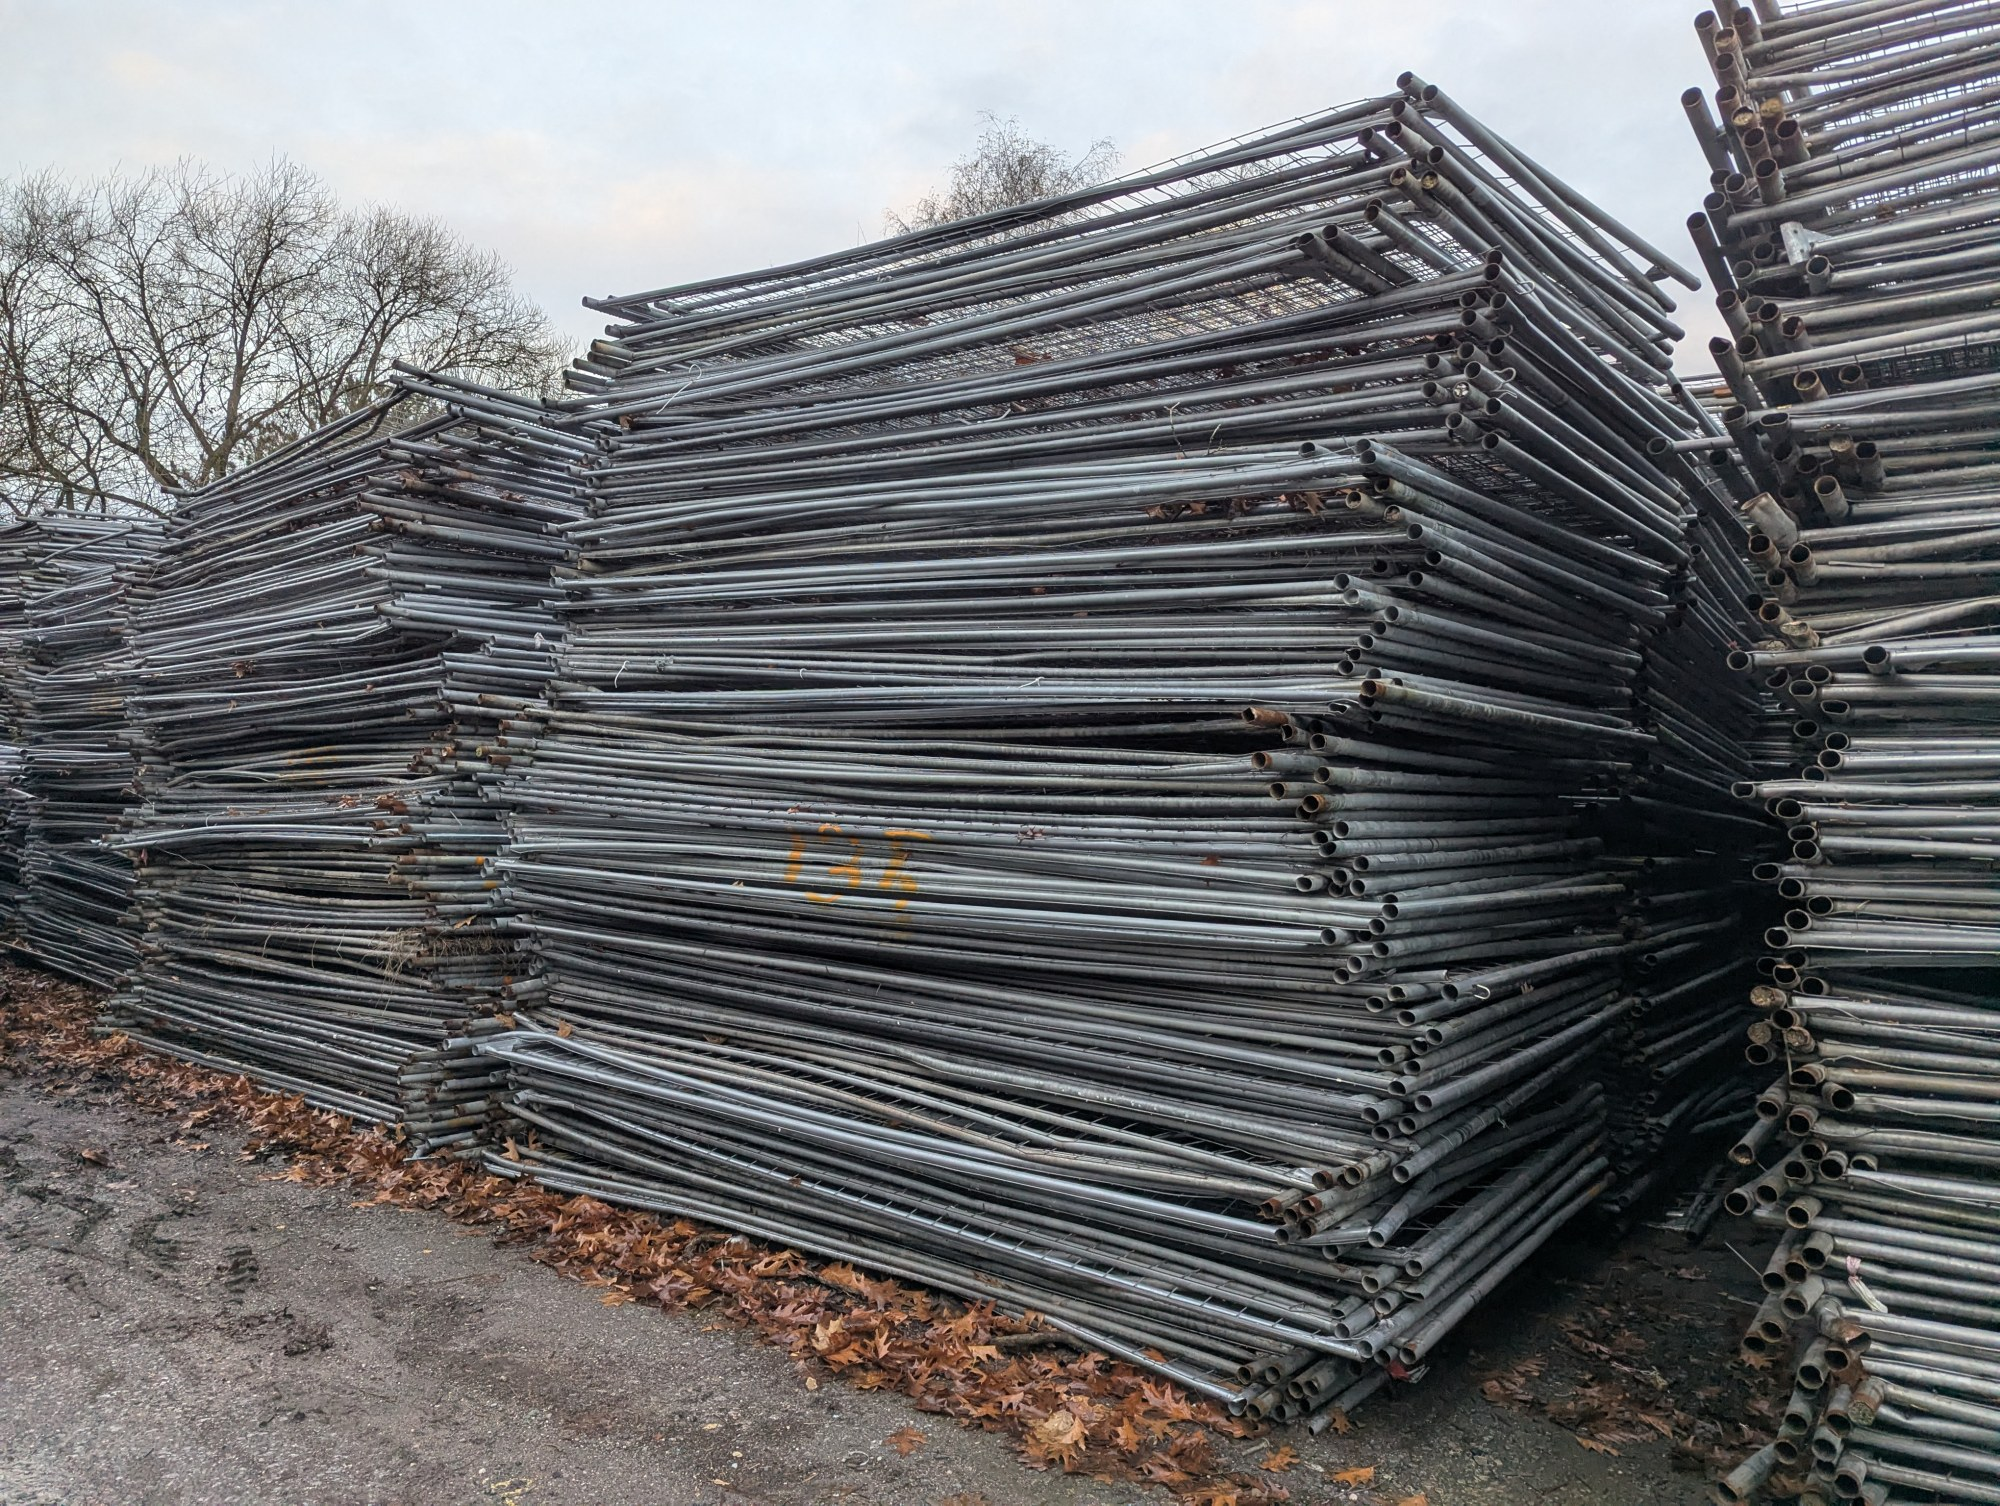
\includegraphics[width=0.52\textwidth]{abbildungen/real_stapel.jpg}
  \caption[Reale Stapelaufnahme]{Reale Aufnahme eines Stapels mobiler
  Bauzaunfelder. Zu detektieren ist die Stirnfläche der Rahmenrohre. Erkennbar
  sind die drei zentralen Schwierigkeiten: geringe Objektgröße, hohe
  Objektdichte und wechselseitige Verdeckung durch quer liegende Rohrschäfte.}
  \label{abb:realstapel}
\end{figure}

Aus Sicht der Bildverarbeitung ist das ein unangenehmer Spezialfall. Die Objekte
sind klein (gemessen 12--36\px{} Durchmesser im Original), dicht gepackt (im
Median rund ein Objektdurchmesser Abstand zum nächsten Nachbarn), untereinander
nahezu identisch und wechselseitig verdeckt. Erschwerend kommt hinzu, dass eine
Zählaufgabe jeden einzelnen Detektionsfehler unmittelbar in das Endergebnis
überträgt: Für eine exakte Zählung von 200 Objekten wäre eine Trefferquote von
über 99,5\,\% nötig.

Der eigentliche Engpass ist jedoch die Datenlage. COCO-vortrainierte Gewichte
enthalten keine Klasse \enquote{Bauzaunprofil}, und die Handannotation von
50--100 kleinen Boxen pro Bild über hunderte Bilder ist im Rahmen einer
Abschlussarbeit nicht leistbar. Zur Verfügung stehen neun aus Realbildern
ausgeschnittene Rohrprofile, sieben Hintergrundaufnahmen und zwei vollständig
annotierte Realbilder.

\section{Zielsetzung und Beitrag}

Der hier verfolgte Ansatz macht aus dieser Not das methodische Zentrum der
Arbeit: Trainiert wird \emph{ausschließlich} auf synthetischen Bildern, die aus
den neun Objektausschnitten und den sieben Hintergründen erzeugt werden;
Validierung und Test erfolgen auf den echten Aufnahmen. Damit ist die
Augmentierungspipeline nicht mehr eine Menge von Zusatztransformationen auf einem
vorhandenen Datensatz, sondern sie \emph{ist} der Datensatz: Sie definiert die
gesamte Trainingsverteilung.

Daraus ergibt sich die Gliederung der Arbeit, und es lohnt, die Rangfolge
ausdrücklich zu benennen. Ziel ist das \textbf{maschinelle Zählen} gestapelter
Bauzaunfelder. Der Schwerpunkt auf der Synthese-Pipeline ist diesem Ziel
\emph{nachgeordnet} und durch die Datenlage erzwungen: Ohne annotierte Realbilder
gibt es keinen Trainingsdatensatz, den man augmentieren könnte -- er muss erst
entstehen. Die untersuchten Architekturvarianten sind ein \emph{zweiter} Hebel
auf dieselbe Größe; sie stehen nicht in Konkurrenz zur Pipeline, sondern greifen
an derselben Ursache an, nämlich der geringen Objektgröße relativ zur
Gitterauflösung des Detektors. Entscheidungsmaß ist in beiden Fällen der
\textbf{Zählfehler} und nicht die mittlere Präzision -- eine Unterscheidung, die
sich in Abschnitt~\ref{sec:p2zaehlung} als folgenreich erweist.

Die Arbeit verfolgt drei Ziele. Erstens die \textbf{theoretische Einordnung der
Datenaugmentierung} (Kapitel~\ref{kap:augtheorie}): Was leistet Augmentierung
formal, welche Verfahrensklassen gibt es, welche Besonderheiten gelten bei der
Objektdetektion? Zweitens die \textbf{vollständige Dokumentation und Begründung
der konkreten Pipeline} (Kapitel~\ref{kap:pipeline} und
\ref{kap:trainingszeit}): Für jede Transformation werden Parameterbereich,
gemessener Ist-Anteil im erzeugten Datensatz und Begründung angegeben. Die
Begründung stützt sich dabei auf genau drei zulässige Quellen -- eine Messung an
den Realdaten, eine physikalische Randbedingung des Aufnahmegegenstands oder ein
in der Literatur belegtes Argument; wo keine dieser Quellen vorliegt, wird der
Wert ausdrücklich als Annahme gekennzeichnet. Drittens die
\textbf{experimentelle Bewertung} (Kapitel~\ref{kap:auswertung}) anhand von drei
Experimenten: Inferenzauflösung, Verdeckungsanteil in den Trainingsdaten und
Nutzen eines zusätzlichen hochauflösenden Detektionskopfes.

Der Beitrag liegt weniger in einer neuen Methode als in der Konsequenz, mit der
die Begründungspflicht durchgehalten wird. Copy-Paste-Synthese ist ein
etabliertes Verfahren \parencite{dwibedi2017,dvornik2018,ghiasi2021}; die Frage,
welche ihrer Bestandteile in einem konkreten industriellen Anwendungsfall tragen
und welche nicht, wird in der Literatur dagegen selten so kleinteilig
beantwortet.

\section{Aufbau}

Kapitel~\ref{kap:theorie} stellt die Grundlagen von Convolutional Neural Networks
und der YOLO26-Architektur bereit, Kapitel~\ref{kap:augtheorie} behandelt die
Datenaugmentierung allgemein und leitet sechs Anforderungen an die Pipeline ab.
Kapitel~\ref{kap:daten} vermisst das Quellmaterial -- diese Messungen sind die
Belegbasis aller Parameterentscheidungen. Kapitel~\ref{kap:pipeline} beschreibt
die Synthese-Pipeline, Kapitel~\ref{kap:trainingszeit} den Trainingsaufbau,
Kapitel~\ref{kap:auswertung} die Ergebnisse und Kapitel~\ref{kap:diskussion}
deren Tragfähigkeit und Grenzen; der Anhang nennt die Aufrufe der acht
Verarbeitungsstufen und enthält die vollständigen Parametertabellen.

\chapter{Theoretische Grundlagen}
\label{kap:theorie}

\section{Convolutional Neural Networks}
\label{sec:cnn}

\subsection{Grundprinzipien}
\label{sec:prinzipien}

Die drei genannten Prinzipien sind keine Implementierungsdetails, sondern
kodieren strukturelles Vorwissen über Bilddaten in die Netzarchitektur
(sogenannter \emph{induktiver Bias}). Sie werden im Folgenden formal hergeleitet.

Ein Grauwertbild wird als Funktion $x: \Omega \to \mathbb{R}$
auf dem diskreten Gitter $\Omega = \{0,\dots,H-1\} \times \{0,\dots,W-1\}$
aufgefasst; $x[i,j]$ bezeichnet den Wert an Position $(i,j)$. Eine Netzschicht
ist eine Abbildung, die eine Eingabe mit $C_{\text{in}}$ Kanälen auf eine
Ausgabe mit $C_{\text{out}}$ Kanälen überführt.

\absatz{Lokale rezeptive Felder.} In einer vollvernetzten Schicht berechnet sich
die Aktivierung eines Neurons $k$ aus \emph{allen} Eingangspixeln:
\begin{equation}
y_k = \sigma\!\left(\sum_{(i,j)\in\Omega} w_k[i,j]\,x[i,j] + b_k\right)
\label{eq:fc}
\end{equation}

Die Parameterzahl einer solchen Schicht beträgt
$C_{\text{out}} \cdot H \cdot W + C_{\text{out}}$. Für $H = W = 640$ und
lediglich $C_{\text{out}} = 100$ Neuronen ergeben sich bereits über 40~Millionen
Gewichte. Neben dem unmittelbaren Speicher- und Rechenaufwand ist dabei vor allem
die \textbf{Stichprobeneffizienz} problematisch: Ein vollvernetztes Netz besitzt
keinerlei architektonisches Vorwissen darüber, dass dasselbe visuelle Muster an
unterschiedlichen Bildpositionen dieselbe Bedeutung trägt, und müsste diese
Eigenschaft für jede Position separat aus Daten erlernen. Der entsprechende
Bedarf an Trainingsbeispielen ist in der Praxis kaum zu decken.

\begin{figure}[htbp]
\centering
\begin{tikzpicture}[scale=0.52, every node/.style={transform shape}]
  % ---- Panel a: vollvernetzt ----
  \begin{scope}[shift={(0,0)}]
    \foreach \i in {0,...,5}{\foreach \j in {0,...,5}{
      \fill[blue!12] (\i,\j) rectangle ++(1,1);
      \draw[gray!55,very thin] (\i,\j) rectangle ++(1,1);}}
    \node (outa) at (8.6,3) [circle,draw,fill=orange!25,minimum size=8mm] {$y_k$};
    \foreach \i in {0,...,5}{\foreach \j in {0,...,5}{
      \draw[gray!45,very thin] (\i+0.5,\j+0.5) -- (outa);}}
    \node[below] at (3,-0.35) {(a) vollvernetzt: $H\!\cdot\!W$ Gewichte je Neuron};
  \end{scope}
  % ---- Panel b: Faltung ----
  \begin{scope}[shift={(12.5,0)}]
    \foreach \i in {0,...,5}{\foreach \j in {0,...,5}{
      \draw[gray!55,very thin] (\i,\j) rectangle ++(1,1);}}
    \foreach \i in {2,3,4}{\foreach \j in {2,3,4}{
      \fill[blue!30] (\i,\j) rectangle ++(1,1);
      \draw[gray!70,very thin] (\i,\j) rectangle ++(1,1);}}
    \draw[very thick,orange!80!black] (2,2) rectangle (5,5);
    \node (outb) at (8.6,3) [circle,draw,fill=orange!25,minimum size=8mm] {$y[i,j]$};
    \foreach \i in {2,3,4}{\foreach \j in {2,3,4}{
      \draw[gray!60,very thin] (\i+0.5,\j+0.5) -- (outb);}}
    \node[below] at (3,-0.35) {(b) Faltung: $k^2$ Gewichte je Neuron};
  \end{scope}
\end{tikzpicture}
\caption[Vollvernetzte Schicht gegen Faltungsschicht]{Lokale rezeptive Felder.
(a)~In einer vollvernetzten Schicht nach Gleichung~\eqref{eq:fc} ist jedes
Ausgabeneuron mit allen $H\cdot W$ Eingangspixeln verbunden. (b)~In einer
Faltungsschicht nach Gleichung~\eqref{eq:conv} beschränkt sich die Summation auf
eine $k\times k$-Nachbarschaft; für $k=3$ sinkt die Zahl der Verbindungen je
Ausgabeneuron bei $640\times640$ Eingabe von 409\,600 auf 9. Zugleich wird
derselbe Kernel an allen Positionen verwendet (Weight Sharing), sodass die
Parameterzahl der Schicht unabhängig von der Bildgröße wird.}
\label{abb:rezeptivesfeld}
\end{figure}

Die klassische statistische Lerntheorie führt hohe Parameterzahlen darüber
hinaus auf eine erhöhte Modellkapazität und damit auf eine Neigung zur
Überanpassung zurück \parencite[Kap.~5]{goodfellow2016}. Für tiefe neuronale
Netze ist dieser Zusammenhang allerdings nicht ungebrochen gültig:
\textcite{zhang2017rethinking} zeigen experimentell, dass gängige Faltungsnetze
zufällige Beschriftungen der Trainingsdaten vollständig memorieren können und
dennoch auf realen Daten gut generalisieren. Dies ist ein Befund, der die klassische
Kapazitätsargumentation als alleinige Erklärung in Frage stellt. Der belastbare
Vorteil lokaler rezeptiver Felder liegt daher weniger in einer Vermeidung von
Überanpassung an sich als in der beschriebenen Stichprobeneffizienz und im
deutlich reduzierten Rechenaufwand.

In einer Faltungsschicht wird die Summation stattdessen auf eine lokale
Nachbarschaft $\mathcal{N}_{k \times k}$ der Größe $k \times k$ beschränkt:
\begin{equation}
y[i,j] = \sigma\!\left(\sum_{(u,v)\in\mathcal{N}_{k\times k}} w[u,v]\,
x[i+u,\,j+v] + b\right)
\label{eq:conv}
\end{equation}

Die Anzahl der Verbindungen je Ausgabeneuron sinkt damit von $H \cdot W$ auf
$k^2$ -- für $k = 3$ von 409\,600 auf 9 (Abbildung~\ref{abb:rezeptivesfeld}).
Die Rechtfertigung liegt in der lokalen Korrelationsstruktur natürlicher Bilder:
Die Korrelation benachbarter Pixelwerte fällt mit wachsendem Abstand rasch
ab, sodass weit entfernte Pixel für lokale Merkmalsentscheidungen kaum
Information beitragen \parencite{lecun1998}.

Das theoretische rezeptive Feld wächst mit der Netztiefe. Bezeichnet $r_\ell$
seine Kantenlänge nach Schicht $\ell$, $k_\ell$ die Kernelgröße und $s_\ell$ die
Schrittweite, der Laufindex $m$ im Produkt bezeichnet dieselbe Größe für die jeweil
 vorangehenden Schichten, so gilt die Rekursion
\begin{equation}
r_\ell = r_{\ell-1} + (k_\ell - 1)\prod_{m=1}^{\ell-1} s_m,
\qquad r_0 = 1.
\label{eq:rf}
\end{equation}

Bei reinen $3\times3$-Faltungen mit $s_m = 1$ wächst $r_\ell$ lediglich linear
($r_\ell = 2\ell + 1$); erst durch Schrittweiten $s_m = 2$ wächst das Produkt
exponentiell, sodass das rezeptive Feld schnell große Bildbereiche umfasst.
Hieraus entsteht die in Abschnitt~\ref{sec:hierarchie} beschriebene
Merkmalshierarchie. Zu beachten ist, dass das \emph{effektive} rezeptive Feld
kleiner ausfällt als dieses theoretische Maß:
\textcite{luo2016} zeigen, dass der Einfluss
$\partial y_{\text{Zentrum}} / \partial x[i,j]$ annähernd gaußförmig zum Zentrum
hin abfällt und nur ein Bruchteil des theoretischen Felds tatsächlich zur
Ausgabe beiträgt.

\absatz{Geteilte Gewichte (Weight Sharing).} Ohne Gewichtsteilung besäße jede
Position $(i,j)$ einen eigenen Kernel $w_{ij}$, was auf $H \cdot W \cdot k^2$
Parameter je Merkmalskarte führte. Weight Sharing bedeutet formal, dass
$w_{ij} = w$ für alle $(i,j)$ gilt; die Schicht wird dadurch zur diskreten
Faltung (genauer: Kreuzkorrelation)
\begin{equation}
y[i,j] = (w * x)[i,j] = \sum_{u,v} w[u,v]\,x[i+u,\,j+v],
\end{equation}
mit lediglich $k^2$ Parametern je Kernel. Für eine Schicht mit $C_{\text{in}}$
Eingangs- und $C_{\text{out}}$ Ausgangskanälen ergeben sich
$C_{\text{out}} \cdot C_{\text{in}} \cdot k^2 + C_{\text{out}}$ Parameter --
unabhängig von der Bildgröße. Dies ist der entscheidende Unterschied zur
vollvernetzten Schicht, deren Parameterzahl mit $H \cdot W$ skaliert.

Die zentrale Eigenschaft ist die \textbf{Translationsäquivarianz}. Bezeichnet
$(T_\tau x)[i,j] = x[i-\tau_1,\,j-\tau_2]$ die Verschiebung um $\tau$, so gilt
für die Faltungsoperation $f$:
\begin{equation}
f(T_\tau x) = T_\tau f(x).
\label{eq:aequivarianz}
\end{equation}

Eine Verschiebung der Eingabe führt also zu einer identischen Verschiebung der
Ausgabe-Merkmalskarte. Die Rechtfertigung ist die (näherungsweise) Stationarität
natürlicher Bildstatistik: Die relevanten lokalen Merkmale sind ortsunabhängig,
eine Kante bleibt eine Kante, unabhängig von ihrer Position. Zu betonen ist,
dass Äquivarianz nicht Invarianz bedeutet. Diese entsteht erst durch das
nachfolgend beschriebene Subsampling.

Aus der Gewichtsteilung folgen drei praktische Konsequenzen: erstens eine
erhöhte Dateneffizienz, da ein Muster, das nur an wenigen Positionen in den
Trainingsdaten vorkommt, dennoch überall erkannt wird; zweitens eine
Einschränkung des Hypothesenraums, da die Nebenbedingung $w_{ij} = w$ nur noch
translationsäquivariante Abbildungen zulässt -- eine Beschränkung, die dem
tatsächlichen Charakter der Aufgabe entspricht und in diesem Sinne als
struktureller Prior wirkt; drittens die Notwendigkeit mehrerer Kernel je
Schicht, da ein Kernel genau ein Muster repräsentiert
\parencite{lecun1998,goodfellow2016}.

\absatz{Räumliches Subsampling.} Für die Objekterkennung ist häufig
\emph{Invarianz} gegenüber kleinen Verschiebungen erwünscht, also
$f(T_\tau x) \approx f(x)$ für kleine $\|\tau\|$. Diese entsteht durch
stufenweise Reduktion der räumlichen Auflösung -- klassisch durch Pooling über
ein Fenster $\mathcal{P}$ der Größe $p \times p$ mit Schrittweite $s$:
\begin{equation}
y[i,j] = \max_{(u,v)\in\mathcal{P}} x[s\cdot i + u,\; s\cdot j + v]
\qquad \text{(Max-Pooling)}
\end{equation}

In modernen Architekturen wie YOLO26 wird dieselbe Auflösungsreduktion
überwiegend durch Faltungen mit Schrittweite $s = 2$ realisiert. In beiden Fällen
bleibt lediglich erhalten, \emph{ob} ein Merkmal innerhalb des Fensters auftrat,
nicht seine exakte Position. Für Verschiebungen $\|\tau\|_\infty < p$ innerhalb
desselben Pooling-Fensters bleibt die Ausgabe unverändert
\parencite{lecun1998,goodfellow2016}.

Die Ausgabegröße nach einer Schicht mit Kernelgröße $k$, Schrittweite $s$ und
Randauffüllung $p_{\text{pad}}$ beträgt
\begin{equation}
H_{\text{out}} = \left\lfloor
\frac{H_{\text{in}} + 2p_{\text{pad}} - k}{s} \right\rfloor + 1,
\end{equation}
woraus für $s = 2$ näherungsweise eine Halbierung je Stufe folgt. Nach $L$
solchen Stufen beträgt die Gesamtschrittweite $S = \prod_{\ell} s_\ell = 2^L$;
die Zahl der räumlichen Positionen sinkt dabei um den Faktor $S^2$, was den mit
der Tiefe wachsenden Kanalzahlen entgegenwirkt.

Der Preis ist ein Verlust an Ortsinformation, der bei kleinen Objekten kritisch
wird. Eine Zelle der Merkmalsebene mit Gesamtschrittweite $S$ entspricht einem
Bildbereich von $S \times S$ Pixeln. Ein Objekt mit Durchmesser $d$ Pixeln
belegt dort nur $d/S$ Zellen; für $d < S$ ist es kleiner als eine einzelne Zelle
und kann strukturell nicht mehr zuverlässig lokalisiert werden. Konkret gilt für
z.B. die feinste Detektionsebene P3 in YOLO26 mit $S = 8$: Ein Rohrprofil mit $d = 6$ Pixeln
unterschreitet diese Grenze. Dieser Zusammenhang begründet sowohl die
Multi-Skalen-Fusion moderner Detektoren (Abschnitt~\ref{sec:neck}) als auch die
in Abschnitt~\ref{sec:anwendung} diskutierten Gegenmaßnahmen der erhöhten
Eingabeauflösung bzw.\ Kachelung, die beide $d$ relativ zu $S$ vergrößern.

\absatz{Zusammenspiel.} Die drei Prinzipien reduzieren die Parameterzahl in
aufeinander aufbauenden Schritten: Lokale rezeptive Felder senken die
Verbindungen je Neuron von $H \cdot W$ auf $k^2$, Weight Sharing eliminiert die
Abhängigkeit der Parameterzahl von der Bildgröße, und Subsampling reduziert die
Zahl der zu verarbeitenden Positionen um $S^2$ und erzeugt zugleich lokale
Translationsinvarianz. Gemeinsam kodieren sie genau jene Annahmen, die für
Bilddaten zutreffen: Lokalität, Stationarität und Toleranz gegenüber kleinen
Verschiebungen. \textcite{lecun1998} formulierten diese Prinzipien am Beispiel
der Architektur LeNet-5 zur Ziffernerkennung.

\subsection{Aufbau eines CNNs}

Ein typisches CNN besteht aus einer Abfolge folgender Schichttypen:

\absatz{Faltungsschichten (Convolutional Layers).} Kernstück des CNNs ist die
diskrete Faltungsoperation. Ein Filterkern (Kernel), typischerweise der Größe
$3\times3$ oder $5\times5$, wird über das Eingabebild bzw.\ die Merkmalskarte
(Feature Map) geschoben. An jeder Position wird das Skalarprodukt zwischen
Kernelgewichten und dem darunterliegenden Bildausschnitt berechnet. Das Ergebnis
ist eine neue Merkmalskarte, die angibt, wie stark das vom Kernel
repräsentierte Muster an der jeweiligen Position ausgeprägt ist. Die Gewichte der
Kernel werden nicht manuell festgelegt, sondern im Training mittels
Backpropagation gelernt \parencite{lecun1998,goodfellow2016}.

\absatz{Aktivierungsfunktionen.} Auf jede Faltung folgt eine nichtlineare
Aktivierungsfunktion, ohne die das Netz nur lineare Abbildungen lernen könnte.
In modernen CNNs hat sich die Rectified Linear Unit (ReLU),
$f(x) = \max(0, x)$, sowie deren Varianten (z.\,B.\ SiLU/Swish) durchgesetzt, da
sie das Problem verschwindender Gradienten abmildert und effizient zu berechnen
ist \parencite{krizhevsky2012}.

\absatz{Pooling-Schichten.} Pooling-Operationen (meist Max-Pooling) reduzieren
die räumliche Auflösung der Merkmalskarten, indem sie z.\,B.\ aus jedem
$2\times2$-Bereich nur den Maximalwert übernehmen. Dies verringert den
Rechenaufwand, vergrößert das rezeptive Feld nachfolgender Schichten und sorgt
für eine gewisse Robustheit gegenüber kleinen Verschiebungen
\parencite{goodfellow2016}.

\absatz{Vollvernetzte Schichten (Fully Connected Layers).} Am Ende klassischer
CNN-Architekturen fassen vollvernetzte Schichten die extrahierten Merkmale
zusammen und bilden sie z.\,B.\ auf Klassenwahrscheinlichkeiten ab. In modernen
Detektionsarchitekturen werden sie zunehmend durch faltungsbasierte
Prädiktionsköpfe ersetzt.

\subsection{Merkmalshierarchie und Objektdetektion}
\label{sec:hierarchie}

Auf jede Faltung folgt eine nichtlineare Aktivierung -- heute überwiegend die
Rectified Linear Unit $f(x) = \max(0,x)$ oder Varianten wie SiLU
\parencite{krizhevsky2012} --, ohne die das Netz nur lineare Abbildungen lernen
könnte. Aus der Stapelung entsteht ein hierarchischer Aufbau der
Repräsentationen: Frühe Schichten reagieren auf Kanten und Farbverläufe, mittlere
auf Texturen und Teilstrukturen, tiefe auf semantische Objektbestandteile
\parencite{zeiler2014}. Diese datengetriebene Merkmalsextraktion tritt an die
Stelle des manuell entworfenen Feature Engineering und gilt als wesentlicher
Grund für die Leistungssprünge tiefer Netze \parencite{lecun2015}. Am Ende
klassischer Architekturen fassen vollvernetzte Schichten die Merkmale zusammen;
in modernen Detektoren sind sie vollständig durch Faltungen ersetzt
(Abschnitt~\ref{sec:neck}). Residualverbindungen \parencite{he2016} ermöglichen
das stabile Training sehr tiefer Netze und sind Standardbaustein nahezu aller
CNN-Backbones.

Für diese Arbeit ist nicht die Klassifikation relevant, sondern die
\textbf{Objektdetektion}: das gleichzeitige Lokalisieren und Klassifizieren
mehrerer Objekte. Zweistufige Detektoren erzeugen zunächst Regionsvorschläge und
klassifizieren diese anschließend \parencite{ren2015}; einstufige Detektoren
formulieren die Detektion als einmaliges Regressionsproblem und sagen in einem
Durchlauf direkt Boxen und Klassenwahrscheinlichkeiten vorher
\parencite{redmon2016,liu2016ssd}, was Echtzeitfähigkeit bei geringen
Genauigkeitseinbußen ermöglicht. Klassisch nachgeschaltet ist die
Non-Maximum Suppression (NMS), die redundante überlappende Detektionen anhand
ihrer Intersection over Union unterdrückt -- bei dicht gepackten gleichartigen
Objekten eine potenzielle Fehlerquelle.

\section{YOLO26}
\label{sec:yolo26}

\subsection{Einordnung und Neuerungen}

\enquote{You Only Look Once} wurde 2016 als erster echtzeitfähiger einstufiger
Detektor vorgestellt \parencite{redmon2016}; ab YOLOv8 übernahm Ultralytics die
Weiterentwicklung und etablierte ankerfreie, entkoppelte Detektionsköpfe
\parencite{sapkota2025}. YOLO26 wurde im September 2025 vorgestellt und
unterscheidet sich von YOLO11 durch vier koordinierte Änderungen: ein
Dual-Head-Design für NMS-freie Inferenz, den Wegfall der Distribution Focal Loss,
ProgLoss zusammen mit STAL sowie den MuSGD-Optimierer
\parencite{ultralytics2026,sapkota2025}.

Für diese Arbeit ist davon eine Änderung einschlägig: Die
\emph{Small-Target-Aware Label Assignment} garantiert positive Labelzuweisungen
auch für sehr kleine Objekte -- genau das Problem klassischer
Zuweisungsstrategien, das Abschnitt~\ref{sec:p2} quantifiziert.

\subsection{Backbone, Neck, Head und die Merkmalspyramide}
\label{sec:neck}

YOLO26 folgt der Dreiteilung \textbf{Backbone $\to$ Neck $\to$ Head}. Das
Backbone reduziert die räumliche Auflösung stufenweise per Stride-2-Faltungen
($1024 \to 512 \to 256 \to 128 \to 64 \to 32$ bei $1024$\px{} Eingabe), während
die Kanalzahl wächst -- räumliche Präzision wird gegen semantische Tiefe
getauscht. Jeder Faltung folgen Batch-Normalisierung und SiLU-Aktivierung; die
Blöcke sind im CSP-Stil mit Residualverbindungen organisiert, am Ende aggregiert
ein SPPF-Modul Kontext über mehrere Pooling-Größen.

\absatz{Neck.} Das Neck verbindet die Auflösungsstufen in beide Richtungen
(FPN/PAN-Prinzip, \cite{lin2017fpn}): Tiefe, semantisch reiche Merkmalskarten
werden hochskaliert und mit den feinen, ortsgenauen Karten früherer Stufen
zusammengeführt, und umgekehrt. Der Head erhält dadurch mehrere Ausgabeebenen,
die nach Objektgröße zuständig sind. Die Standardkonfiguration liefert drei
Ebenen P3/P4/P5 mit den Gesamtschrittweiten 8/16/32; zusätzlich existiert eine
Konfiguration mit einer vierten, feineren Ebene \textbf{P2 mit Schrittweite~4}
(Abbildung~\ref{abb:pyramide}). Sie ist der Gegenstand von
Abschnitt~\ref{sec:p2}.

\begin{figure}[htbp]
\centering
\begin{tikzpicture}[x=1cm,y=1cm]
  % ---- Merkmalsebenen als Quadrate, Seitenlaenge proportional zur Gittergroesse
  \draw[fill=red!8,dashed,thick,red!60!black] (0,0) rectangle (4,4);
  \draw[step=0.5,gray!35,very thin] (0,0) grid (4,4);
  \draw[fill=blue!8] (4.7,0) rectangle (6.7,2);
  \draw[step=0.5,gray!35,very thin] (4.7,0) grid (6.7,2);
  \draw[fill=blue!8] (7.4,0) rectangle (8.4,1);
  \draw[step=0.5,gray!35,very thin] (7.4,0) grid (8.4,1);
  \draw[fill=blue!8] (9.1,0) rectangle (9.6,0.5);

  \node[below,align=center,font=\scriptsize] at (2,-0.2)
       {\textbf{P2} $\;$ Stride 4\\$256\times256$\\65\,536 Positionen};
  \node[below,align=center,font=\scriptsize] at (5.7,-0.2)
       {\textbf{P3} $\;$ Stride 8\\$128\times128$\\16\,384};
  \node[below,align=center,font=\scriptsize] at (7.9,-0.2)
       {\textbf{P4} $\;$ 16\\$64^2$\\4\,096};
  \node[below,align=center,font=\scriptsize] at (9.35,-0.2)
       {\textbf{P5} $\;$ 32\\$32^2$\\1\,024};

  \node[above,font=\scriptsize,red!60!black,align=center] at (2,4.15)
       {\emph{nur in der Variante} \code{-p2}};
  \node[above,font=\scriptsize,align=center] at (7.0,4.15)
       {Standardkonfiguration P3--P5};
  \draw[decorate,decoration={brace,amplitude=4pt},gray!60!black]
       (4.7,4.05) -- (9.6,4.05);
  \node[font=\scriptsize,align=left,anchor=west] at (10.1,2.6)
       {kleine\\Objekte};
  \node[font=\scriptsize,align=left,anchor=west] at (10.1,1.2)
       {große\\Objekte};
  \draw[-{Latex[length=1.6mm]},gray!60!black] (10.35,2.3) -- (10.35,1.6);
\end{tikzpicture}
\caption[Merkmalsebenen des Detektionskopfes]{Merkmalsebenen des
Detektionskopfes bei einer Eingabe von $1024\times1024$ Pixeln. Die
Seitenlänge der Quadrate ist proportional zur Gittergröße. Jede Zelle einer
Ebene mit Schrittweite $S$ entspricht einem Bildbereich von $S \times S$ Pixeln
und sagt Boxkoordinaten sowie Klassen-Scores vorher. Die Standardkonfiguration
nutzt P3--P5; die Variante \code{-p2} ergänzt die Ebene P2 mit Schrittweite~4,
die allein mehr Prädiktionspositionen enthält als P3, P4 und P5 zusammen.}
\label{abb:pyramide}
\end{figure}

\absatz{Head.} Das ursprüngliche YOLOv1 endete in zwei vollvernetzten Schichten
\parencite{redmon2016}, die den überwiegenden Teil aller Parameter enthielten,
die Eingabegröße fixierten und die räumliche Struktur zerstörten. Moderne
YOLO-Architekturen sind dagegen vollständig faltungsbasiert: Der Kopf besteht aus
kleinen Faltungsstapeln, die in $1\times1$-Faltungen münden. Eine
$1\times1$-Faltung ist mathematisch äquivalent zu einer vollvernetzten Schicht
über die Kanaldimension, wird aber \textbf{positionsgeteilt} angewendet --
dieselbe Operation verarbeitet die Kanäle jeder Gitterzelle separat. Das erhält
die Translationsäquivarianz bis in die Ausgabeschicht und macht das Netz
unabhängig von einer festen Eingabegröße. Der Kopf ist zusätzlich
\emph{entkoppelt} (getrennte Zweige für Klassifikation und Boxregression) und
\emph{ankerfrei}: Jede Gitterzelle regressiert direkt die Abstände zu den vier
Boxrändern. Damit ist die Zahl der Gitterzellen -- und nicht die Zahl der
Ankerboxen -- die Größe, die bestimmt, wie fein Objekte überhaupt aufgelöst
werden können.

\section{Anwendung auf die Zählung gestapelter Bauzäune}
\label{sec:anwendung}

Ein YOLO-Modell wird per Transfer Learning von COCO-vortrainierten Gewichten
\parencite{yosinski2014} auf eine einzige Objektklasse feinabgestimmt; die
Zaunanzahl ergibt sich aus der Zahl der detektierten Stirnflächen. Die
hierarchische Merkmalsextraktion des Backbones ist dafür gut geeignet:
Kreisförmige Metallprofile mit charakteristischem Hell-Dunkel-Verlauf sind
visuell einfache, texturarme Objekte, die bereits mittlere Netzschichten
repräsentieren können. YOLO26 adressiert die kritischen Eigenschaften des
Problems konzeptionell direkt: STAL und ProgLoss verbessern die Erkennung kleiner
Objekte, und die NMS-freie Inferenz eliminiert einen bei dicht gepackten
gleichartigen Objekten systematisch fehleranfälligen Hyperparameter -- ein zu
niedriger IoU-Schwellwert unterdrückt korrekte Detektionen benachbarter Rohre
(Unterzählung), ein zu hoher lässt Duplikate zu (Überzählung). Da es sich um ein
Ein-Klassen-Problem mit geometrisch einfachen Objekten handelt, genügen kleine
Modellvarianten. Anders als dichtebasierte Zählverfahren
\parencite{lempitsky2010,zhang2016counting} liefert die detektionsbasierte
Zählung pro Objekt eine sichtbare Box; Fehlzählungen sind damit lokalisierbar und
im Einsatz korrigierbar.

Drei Grenzen sind kritisch. Erstens die \textbf{Auflösung}: Die
Standard-Eingabegröße von $640\times640$ ist für diese Aufgabe zu klein -- wird
eine hochaufgelöste Stapelaufnahme darauf herunterskaliert, schrumpfen die
Profile auf wenige Pixel und unterschreiten die Auflösungsgrenze der P3-Ebene.
Abhilfe schaffen eine erhöhte Eingabeauflösung (Rechenaufwand wächst
quadratisch), eine Kachelung des Bildes \parencite{akyon2022sahi} oder ein
feinerer Detektionskopf (Abschnitt~\ref{sec:p2}). Zweitens die
\textbf{Verdeckung}: Verkippte Zäune verdecken benachbarte Profile, und visuell
ähnliche Strukturen -- Gitterknoten, Löcher im Maschendraht, Schattenspalten --
drohen als Falschpositive. Drittens der \textbf{Datenbedarf}: Ein eigener
annotierter Datensatz ist unumgänglich und muss die reale Varianz abdecken. Genau
hier setzt der Praxisteil an -- die Domänenlücke wird nicht durch Handannotation
geschlossen, sondern durch eine Synthese-Pipeline, deren Entwurf Gegenstand der
Kapitel~\ref{kap:augtheorie} bis \ref{kap:trainingszeit} ist.

\chapter{Datenaugmentierung}
\label{kap:augtheorie}

\section{Begriff, Formalisierung und Wirkmechanismen}
\label{sec:augformal}

Datenaugmentierung bezeichnet die künstliche Vergrößerung eines
Trainingsdatensatzes durch Transformationen, die den semantischen Gehalt der
Beispiele -- und damit ihre Beschriftung -- erhalten \parencite{shorten2019}. Sei
$D = \{(x_i, y_i)\}_{i=1}^{n}$ der Datensatz, $\mathcal{T}$ eine Familie von
Transformationen mit einer Verteilung $p(t)$ und $\tau_t$ die zu $t$ gehörende
\emph{Labeltransformation}. Anstelle des empirischen Risikos minimiert das
Training dann das \emph{augmentierte} Risiko
\begin{equation}
\hat{R}_{\text{aug}}(f) \;=\; \frac{1}{n}\sum_{i=1}^{n}
\mathbb{E}_{t \sim p(t)}\Big[ L\big(f(t(x_i)),\, \tau_t(y_i)\big) \Big],
\label{eq:erm-aug}
\end{equation}
also das Risiko gemittelt über eine \emph{Umgebung} jedes Datenpunkts --
die Vicinal Risk Minimization von \textcite{chapelle2001}.

\absatz{Die Gleichung im Einzelnen.} Weil auf ihr die gesamte Argumentation der
folgenden Kapitel aufbaut, seien die vier Bestandteile benannt, die bei der
Detektion nicht selbsterklärend sind:

\begin{description}[leftmargin=4.2em,style=sameline,itemsep=0pt,
                    font=\normalfont]
  \item[$(x_i, y_i)$] das $i$-te Trainingsbeispiel. Bei der Detektion ist $y_i$
  keine einzelne Zahl, sondern eine \emph{Menge} von Boxen mit Klassenangabe.
  \item[$\mathcal{T}$] die Familie der überhaupt zugelassenen Transformationen --
  die Antwort auf die Frage, \emph{welche} Operationen erlaubt sind.
  \item[$p(t)$] die Verteilung über $\mathcal{T}$ -- die Antwort auf
  \emph{wie häufig} und \emph{wie stark}. Sie ist das, was die
  Parametertabellen dieser Arbeit dokumentieren.
  \item[$\tau_t$] die zu $t$ gehörende Labeltransformation: wie $y$ verändert
  werden muss, damit es $t(x)$ noch korrekt beschreibt.
\end{description}

Der Unterschied zum gewöhnlichen empirischen Risiko
\[
\hat{R}(f) \;=\; \frac{1}{n}\sum_{i=1}^{n} L\big(f(x_i),\, y_i\big)
\]
liegt allein im Erwartungswert: Statt jedes Beispiel genau in der Form zu sehen,
in der es aufgenommen wurde, sieht das Netz eine ganze Umgebung davon. Weil
$\mathcal{T}$ überabzählbar ist, wird der Erwartungswert praktisch durch eine
Monte-Carlo-Näherung mit \emph{einer} Ziehung je Bild und Epoche ersetzt. Daraus
folgt eine Konsequenz, die in Abschnitt~\ref{sec:ablation} messbar wird: Starke
Augmentierung und kurzes Training passen nicht zusammen -- der Arm ohne
Verdeckung sättigte dort bereits in Epoche~3, die beiden augmentierten
verbesserten sich bis zur letzten Epoche.

\absatz{Was in dieser Arbeit \emph{ein} $t$ ist.} Keine einzelne Operation,
sondern ein Parametervektor über alle Stufen der Pipeline -- etwa
\enquote{Hintergrund 3, Zoom 1,42, horizontal gespiegelt, Objektrotation
$137^\circ$, Achsverhältnis 0,81, Helligkeit $\times 0{,}92$, Gamma 1,08,
Rauschangleich $\sigma = 4{,}1$, Schlagschatten, JPEG-Qualität 71}. Die
Verteilung $p(t)$ faktorisiert dabei über die einzelnen Transformationen: Die
Anteile der Parametertabelle sind unabhängige Ziehungen. Zwei Ausnahmen sind
bewusst gesetzt und folgen aus Anforderung~A3 -- Objektgröße und
Hintergrundzoom sind gekoppelt (Gleichung~\eqref{eq:zoom}), und die Größen aller
Instanzen eines Clusters hängen an einer gemeinsamen Basisgröße. Eine
unabhängige Ziehung wäre dort physikalisch unmöglich.


Für den vorliegenden Fall lohnt eine letzte Lesart. Weil die Trainingsdaten
nicht erweitert, sondern \emph{erzeugt} werden, ist $n$ winzig -- als
Ausgangsmenge lassen sich die neun Objektausschnitte und sieben Hintergründe
lesen, und $t$ ist der gesamte Generatordurchlauf. Die 6000 Trainingsbilder sind
dann 6000 Ziehungen aus $p(t)$. Die gesamte Vielfalt des Datensatzes steckt
damit in $p(t)$ und in keinem einzigen aufgenommenen Bild -- weshalb die
Dokumentation von $p(t)$ in dieser Arbeit die Dokumentation des Datensatzes
\emph{ist}.

\absatz{Die Labeltransformation ist der kritische Teil.} Neben $t$ tritt in
Gleichung~\eqref{eq:erm-aug} stets $\tau_t$ auf. Bei der Klassifikation ist
$\tau_t = \mathrm{id}$ -- eine gespiegelte Katze bleibt eine Katze --, weshalb
Augmentierung dort begrifflich mit \enquote{label-erhaltend} gleichgesetzt wird.
Bei der Objektdetektion ist $\tau_t \neq \mathrm{id}$: Boxkoordinaten müssen
mittransformiert werden. Ist $\tau_t$ nur \emph{näherungsweise} bekannt, so
entsteht Rauschen im Zielsignal -- genau die in
Abschnitt~\ref{sec:augdetektion} behandelte Fehlerquelle, und der Grund für die
Arbeitsteilung zwischen Generator und Trainingszeit in
Kapitel~\ref{kap:pipeline}.

Die Literatur unterscheidet drei Wirkmechanismen. \emph{(1) Kodierung von
Invarianzen:} Bildet $\mathcal{T}$ eine Gruppe, unter deren Wirkung die
Beschriftung invariant ist, so entspricht die Mittelung in
Gleichung~\eqref{eq:erm-aug} einer Projektion auf den Raum der invarianten
Funktionen, und \textcite{chen2020group} zeigen, dass diese Orbit-Mittelung die
Varianz des Schätzers reduziert, ohne den Bias zu erhöhen -- Augmentierung ist
also strikt vorteilhaft, sofern die angenommene Invarianz gilt.
\emph{(2) Regularisierung durch Rauschen:} Für photometrische Störungen, Rauschen
und Unschärfe -- Perturbationen ohne Gruppenstruktur -- zeigt
\textcite{bishop1995}, dass Training mit Rauschen äquivalent zu einer
Tikhonov-Regularisierung ist und die gelernte Funktion messbar glättet
\parencite[vgl.\ auch][]{dao2019}. \emph{(3) Erweiterung des Trägers:}
Augmentierung erzeugt Konfigurationen, die im Originaldatensatz nicht vorkommen --
bei nur neun Quellobjekten der dominierende Effekt. Die Grenze ist gleichzeitig
offensichtlich: Augmentierung erzeugt keine neue \emph{Information} über die
Objektklasse, sondern verteilt die vorhandene über einen größeren Bereich des
Eingaberaums.

\absatz{Verhältnis zum induktiven Bias.} Die Faltungsarchitektur garantiert
Translationsäquivarianz \emph{strukturell}
(Gleichung~\eqref{eq:aequivarianz}). Für alle anderen erwünschten Invarianzen --
Rotation, Skalierung, Beleuchtung, Farbstich, Teilverdeckung -- gibt es keine
solche Garantie; Augmentierung bringt sie auf der \emph{Datenseite} ein. Daraus
folgt der wesentliche Entwurfsgrundsatz: Antrainiert werden dürfen nur
Invarianzen, die in der Domäne \emph{tatsächlich gelten}. Eine Augmentierung, die
eine nicht vorhandene Invarianz erzwingt, verschlechtert das Modell, weil sie
diskriminative Information entfernt. Volle Rotationsinvarianz ist bei einem
Rohrende korrekt, weil Kamerarollwinkel und Stapelausrichtung beliebig sind; bei
einem Verkehrszeichen wäre sie falsch.

\section{Verfahrensüberblick}
\label{sec:augtaxonomie}

Tabelle~\ref{tab:taxonomie} im Anhang ordnet die etablierten Verfahrensklassen
und nennt jeweils, ob und wie sie hier eingesetzt werden. Zwei Entscheidungen
folgen daraus. Erstens sind fertige Bibliotheken wie Albumentations
\parencite{buslaev2020} nicht verwendet, weil die zentrale Anforderung -- eine
exakte Sichtbarkeitsbuchhaltung über die Malreihenfolge mehrerer eingefügter
Objekte (Abschnitt~\ref{sec:sichtbarkeit}) -- außerhalb ihres Funktionsumfangs
liegt. Zweitens sind Verfahren, die $p(t)$ selbst optimieren (AutoAugment
\parencite{cubuk2019}, RandAugment \parencite{cubuk2020}, Detektions-Policies
\parencite{zoph2020}), nicht anwendbar: Jede Suche setzt einen Bewertungssplit
voraus, und hier existiert genau \emph{ein} reales Validierungsbild.

Eine Untergruppe rechtfertigt eine eigene Pipelinestufe. Cutout, Random Erasing
und Hide-and-Seek löschen zufällige Bildbereiche, damit ein Netz die Evidenz über
das gesamte Objekt verteilt statt an einem einzigen diskriminativen Teilmerkmal
zu hängen; \textcite{wang2017afastrcnn} erzeugen solche Verdeckungen sogar
adversarial. Hier ist Verdeckung allerdings nicht bloß eine Regularisierungsidee,
sondern der Normalfall der Zieldomäne -- weshalb sie durch physikalisch plausible
Okkluder erzeugt wird und nicht durch gelöschte Rechtecke.

\section{Besonderheiten bei der Objektdetektion}
\label{sec:augdetektion}

Die Besonderheit der Objektdetektion liegt in der Box: Sie ist ein achsparalleles
Rechteck und damit ein grobes Modell des Objektumrisses -- bei 20\px{} großen,
runden Objekten ein fragiles. Zwei Folgen betreffen die beiden Seiten der
Pipeline. Am \emph{Eingang} ist zu klären, welche Transformation angewandt werden
darf, ohne das Regressionsziel zu verfälschen
(Abschnitt~\ref{sec:boxrotation}); am \emph{Ausgang}, welche Metrik gelesen
werden darf, ohne einen Konventionsunterschied für einen Modellfehler zu halten.
Beide laufen auf dieselbe Größe hinaus: das Verhältnis eines absoluten
Boxfehlers zur Objektgröße. Hinzu kommt eine dritte Folge, die nicht die Box
betrifft, sondern das Gitter -- Objekte unterhalb der Zellbreite erhalten unter
Umständen gar keine Labelzuweisung (Abschnitt~\ref{sec:ioukleinobjekt}).

\subsection{Achsparallele Boxen und Rotation}
\label{sec:boxrotation}

Bounding Boxes sind achsparallel. Wird ein Bild um $\theta$ gedreht, ist die
transformierte Box das nicht mehr; die Implementierung nimmt daher die
umschließende Hülle, deren Kanten auf $w\,|\cos\theta| + h\,|\sin\theta|$
bzw.\ $w\,|\sin\theta| + h\,|\cos\theta|$ wachsen.

Entscheidend ist der Fall eines rotationssymmetrischen Objekts -- und genau das
ist eine Rohrstirnfläche: Die \emph{korrekte} Box eines Kreises ändert sich unter
Rotation nicht, die \emph{transformierte} wächst dennoch um
$|\cos\theta| + |\sin\theta|$. Die Überlappung zwischen beiden beträgt
\begin{equation}
\mathrm{IoU}(\theta) \;=\; \frac{1}{(|\cos\theta| + |\sin\theta|)^2}
\;=\; \frac{1}{1 + |\sin 2\theta|}.
\label{eq:ioutheta}
\end{equation}
Die rechte Form macht den Verlauf unmittelbar lesbar: Die Überlappung fällt
monoton mit $|\sin 2\theta|$ und erreicht bei $\theta = 45^\circ$ ihr Minimum
$\tfrac12$. Die Schwelle 0,75 wird bereits bei $\sin 2\theta = \tfrac13$, also
bei $\theta = 9{,}7^\circ$, unterschritten.

\begin{figure}[htbp]
\centering
\begin{tikzpicture}
\begin{scope}
  \fill[blue!14] (0,0) circle (1.1);
  \draw[blue!60!black,semithick] (0,0) circle (1.1);
  \begin{scope}[rotate=10]
    \draw[gray!85,semithick] (-1.1,-1.1) rectangle (1.1,1.1);
  \end{scope}
  \draw[dashed,thick] (-1.1,-1.1) rectangle (1.1,1.1);
  \draw[very thick,orange!85!black] (-1.2744,-1.2744) rectangle (1.2744,1.2744);
  \draw[->,>=stealth,gray!70] (1.15,0) arc (0:10:1.15);
  \node[font=\scriptsize] at (1.50,0.12) {$\theta$};
  \draw[|<->|,gray!60!black,thin] (-1.1,-1.52) -- (1.1,-1.52);
  \node[font=\scriptsize,anchor=north] at (0,-1.50) {$a$};
  \draw[|<->|,orange!85!black,thin] (-1.2744,-2.05) -- (1.2744,-2.05);
  \node[font=\scriptsize,anchor=north,orange!85!black] at (0,-2.03)
       {$a\,(|\cos\theta| + |\sin\theta|)$};
  \node[font=\scriptsize,anchor=north] at (0,-2.55) {(a)};
\end{scope}
\begin{scope}[shift={(5.0,-1.75)}]
  \draw[->,semithick] (0,0) -- (5.1,0) node[below right,font=\scriptsize] {$\theta$};
  \draw[->,semithick] (0,0) -- (0,3.4) node[left,font=\scriptsize] {$\mathrm{IoU}$};
  \foreach \t in {0,10,20,30,40}
    \draw[semithick] ({\t*0.1},0) -- ({\t*0.1},-0.08)
          node[below,font=\scriptsize] {$\t^\circ$};
  \foreach \v/\l in {0/{0,5}, 0.6/{0,6}, 1.2/{0,7}, 1.8/{0,8}, 2.4/{0,9}, 3.0/{1,0}}
    \draw[semithick] (0,\v) -- (-0.08,\v) node[left,font=\scriptsize] {\l};
  \draw[dashed,red!70!black] (0,1.5) -- (5.0,1.5);
  \node[font=\scriptsize,red!70!black,anchor=south east] at (5.02,1.55)
        {Schwelle \mAPseven};
  \draw[dashed,gray!60] ({9.74*0.1},0) -- ({9.74*0.1},1.5);
  \fill[red!70!black] ({9.74*0.1},1.5) circle (1.6pt);
  \node[font=\scriptsize,anchor=west] at (1.12,0.80) {$\theta = 9{,}7^\circ$};
  \draw[very thick,orange!85!black,smooth]
    plot[domain=0:45,samples=91]
    ({\x*0.1}, {(1/(1+sin(2*\x)) - 0.5)*6});
  \node[font=\scriptsize,anchor=north] at (2.5,-0.55) {(b)};
\end{scope}
\end{tikzpicture}
\caption[Boxaufblähung unter Bildrotation]{Bildrotation als Quelle von
Labelrauschen. (a)~Ein rotationssymmetrisches Objekt behält unter Rotation
dieselbe korrekte Box (schwarz gestrichelt); die mitgedrehte Box (grau) und ihre
achsparallele Hülle (orange) sind jedoch größer. (b)~Verlauf nach
Gleichung~\eqref{eq:ioutheta}: Bei $2^\circ$ liegt die Überlappung noch bei
0,935, bei $10^\circ$ bereits bei 0,745 und bei $45^\circ$ bei 0,500.}
\label{abb:boxrotation}
\end{figure}

Für ein Objekt von 25\px{} Durchmesser wächst die Boxkantenlänge bei $10^\circ$
um rund 4\px{} -- systematisches Rauschen im Zielsignal der Boxregression
(Abbildung~\ref{abb:boxrotation}). Die Konsequenz: Bildrotation, Scherung und Perspektive dürfen \emph{nicht} als
bildweite Trainingszeit-Augmentierung eingesetzt werden, wenn dieselbe Variation
auch label-exakt erzeugt werden kann -- was ein Generator leistet, der die Box
nach der Transformation aus der transformierten Alphamaske neu bestimmt.

\subsection{Kleine Objekte, Auflösung und Labelzuweisung}
\label{sec:ioukleinobjekt}

Verschiebt man eine quadratische Box der Kantenlänge $d$ um $\delta$ Pixel in
einer Achse, so gilt
\begin{equation}
\mathrm{IoU} \;=\; \frac{(d-\delta)\,d}{2d^2 - (d-\delta)\,d}
\;=\; \frac{1 - \delta/d}{1 + \delta/d} .
\label{eq:ioushift}
\end{equation}
Der Fehler wirkt ausschließlich über das \emph{Verhältnis} $\delta/d$: Für ein
20\px-Objekt kostet ein Boxfehler von 2\px{} bereits 0,18 IoU, bei diagonaler
Verschiebung 0,32; für ein 200\px-Objekt wäre derselbe absolute Fehler mit 0,02
IoU unsichtbar. \mAPall{} ist bei dieser Objektgröße folglich mehr ein Maß für
die Pixelauflösung als für die Detektionsqualität.

\begin{figure}[htbp]
\centering
\begin{tikzpicture}
\begin{scope}
  \node[font=\scriptsize,anchor=west] at (-0.15,3.35)
       {\textcolor{black}{$-\,-$ Ground Truth}\quad
        \textcolor{orange!85!black}{$-\!-$ Vorhersage}};
  \fill[pattern=north east lines,pattern color=orange!45]
       (0.72,0) rectangle (2.4,2.4);
  \draw[dashed,thick] (0,0) rectangle (2.4,2.4);
  \draw[very thick,orange!85!black] (0.72,0) rectangle (3.12,2.4);
  \draw[|<->|,gray!60!black,thin] (0,2.66) -- (0.72,2.66)
        node[midway,above,font=\scriptsize,inner sep=1pt] {$\delta$};
  \draw[|<->|,gray!60!black,thin] (-0.28,0) -- (-0.28,2.4)
        node[midway,fill=white,inner sep=1pt,font=\scriptsize] {$d$};
  \node[font=\scriptsize,anchor=north] at (1.5,-0.25) {(a)};
\end{scope}
\begin{scope}[shift={(5.0,-0.35)}]
  \draw[->,semithick] (0,0) -- (4.7,0)
        node[below right,font=\scriptsize] {$\delta/d$};
  \draw[->,semithick] (0,0) -- (0,3.4) node[left,font=\scriptsize] {$\mathrm{IoU}$};
  \foreach \t/\l in {0.1/{0,1}, 0.2/{0,2}, 0.3/{0,3}, 0.4/{0,4}}
    \draw[semithick] ({\t*8},0) -- ({\t*8},-0.08)
          node[below,font=\scriptsize] {\l};
  \foreach \v/\l in {0.75/{0,25}, 1.5/{0,5}, 2.25/{0,75}, 3.0/{1,0}}
    \draw[semithick] (0,\v) -- (-0.08,\v) node[left,font=\scriptsize] {\l};
  \draw[dashed,red!70!black] (0,1.5) -- (4.6,1.5);
  \draw[dashed,red!30!black] (0,2.25) -- (4.6,2.25);
  \node[font=\scriptsize,red!30!black,anchor=north east,fill=white,
        inner sep=1pt] at (4.58,2.21) {Schwelle 0,75};
  \node[font=\scriptsize,red!70!black,anchor=south east,fill=white,
        inner sep=1pt] at (4.58,1.53) {Schwelle 0,50};
  \draw[very thick,orange!85!black,smooth]
    plot[domain=0:0.45,samples=60] ({\x*8}, {((1-\x)/(1+\x))*3});
  \draw[very thick,blue!60!black,densely dashed,smooth]
    plot[domain=0:0.45,samples=60]
    ({\x*8}, {(((1-\x)*(1-\x))/(2-(1-\x)*(1-\x)))*3});
  \node[font=\scriptsize,anchor=west,orange!85!black] at (3.68,1.14)
       {achsparallel};
  \node[font=\scriptsize,anchor=west,blue!60!black] at (3.68,0.53)
       {diagonal};
  \fill[orange!85!black] (0.8,{(0.9/1.1)*3}) circle (1.5pt);
  \fill[blue!60!black]   (0.8,{(0.81/1.19)*3}) circle (1.5pt);
  \node[font=\scriptsize,anchor=south west,fill=white,inner sep=1pt]
       at (0.90,{(0.9/1.1)*3}) {$\delta=2$\,px bei $d=20$\,px};
  \node[font=\scriptsize,anchor=north] at (2.3,-0.55) {(b)};
\end{scope}
\end{tikzpicture}
\caption[Empfindlichkeit der IoU gegenüber Boxversatz]{Empfindlichkeit der IoU
gegenüber einem Boxversatz. (a)~Zwei Boxen der Kantenlänge $d$, um $\delta$
verschoben; schraffiert der Schnitt. (b)~Verlauf nach
Gleichung~\eqref{eq:ioushift} für achsparallele und für diagonale Verschiebung.
Der Fehler wirkt allein über das Verhältnis $\delta/d$: Die Schwelle 0,75 wird
bei $\delta/d = 1/7$ unterschritten (2,9\px{} bei einem 20\px-Objekt), die
Schwelle 0,50 bei $\delta/d = 1/3$ (6,7\px).}
\label{abb:iouversatz}
\end{figure}

Detektoren verarbeiten Bilder in einer festen Netzeingangsgröße $M$
(\code{imgsz}); ein Bild mit längster Kante $N$ wird um $M/N$ skaliert. Ein
Objekt mit Durchmesser $d$ erreicht das Netz damit mit
\begin{equation}
d_{\text{eff}} \;=\; d \cdot \frac{M}{N} .
\label{eq:deff}
\end{equation}
Für $N = 2459$, $d = 27$\px{} und $M = 640$ ergibt das
$d_{\text{eff}} = 7{,}0$\px{} -- weniger als die Schrittweite $S = 8$ der
feinsten Standard-Detektionsebene. Wie folgenreich das ist, zeigt die Zahl der
Gitterzellen, deren Zentrum in das Objekt fällt und die damit bei einem
ankerfreien Kopf überhaupt als positive Zuweisung in Frage kommen. Für ein
kreisförmiges Objekt vom Durchmesser $d$ auf einer Ebene mit Schrittweite $S$
beträgt dieser Erwartungswert, gemittelt über die Lage des Objektzentrums im
Gitter,
\begin{equation}
\mathbb{E}[N_{\text{Zellen}}] \;=\; \frac{\pi d^2}{4 S^2} ,
\label{eq:zellen}
\end{equation}
und unterhalb von $d < S\sqrt{2} \approx 1{,}41\,S$ existieren Lagen, bei denen
\emph{kein} Zellzentrum im Objekt liegt -- das Objekt erhält dann keine positive
Zuweisung. Für $S = 8$ liegt diese Grenze bei 11,3\px, also genau im Bereich der
hier auftretenden Objektgrößen. Genau dieses Problem adressieren die
Small-Target-Aware Label Assignment von YOLO26 auf der Verlustseite und ein
zusätzlicher P2-Kopf auf der Architekturseite (Abschnitt~\ref{sec:p2});
\textcite{kisantal2019} adressieren es auf der Datenseite durch Überabtastung
kleiner Objekte. Für die Augmentierung folgt daraus eine Randbedingung: Die
Größenverteilung der Trainingsobjekte und die effektive Größenverteilung zur
Inferenzzeit müssen übereinstimmen; eine Trainingsskalierung, die Objekte unter
$S$ schrumpfen lässt, erzeugt Labels ohne auflösbares Objekt.

\begin{figure}[htbp]
\centering
\begin{tikzpicture}[x=0.155cm,y=1cm]
  \foreach \m/\deff/\lab/\row in {%
      640/7.03/{7,0}/0, 960/10.54/{10,5}/1, 1280/14.05/{14,1}/2,
      1600/17.57/{17,6}/3, 1920/21.08/{21,1}/4, 2464/27.05/{27,1}/5}{
    \node[font=\scriptsize,anchor=east] at (-1.2,{\row*0.40}) {$M=\m$};
    \fill[blue!25] (0,{\row*0.40-0.125}) rectangle (\deff,{\row*0.40+0.125});
    \draw[blue!60!black,thin] (0,{\row*0.40-0.125}) rectangle (\deff,{\row*0.40+0.125});
    \node[font=\scriptsize,anchor=west] at (28.6,{\row*0.40})
         {$d_{\text{eff}} = \lab$\,px};
  }
  \foreach \k in {1,2,3}
    \draw[gray!50,very thin] ({\k*8},-0.22) -- ({\k*8},2.18);
  \draw[dashed,thick,red!70!black] (11.31,-0.22) -- (11.31,2.42);
  \node[font=\scriptsize,red!70!black,anchor=south] at (11.31,2.42)
       {$S\sqrt{2} = 11{,}3$\,px};
  \node[font=\scriptsize,gray!45!black,anchor=north] at (12,-0.30)
       {graue Linien: Zellbreite $S = 8$\,px};
  \node[font=\scriptsize,anchor=north] at (14,-0.72) {(a)};
\end{tikzpicture}

\vspace{5mm}
\begin{tikzpicture}[x=0.075cm,y=0.075cm]
\foreach \sh/\ox/\oy/\lab in {%
   0/16/16/{Zentrum auf einer Zellecke:\\\textbf{kein} Zentrum im Objekt},
   56/20/20/{Zentrum in einer Zellmitte:\\\textbf{ein} Zentrum im Objekt}}{
  \begin{scope}[shift={(\sh,0)}]
    \draw[step=8,gray!45,thin] (0,0) grid (32,32);
    \draw[gray!70] (0,0) rectangle (32,32);
    \fill[blue!14] (\ox,\oy) circle (5);
    \draw[blue!60!black,semithick] (\ox,\oy) circle (5);
    \foreach \i in {0,1,2,3}{\foreach \j in {0,1,2,3}{
      \pgfmathsetmacro{\cx}{4+8*\i}
      \pgfmathsetmacro{\cy}{4+8*\j}
      \pgfmathsetmacro{\dd}{sqrt((\cx-\ox)^2+(\cy-\oy)^2)}
      \ifdim\dd pt<5pt
        \fill[red!80!black] (\cx,\cy) circle (1.5);
      \else
        \fill[gray!55] (\cx,\cy) circle (0.9);
      \fi}}
    \node[font=\scriptsize,anchor=north,align=center,text width=3.6cm]
         at (16,-3) {\lab};
  \end{scope}}
\node[font=\scriptsize,anchor=north] at (44,-14) {(b)};
\end{tikzpicture}
\caption[Effektive Objektgröße und Zuweisungsgrenze]{(a)~Effektive Objektgröße
nach Gleichung~\eqref{eq:deff} für ein Objekt von 27\px{} im 2459\px{} breiten
\code{val}-Bild; graue Linien im Abstand der Zellbreite $S = 8$\px. Erst ab
\code{imgsz}~1280 liegt $d_{\text{eff}}$ über der Grenze $S\sqrt{2}$.
(b)~Warum diese Grenze gilt: Ein Objekt von 10\px{} Durchmesser (Radius 5\px),
dessen Zentrum auf einer Zellecke liegt, enthält \emph{kein} Zellzentrum -- der
Abstand von der Ecke zum nächsten Zentrum beträgt $S/\sqrt{2} = 5{,}7$\px. Um
eine halbe Zelle verschoben enthält dasselbe Objekt eines. Unterhalb von
$d = S\sqrt{2} = 11{,}3$\px{} hängt die Zuweisung damit von der Lage im Gitter
ab.}
\label{abb:aufloesung}
\end{figure}

\subsection{Mehrbildverfahren}

Mosaic \parencite{bochkovskiy2020} fügt vier Trainingsbilder zu einem zusammen:
Es erhöht die Objektzahl pro Iteration, bringt Objekte an Kachelränder und
kombiniert Hintergründe, wobei die Boxen exakt bleiben, da nur beschnitten und
verschoben wird. Kehrseite ist eine Bildstatistik, die es zur Inferenzzeit nie
gibt -- weshalb Mosaic üblicherweise in den letzten Epochen abgeschaltet wird
\parencite{ultralyticsdocs}. Für mixup und CutMix gilt das nicht in gleicher
Weise: Beide überlagern Bildinhalte bei erhaltenen Labels und erzeugen bei der
Detektion halbtransparente Geisterobjekte mit vollem Boxlabel; bei dicht
gepackten 20\px-Objekten wirkt der Labelkonflikt wie Rauschen.

\section{Rein synthetische Trainingsdaten}
\label{sec:augsynthese}

Wird die Augmentierung so weit getrieben, dass sie die Trainingsdaten nicht
erweitert, sondern erzeugt, entsteht synthetische Datengenerierung. Die
\textbf{Copy-Paste-Synthese} setzt freigestellte Objekte in reale Hintergründe
ein; die Literatur ergibt zusammengenommen die Entwurfsregel
\emph{Grenzfläche und Skala sind kritisch, Kontext ist wichtig, globale
Bildästhetik ist nachrangig}: \textcite{dwibedi2017} identifizieren als
entscheidenden Faktor nicht die globale Plausibilität, sondern die lokale
Grenzflächenqualität, \textcite{georgakis2017} ergänzen maßstabsgerechtes
Einsetzen, \textcite{dvornik2018} den Kontext, und \textcite{ghiasi2021} zeigen,
dass selbst kontextfreies Copy-Paste ein starker Augmentierer ist, sofern
Skalenvariation vorhanden ist. Die \textbf{Domain Randomization}
\parencite{tobin2017,tremblay2018} verfolgt die gegenläufige Idee: Statt
Realismus wird so viel Variation erzeugt, dass die reale Welt als eine weitere
Variation erscheint; \textcite{prakash2019} verbinden beides zur
\emph{strukturierten} Randomisierung innerhalb physikalisch plausibler Grenzen,
und \textcite{hinterstoisser2018} zeigen, dass vortrainierte Merkmalsextraktoren
den Übergang erleichtern. Die hier verfolgte Pipeline liegt zwischen beiden
Linien: breite Randomisierung, aber ausschließlich innerhalb physikalisch
möglicher Konfigurationen, und Hintergründe aus der Zieldomäne selbst.

\absatz{Warum der Übergang misslingt, wenn er misslingt.} Der Nutzen hängt daran,
wie ähnlich die erzeugte Verteilung $D_S$ der Zielverteilung $D_T$ ist.
\textcite{bendavid2010} geben dafür die Schranke
\begin{equation}
\varepsilon_T(h) \;\leq\; \varepsilon_S(h)
\;+\; d_{\mathcal{H}\Delta\mathcal{H}}(D_S, D_T) \;+\; \lambda
\label{eq:bendavid}
\end{equation}
an, mit dem Quellfehler $\varepsilon_S$, einer Divergenz zwischen den
Eingabeverteilungen und dem Fehler $\lambda$ der besten gemeinsamen Hypothese.
Sie listet die Angriffspunkte des Pipelineentwurfs vollständig auf:
\emph{(i)} $\varepsilon_S$ klein halten -- also korrekt gelabelte synthetische
Daten erzeugen, weshalb die Sichtbarkeit exakt gerechnet wird;
\emph{(ii)} $d_{\mathcal{H}\Delta\mathcal{H}}$ klein halten -- Zweck aller
Kalibrierungen an Realmessungen und aller Maßnahmen zum Einbettungsrealismus.
Wichtig ist die Struktur dieses Terms: Die Divergenz wird über die
Hypothesenklasse gemessen, ein Unterschied, den ein CNN \emph{leicht} erkennen
kann -- eine achsparallele Naht, ein konstanter Farbversatz --, trägt daher weit
stärker bei als ein Unterschied ohne einfache Entscheidungsfunktion;
\emph{(iii)} $\lambda$ klein halten -- die \emph{Labeldefinition} muss in Quelle
und Ziel identisch sein, weshalb die Pipeline modale Boxen erzeugt und Labels
nach denselben Regeln verwirft wie die Handannotation.

\subsection{Shortcut Learning als konkrete Fehlerquelle}
\label{sec:shortcut}

Punkt~(ii) ist die Hauptfehlerquelle. \textcite{geirhos2020} beschreiben unter
\emph{Shortcut Learning} das Phänomen, dass Netze bevorzugt jene Merkmale nutzen,
die auf den Trainingsdaten am einfachsten zum Ziel führen -- auch wenn diese mit
der Aufgabe nichts zu tun haben und außerhalb der Trainingsverteilung nicht
gelten; \textcite{torralba2011} zeigen, dass schon gewöhnliche Bilddatensätze an
solchen Merkmalen erkennbar sind. Bei eingeklebten Objekten sind die Abkürzungen
benennbar, und die Bildforensik untersucht genau diese Signaturen, um Montagen
nachzuweisen \parencite{farid2009}. Tabelle~\ref{tab:signaturen} liest diese
Signaturen als Katalog der zu schließenden Lücken.

\begin{table}[htbp]
\centering
\caption[Signaturen eingeklebter Objekte]{Die sechs Signaturen, an denen sich
eingeklebte Bildinhalte verraten, und die jeweilige Gegenmaßnahme der Pipeline.}
\label{tab:signaturen}
\footnotesize
\begin{tabularx}{\textwidth}{@{}L{0.035\textwidth}L{0.24\textwidth}XL{0.235\textwidth}@{}}
\toprule
 & \textbf{Signatur} & \textbf{Warum sie erkennbar ist} &
\textbf{Gegenmaßnahme} \\
\midrule
S1 & geometrische Naht &
Ein rechteckiger Ausschnitt hinterlässt eine achsparallele Kante -- für ein CNN
trivial detektierbar &
Freistellen mit weicher Alphamaske \\
S2 & Farb- und Helligkeitsversatz &
Objekt und Hintergrund stammen aus Aufnahmen mit unterschiedlichem
Weißabgleich; der konstante Versatz ist global gültig &
partieller Statistikangleich \parencite{reinhard2001,tsai2017} \\
S3 & Schärfe- und Auflösungsversatz &
Ein skaliertes Objekt hat eine andere Modulationsübertragung; Aliasing erzeugt
Hochfrequenzmuster \parencite{popescu2005,zhangr2019} &
flächentreue Verkleinerung, Unschärfeangleich \\
S4 & Rauschversatz &
Beim Verkleinern sinkt das Sensorrauschen -- der eingeklebte Bereich ist
messbar sauberer; Rauschen ist kameraspezifisch \parencite{lukas2006} &
Rauschangleich mit lokal geschätzter Amplitude \parencite{immerkaer1996} \\
S5 & Kompressionsversatz &
Der Hintergrund war bereits JPEG-komprimiert, die eingefügten Pixel nicht; die
DCT-Blockstatistik unterscheidet sich \parencite{wallace1992jpeg} &
erneute Requantisierung des \emph{Gesamtbildes} \\
S6 & fehlende Szeneninteraktion &
Ohne Kontaktschatten und plausible Verdeckung \enquote{schwebt} das Objekt
sichtbar &
Schlagschatten, physikalisch motivierte Verdeckung \\
\bottomrule
\end{tabularx}
\end{table}

Der entscheidende Punkt: Bei Copy-Paste-Synthese ist \emph{nicht zu wenig
Variation} die dominante Fehlerquelle, sondern der \emph{systematische}
Unterschied zwischen eingefügten und originalen Pixeln. Variation lässt sich
durch mehr Zufall erzeugen; ein systematischer Versatz bleibt bei beliebig viel
Zufall bestehen und wird vom Netz zuverlässig gefunden.

\section{Anforderungen an die Pipeline}
\label{sec:anforderungen}

\begin{description}[leftmargin=1.2em,itemsep=1pt,font=\normalfont\bfseries]
  \item[A1 -- Labelexaktheit] Jede Transformation muss eine exakt bekannte
  Labeltransformation besitzen; boxaufblähende Operationen sind bildweit verboten
  und pro Instanz mit Neuberechnung der Box auszuführen.
  \item[A2 -- Kalibrierte Skala] Die erzeugte Größenverteilung muss der
  gemessenen entsprechen, und die Objekte müssen oberhalb der Auflösungsgrenze
  der feinsten Detektionsebene liegen.
  \item[A3 -- Physikalische Zulässigkeit] Erzeugt werden nur real mögliche
  Konfigurationen; Invarianzen nur dort, wo sie gelten.
  \item[A4 -- Geschlossene Abkürzungen] Für jede Signatur S1--S6 muss eine
  Gegenmaßnahme existieren.
  \item[A5 -- Identische Labeldefinition] Die Regeln der Labelvergabe müssen mit
  denen der Handannotation übereinstimmen (Term $\lambda$).
  \item[A6 -- Dokumentierte Verteilung] Für jede Transformation sind
  Parameterbereich \emph{und} tatsächlicher Anteil anzugeben; Werte ohne
  Messbeleg sind als Annahme zu kennzeichnen.
\end{description}

\chapter{Datengrundlage}
\label{kap:daten}

Alle Parameter der folgenden Kapitel berufen sich auf Messungen am verfügbaren
Quellmaterial. Dieses Kapitel dokumentiert sie; sie sind über
\code{src/analyze\_data.py} reproduzierbar.

\section{Annotationsdefinition}
\label{sec:annotation}

Vor jeder Messung steht die Frage, was ein Objekt ist. Aus der Sichtung der
beiden handannotierten Realbilder ergibt sich eine Definition, die die gesamte
Pipeline prägt:

\begin{quote}
Annotiert ist ausschließlich die \textbf{sichtbare Stirnfläche} eines
Rundrohrprofils -- heller verzinkter Kranz, dunkle Bohrung. Rohrschäfte in
Seitenansicht, Gitterknoten und dunkle Löcher im Maschendraht sind
\textbf{keine} Objekte, obwohl sie ähnlich aussehen. Die Box umschließt den
\textbf{sichtbaren} Teil (modale Box), nicht den geschätzten vollständigen Kreis.
\end{quote}

Beide Festlegungen sind folgenreich: Die erste bestimmt, welche Strukturen als
harte Negative benötigt werden, die zweite, wie die Boxen im Generator berechnet
werden. Die Unterscheidung modal / amodal ist in der Literatur etabliert
\parencite{li2016amodal,zhu2017amodal}; amodale Boxen umschließen auch verdeckte
Teile. Erzeugte der Generator amodale Boxen, während die Realbilder modal
annotiert sind, entstünde ein systematischer Größenversatz -- ein Verstoß gegen
Anforderung~A5.

\section{Quellmaterial}
\label{sec:quellmaterial}

\absatz{Objektausschnitte.} Verfügbar sind neun aus Realaufnahmen
ausgeschnittene Rohrprofile der Größe $28\times30$ bis $43\times38$ Pixel. Sechs
zeigen eine dunkle Bohrung (offenes Rohr), drei eine helle (Sonnenlicht fällt in
die Röhre oder das Ende ist gestaucht); beide Formen kommen in den Realbildern
vor, weshalb gleichverteilt aus allen neun gezogen wird. Die aus dem
Ellipsenmodell gewonnenen Achsverhältnisse streuen zwischen 0,83 und 1,14
(Abschnitt~\ref{sec:matting}). Kritisch ist Befund~1 in Tabelle~\ref{tab:befunde}: Alle neun sind zwar RGBA-Dateien, ihr Alphakanal ist
aber durchgängig 255 -- es handelt sich um rechteckige Ausschnitte, bei denen
13--35\,\% der Fläche nicht zum Objekt gehören.

\absatz{Hintergründe.} Von den sieben Hintergrundaufnahmen sind vier
\emph{Clean Plates}: Aufnahmen derselben Objektart, aus denen die Stirnflächen
herausgeschnitten wurden -- Wände aus Rohrschäften \emph{ohne} Stirnflächen, mit
den gemessenen Rohrdurchmessern 16/18/21/20\px{}. Sie liefern gleichzeitig den
photometrisch passenden Kontext, das Rohmaterial der Okkluder-Bibliothek und
echte Negativbeispiele und erhalten deshalb sechsfaches Ziehgewicht. In der
Terminologie von Gleichung~\eqref{eq:bendavid} senken sie unmittelbar den
Divergenzterm: Der Hintergrund ist nicht \emph{ähnlich} der Zieldomäne, er
\emph{ist} sie. Die drei Fremdszenen (Kieswerk, Betonplatten, Betondeck mit
Maschendrahtzaun) sind primär als hartes Negativmaterial wertvoll -- der
Maschendraht ist genau die Struktur, die nach der Annotationsdefinition kein
Objekt ist und dennoch als Falschpositiv droht. Schwäche des Materials: Alle vier
Clean Plates zeigen dieselbe Stapelart bei bedecktem bis diffusem Licht -- kein
harter Sonnenschein, keine Nässe, kein Schnee.

\section{Bewertungsdaten und ihre Statistik}
\label{sec:valtest}

Zur Bewertung stehen zwei vollständig handannotierte Realaufnahmen zur
Verfügung: \code{val} ($2459\times1174$, 88 Objekte) für die Modellauswahl und
\code{test} ($1600\times900$, 86 Objekte) ausschließlich für die Endbewertung.

\begin{table}[htbp]
\centering
\caption[Gemessene Statistik der realen Labels]{Gemessene Statistik der realen
Labels ($n = 174$). Als Objektdurchmesser dient $\sqrt{\text{Fläche}}$; alle
Abstände sind in Objektdurchmessern (\Oe) angegeben und damit skaleninvariant
direkt als Generatorparameter verwendbar. NN = nächster Nachbar.}
\label{tab:statistik}
\footnotesize
\begin{tabular}{@{}lll@{}}
\toprule
\textbf{Größe} & \textbf{\code{val}} & \textbf{\code{test}} \\
\midrule
Durchmesser (px) & 20,6--35,8, \textbf{Median 27,4} & 12,2--31,9, \textbf{Median 19,6} \\
Seitenverhältnis $w/h$ & p10 0,97, Median 1,08, p90 1,31 & p10 0,85, Median 1,09, p90 1,22 \\
Objektfläche gesamt & 2,48\,\% des Bildes & 2,69\,\% \\
am Bildrand angeschnitten & 0\,\% & 5,8\,\% \\
\midrule
NN-Abstand (in \Oe) & p10 0,86, Median 1,09, p90 1,78 & p10 0,83, Median 1,24, p90 2,51 \\
Nachbarn innerhalb $5\,\Oe$ & Median 10, max 14 & Median 10, max 20 \\
berührt NN ($<1{,}2$\,\Oe) & 61,4\,\% & 46,5\,\% \\
Größenverhältnis zum NN & Median 1,05, p90 1,14 & Median 1,05, p90 1,17 \\
Nachbarrichtung & quasi isotrop, Häufung $90$--$150^\circ$ & quasi isotrop \\
\bottomrule
\end{tabular}
\end{table}

Bei 20--36\px{} Kantenlänge in Bildern von 1600--2459\px{} Breite handelt es sich
um Kleinobjekte im Sinne der COCO-Konvention \parencite{lin2014coco}. Nach
Gleichung~\eqref{eq:deff} schrumpfen sie bei \code{imgsz}=640 auf 5--9\px{} und
liegen damit unter der Auflösung der P3-Ebene -- die Inferenzauflösung wird
deshalb in Abschnitt~\ref{sec:imgsz} systematisch untersucht.

\section{Befunde und die daraus abgeleiteten Parameter}
\label{sec:messungmapping}

Tabelle~\ref{tab:befunde} fasst zusammen, welcher Befund welchen
Pipelineparameter festlegt. Sie ist die Belegbrücke zu
Kapitel~\ref{kap:pipeline} und macht zugleich sichtbar, welche Parameter
\emph{nicht} durch eine Messung gedeckt sind.

\begin{table}[htbp]
\centering
\caption[Befunde und abgeleitete Parameter]{Befunde der Datensichtung und die
daraus abgeleiteten Parameter. Belegart: \emph{M} = Messung an den Realdaten,
\emph{P} = physikalische Randbedingung, \emph{L} = Literatur, \emph{A} =
Annahme.}
\label{tab:befunde}
\footnotesize
\begin{tabularx}{\textwidth}{@{}L{0.30\textwidth}XL{0.05\textwidth}@{}}
\toprule
\textbf{Befund / Messwert} & \textbf{abgeleiteter Parameter} & \textbf{Art} \\
\midrule
\textbf{1} Alphakanal durchgängig 255; 13--35\,\% Fremdkontext &
eigene Matting-Stufe mit weicher Alphamaske (Signatur~S1) & P \\
\textbf{2} sechs dunkle, drei helle Bohrungen; Achsverhältnis der Ausschnitte
0,83--1,14 &
Gleichverteilung über alle neun Ausschnitte; Ovalisierung überhaupt vorsehen & A/M \\
\textbf{3} vier Clean Plates der Zieldomäne; Maschendraht und Schotter in den
Fremdszenen &
80\,\% Ziehgewicht auf Clean Plates; 10\,\% Negativbilder & M \\
\textbf{4} Rohrdurchmesser der Clean Plates 16--21\px{} &
Kopplung von Zoom und Objektgröße & P \\
\textbf{5} Objektdurchmesser 12,2--35,8\px{} &
Generatorbereich 12--44\px{} (reale Spanne plus 25\,\% Reserve) & M \\
\textbf{6} Seitenverhältnis p10--p90 = 0,85--1,31 &
Ovalisierung bei 57\,\% der Instanzen, oblat:prolat = 45:12 & M \\
\textbf{7} Größenverhältnis zum Nachbarn im Median 1,05 &
eine Basisgröße pro Cluster, je Instanz nur $\pm 8\,\%$ & M \\
\textbf{8} hinter jeder Stirnfläche führt ein Rohrschaft weg &
Rohrschaft bei 88\,\% der Instanzen (Tabelle~\ref{tab:parameter}, T5) & P \\
\textbf{9} NN-Abstand Median 1,09--1,24\,\Oe; 5,8\,\% angeschnittene Labels in
\code{test} &
Gitterabstände des Layoutmodells; Clusterzentrum darf außerhalb der Leinwand
liegen, Randregel 15\,\% & M \\
\midrule
\textbf{10} keine Messung verfügbar &
Anteil verformter Profile (18\,\%), Schrägansicht (30\,\%), Schlagschatten
(49\,\%) & A \\
\textbf{11} je \emph{ein} Bild pro Split &
Bootstrap-Konfidenzintervalle statt Punktschätzungen
(Abschnitt~\ref{sec:bootstrap}) & M \\
\bottomrule
\end{tabularx}
\end{table}

Befund~11 ist die größte methodische Schwäche der Arbeit: Je ein Bild pro Split
ist für eine belastbare Metrikangabe zu wenig, und beide Bilder zeigen dieselbe
Objektart bei ähnlichem Wetter. Alle berichteten Zahlen sind entsprechend als
Punktschätzungen mit erheblicher Unsicherheit zu lesen.

\chapter{Die Synthese-Pipeline}
\label{kap:pipeline}

Dieses Kapitel dokumentiert die Pipeline, die aus neun Objektausschnitten und
sieben Hintergrundaufnahmen den vollständigen Trainingsdatensatz erzeugt. Die in
Tabelle~\ref{tab:parameter} genannten Anteile sind keine konfigurierten
Sollwerte, sondern \emph{gemessene} Ist-Werte aus dem Erzeugungsbericht
\code{synth/train/generation\_report.json} über 6000 Bilder mit 173\,100
gerenderten Instanzen und 136\,384 gelabelten Objekten.

\section{Leitprinzip und Arbeitsteilung}
\label{sec:leitprinzip}

\absatz{Leitprinzip.} Die Pipeline verfolgt genau ein Ziel: \emph{jede Abkürzung
schließen, über die ein CNN \enquote{hier wurde etwas eingeklebt} statt
\enquote{hier ist ein Rohrende} lernen könnte.} Wie in
Abschnitt~\ref{sec:shortcut} begründet, ist bei Copy-Paste-Synthese nicht zu
wenig Variation die dominante Fehlerquelle, sondern der systematische
Unterschied zwischen eingefügten und originalen Pixeln.

\absatz{Arbeitsteilung.} Aus Anforderung~A1 folgt, wo eine Transformation
ausgeführt wird: Der \textbf{Generator} übernimmt alles, was \emph{pro Instanz}
wirkt und die Box aus der transformierten Alphamaske exakt neu bestimmt --
Rotation über den vollen Kreis, Ovalisierung, Delle, Perspektive, Photometrie,
Verdeckung, Sichtbarkeitsrechnung. Die \textbf{Trainingszeit-Augmentierung}
übernimmt alles, was \emph{bildweit} wirkt und Boxen nicht verfälscht -- Mosaic,
Skalierung, Translation, Spiegelung, HSV-Variation. Daraus folgt zwingend, dass
im Training \code{degrees}, \code{shear} und \code{perspective} auf~0 stehen: Sie
blähen achsparallele Boxen auf (Abschnitt~\ref{sec:boxrotation}). Die
entsprechenden Invarianzen werden also nicht \emph{weggelassen}, sondern an
anderer Stelle und label-exakt erzeugt.

\begin{figure}[htbp]
\centering
\begin{tikzpicture}[
  box/.style={draw,rounded corners=2pt,align=center,font=\scriptsize,
              text width=1.8cm,minimum height=8mm,inner sep=2.5pt,fill=blue!8},
  stage/.style={draw,rounded corners=2pt,align=center,font=\scriptsize,
              text width=1.8cm,minimum height=9mm,inner sep=2.5pt,fill=orange!18},
  erg/.style={draw,rounded corners=2pt,align=center,font=\scriptsize,
              text width=2.0cm,minimum height=9mm,inner sep=2.5pt,fill=green!12},
  ar/.style={-{Latex[length=1.8mm]},semithick,gray!60!black}]
  \node[box]   (cut)   at (0,1.15)  {9 Objekt-\\ausschnitte};
  \node[box]   (bg)    at (0,-1.15) {7 Hintergrund-\\aufnahmen};
  \node[stage] (mat)   at (2.8,1.15) {\textbf{Stufe 1}\\Matting};
  \node[stage] (occ)   at (2.8,-1.15){\textbf{Stufe 2}\\Okkluder};
  \node[box]   (masks) at (5.5,1.15) {9 Alphamasken\\(1,1\,px Kante)};
  \node[box]   (bars)  at (5.5,-1.15){56 echte\\Rohrschäfte};
  \node[stage] (syn)   at (8.3,0)    {\textbf{Stufe 3}\\Synthese\\T1--T9};
  \node[erg]   (ds)    at (11.1,0)   {6000 Bilder\\136\,384 Labels};
  \draw[ar] (cut) -- (mat);   \draw[ar] (bg)  -- (occ);
  \draw[ar] (mat) -- (masks); \draw[ar] (occ) -- (bars);
  \draw[ar] (masks) -- (syn); \draw[ar] (bars)  -- (syn);
  \draw[ar] (bg.south) -- ++(0,-0.65) -| (syn.south);
  \draw[ar] (syn) -- (ds);
  \node[font=\scriptsize,gray!50!black,fill=white,inner sep=1.5pt]
        at (4.0,-2.2) {Hintergründe zusätzlich direkt};
\end{tikzpicture}
\caption[Aufbau der Pipeline]{Aufbau der Pipeline. Die Hintergrundaufnahmen
werden zweifach genutzt: als Quelle der Okkluder-Bibliothek und unmittelbar als
Bildhintergrund und Fremdkörperquelle.}
\label{abb:pipeline}
\end{figure}

\section{Vorstufen: Freistellen und Okkluder-Bibliothek}
\label{sec:matting}

\absatz{Stufe 1 -- Matting.} Nach Befund~1 sind alle neun Ausschnitte
rechteckig; direktes Einkopieren erzeugte Signatur~S1. Das Freistellen erfolgt
dreistufig über ein Ellipsenmodell $(c_x, c_y, r_x, r_y, \theta)$: manuelle
Startwerte aus einer 14-fach vergrößerten Rasteransicht, numerische Verfeinerung
per Coordinate Descent auf der radialen Kantenenergie
$I(\text{innen}) - I(\text{außen})$ eines sechsfach upgesampelten Bildes, und
eine Außenkantenkorrektur. Letztere ist nötig, weil die Optimierung
konstruktionsbedingt auf dem \emph{Grat} des hellen Kranzes konvergiert und nicht
auf seiner Außenkante; ein mittleres Radialprofil bestimmt daher den Radius, bei
dem die Helligkeit auf 25\,\% der Kantenamplitude über Hintergrundniveau
abgefallen ist.

Die Wahl von 25\,\% statt des klassischen Halbwertspunkts
\parencite{gonzalez2018} verschiebt die Maskengrenze bewusst nach außen, weil die
Kosten asymmetrisch sind: Der helle Kranz ist das \emph{diskriminative} Merkmal
-- ihn anzuschneiden entfernt Information, die das Netz braucht --, während ein
etwa 1\px{} breiter Hintergrundsaum durch Feathering und Farbangleich ohnehin
kaschiert wird. Die Aufweitung ist hart auf $[1{,}02;\,1{,}10]$ gedeckelt: Bei
acht der neun Ausschnitte liegt der ermittelte Faktor bei 1,02--1,05, nur der
kontrastarme neunte liefe sonst auf 1,19 und die Maske würde Hintergrund
aufsaugen. Ergebnis sind weiche Alphamasken mit rund 1,1\px{} Übergangsbreite --
Absicht und nicht Toleranz, denn ein 25\px{} großes Objekt hat in einer echten
Aufnahme nie eine pixelharte Silhouette.

\absatz{Stufe 2 -- Okkluder.} Ein synthetisch \emph{gemalter} Balken hätte andere
Textur-, Rausch- und Glanzstatistik als der Rest des Bildes -- das Netz könnte
\enquote{Objekt liegt neben künstlichem Balken} lernen, also eine Abkürzung der
Klasse S2--S4. Die vier Clean Plates sind dagegen Wände aus Rohrschäften
desselben Materials, derselben Kamera und derselben Beleuchtung. Aus ihnen werden
Okkluder gewonnen: dominante Rohrrichtung über den Struktur-Tensor
\parencite{jaehne2005} und Drehung des Bildes (gemessen $+0{,}9$, $-1{,}6$,
$+0{,}9$, $+6{,}6$ Grad), Hochpassfilterung des Zeilenmittelprofils zur
Bestimmung der Rohrachsen -- ihr Abstand ist der Rohrdurchmesser
(16/18/21/20\px, dieselben Werte, die den Maßstab verankern) --, Ausschneiden
eines Streifens je Achse und eine weiche Kapselmaske mit 1,6\px{} Feder.
Ergebnis sind 56 Rohrschäfte mit echter zylindrischer Schattierung und echtem
Glanzlicht; sie dienen als Schaft \emph{hinter} jeder Stirnfläche
(Tabelle~\ref{tab:parameter}, T5) und als Okkluder \emph{vor} dem Stapel.

\section{Stufe 3 -- Bildsynthese}
\label{sec:synthese}

Die Leinwand ist $1024\times1024$ Pixel groß und damit identisch zur
Trainingsauflösung. Das ist eine bewusste Entscheidung nach Anforderung~A2: Die
synthetischen Bilder durchlaufen im Training \emph{keine} Größenänderung, die
kalibrierte Objektgrößenverteilung bleibt exakt erhalten.
Tabelle~\ref{tab:stufen} gibt den Überblick, Tabelle~\ref{tab:parameter} im
Anhang dokumentiert alle 36 Transformationen einzeln mit Parameterbereich,
gemessenem Ist-Anteil und Begründung. Die folgenden Abschnitte begründen die fünf
Stellen, an denen die Modellierung über eine Parameterwahl hinausgeht.

\begin{table}[htbp]
\centering
\caption[Überblick der Synthesestufen]{Überblick der neun Synthesestufen.
Die vollständige Dokumentation aller 36 Transformationen mit Parameterbereich,
gemessenem Ist-Anteil und Begründung steht in Tabelle~\ref{tab:parameter} im
Anhang.}
\label{tab:stufen}
\footnotesize
\begin{tabularx}{\textwidth}{@{}llX@{}}
\toprule
\textbf{Stufe} & \textbf{Anz.} & \textbf{Inhalt und zentrale Parameter} \\
\midrule
T1 Hintergrund & 7 &
Clean Plate (80\,\%), Zoom an Rohr-\Oe{} gekoppelt, Zufallsausschnitt,
Reflect-Padding, Spiegelungen (50/15\,\%), Kleinrotation $\pm6^\circ$ \\
T2 Instanzgeometrie & 5 &
Rotation $0$--$360^\circ$ (100\,\%), Skalierung 12--44\px, Ovalisierung
(57\,\%), Delle (18\,\%), Perspektive $\pm9\,\%$ (30\,\%) \\
T3 Photometrie & 8 &
Helligkeit, Gamma, HSV, Farbangleich (85\,\%), Unschärfe- und Rauschangleich,
Kantenweichzeichnung, Schlagschatten (49\,\%) \\
T4 Layout & 2 &
gescherte Gitterpackung, 1--3 Cluster; abgedunkelte Mulde \\
T5 Rohrschaft & 4 &
echter Schaft hinter 88\,\% der Instanzen, parallele Richtung $\pm11^\circ$,
Helligkeitsangleich, Tiefenmodell 75/25 \\
T6 Okklusion & 2 &
quer liegende Rohrstangen (58\,\% der Bilder), Fremdkörper (32\,\%) \\
T7 Sichtbarkeit & -- &
exakte Rechnung und Labelregeln, Abschnitt~\ref{sec:sichtbarkeit} \\
T8 globale Bildstufe & 7 &
Helligkeit/Kontrast, HSV, Defokus, Bewegungsunschärfe, Rauschen,
Vignettierung, JPEG-Requantisierung (85\,\%) \\
T9 Negativbilder & 1 &
9,7\,\% der Bilder ohne jedes Objekt \\
\bottomrule
\end{tabularx}
\end{table}

\begin{figure}[htbp]
\centering
\begin{subfigure}{0.315\textwidth}
  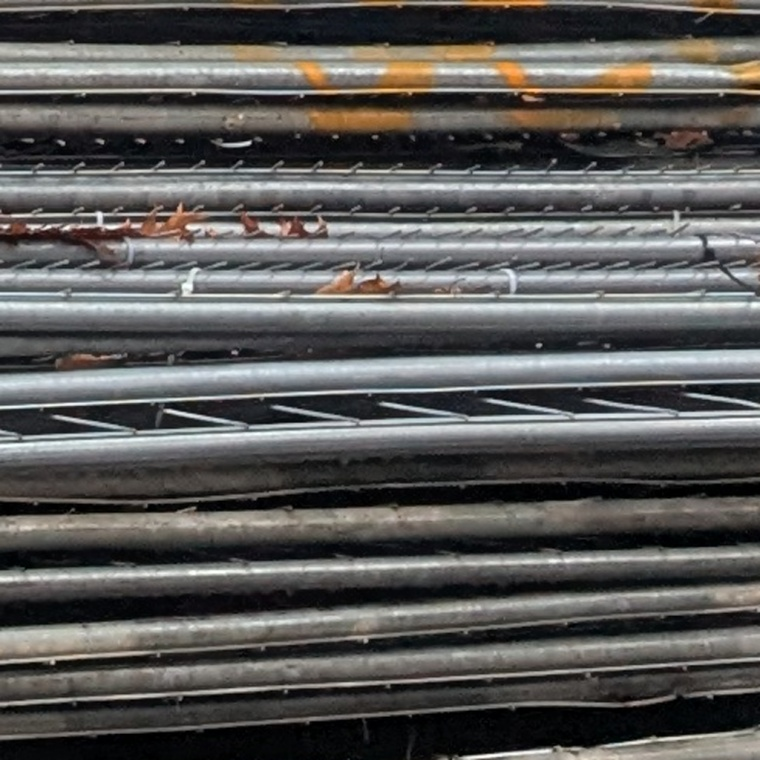
\includegraphics[width=\textwidth]{abbildungen/stufe_T1_hintergrund.jpg}
  \caption{T1 Hintergrund}
\end{subfigure}\hfill
\begin{subfigure}{0.315\textwidth}
  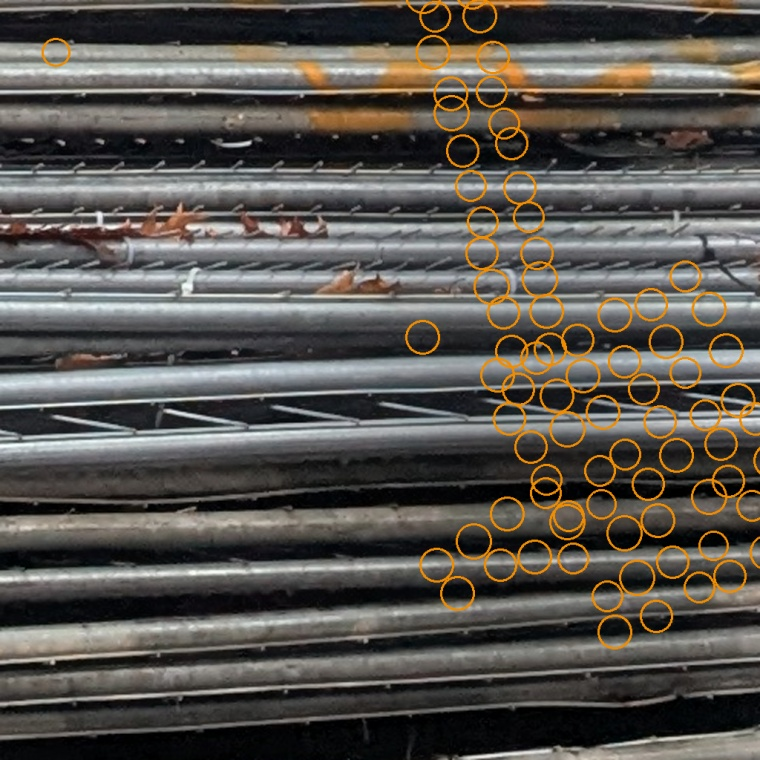
\includegraphics[width=\textwidth]{abbildungen/stufe_T4_layout.jpg}
  \caption{T4 Layout}
\end{subfigure}\hfill
\begin{subfigure}{0.315\textwidth}
  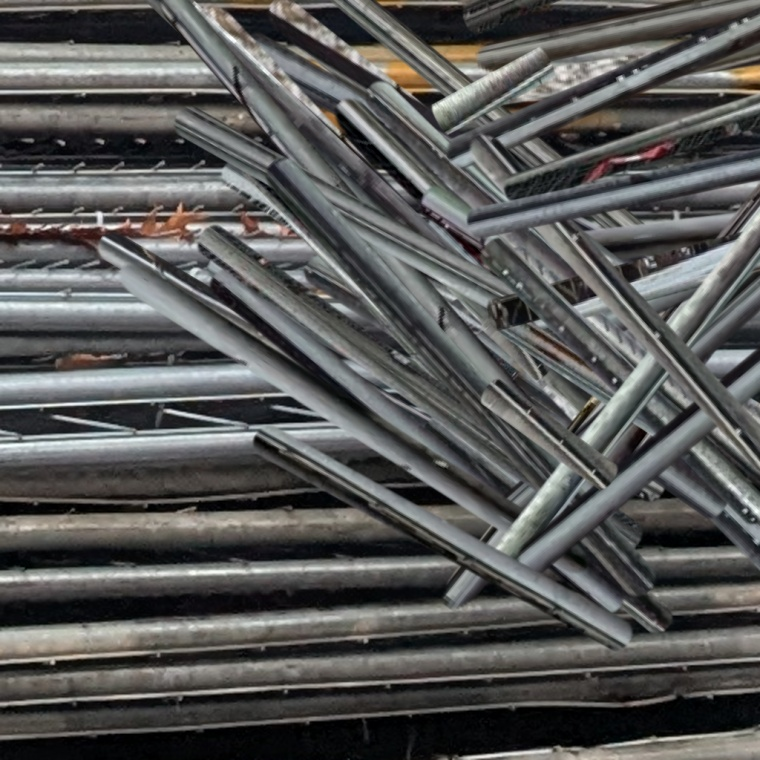
\includegraphics[width=\textwidth]{abbildungen/stufe_T5_schaft.jpg}
  \caption{T5 Rohrschaft}
\end{subfigure}

\vspace{4pt}
\begin{subfigure}{0.315\textwidth}
  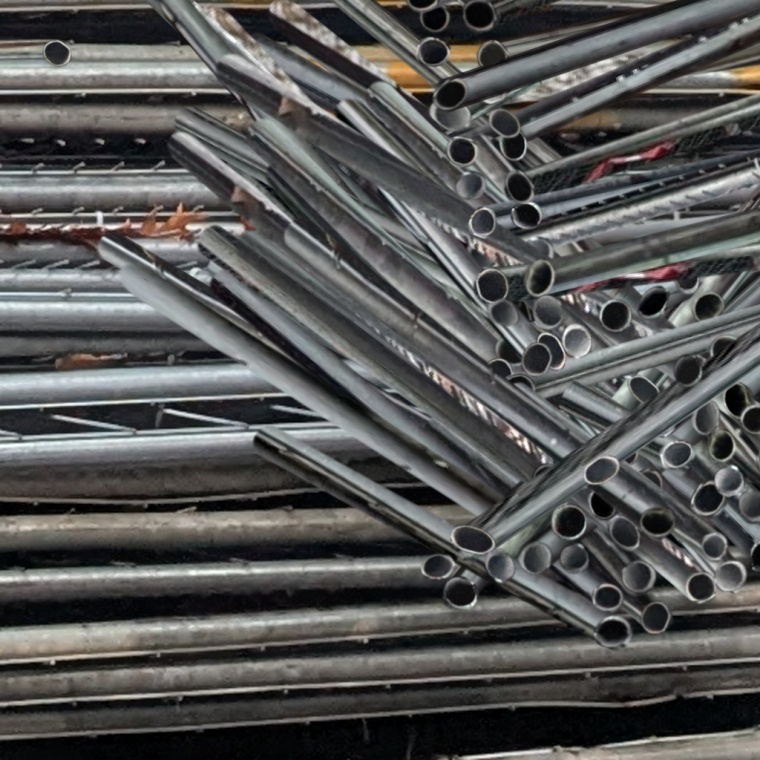
\includegraphics[width=\textwidth]{abbildungen/stufe_T2T3_instanzen.jpg}
  \caption{T2/T3 Instanzen}
\end{subfigure}\hfill
\begin{subfigure}{0.315\textwidth}
  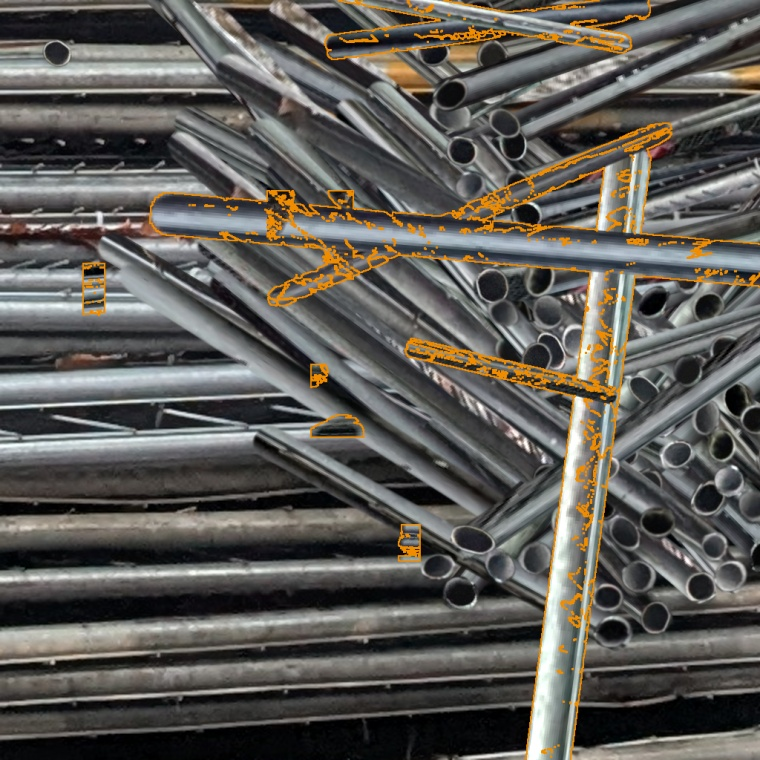
\includegraphics[width=\textwidth]{abbildungen/stufe_T6_okklusion.jpg}
  \caption{T6 Okklusion}
\end{subfigure}\hfill
\begin{subfigure}{0.315\textwidth}
  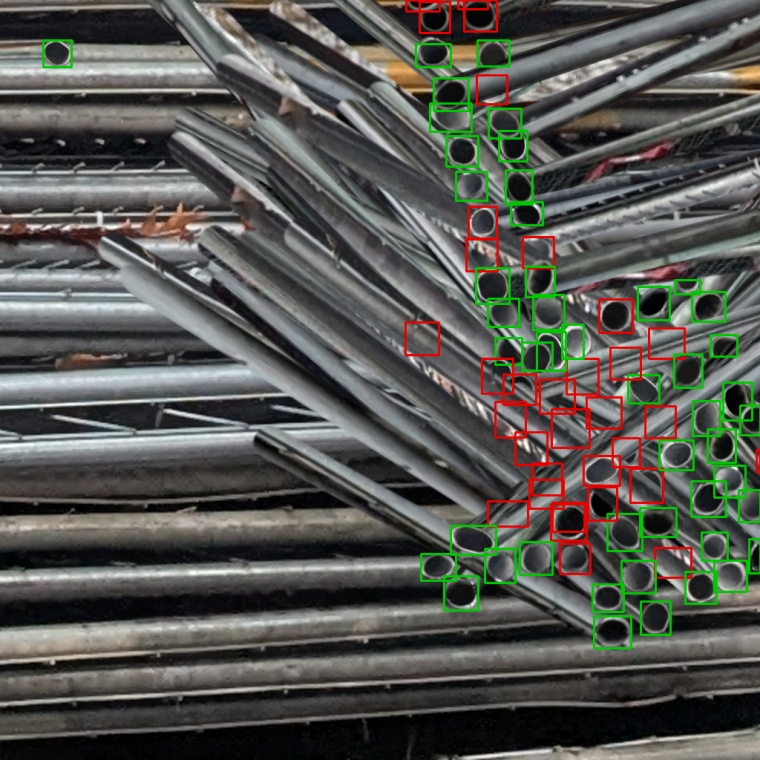
\includegraphics[width=\textwidth]{abbildungen/stufe_T7_sichtbarkeit.jpg}
  \caption{T7 Sichtbarkeit}
\end{subfigure}
\caption[Aufbau eines synthetischen Bildes]{Aufbau eines synthetischen Bildes,
Stufe für Stufe am selben Bild. (a)~Der gewählte Clean Plate nach Zoom,
Ausschnitt und Spiegelung. (b)~Die gezogenen Objektzentren des Layoutmodells
(orange), dazu zwei abgedunkelte Mulden. (c)~Die Rohrschäfte, in paralleler
Richtung und zu 75\,\% ganz hinten gemalt. (d)~Die Stirnflächen mit
Instanzgeometrie und Photometrie -- 82 Instanzen. (e)~Was die Okklusionsstufe
hinzufügt, orange umrandet: sechs quer liegende Stangen und Fremdkörper.
(f)~Das Urteil der Sichtbarkeitsrechnung: grün die 48 vergebenen Labels, rot
die 33 verworfenen Instanzen. Die Einzelstufen T2, T3, T8 und T9 sind in den
Abbildungen~\ref{abb:stufendetail} und~\ref{abb:stufenglobal} im Anhang
vergrößert dargestellt. Zur Lesbarkeit ist ein Bild am oberen Ende des
Größenbereichs gewählt (Basisdurchmesser 44\px{} statt des Medians von
22,5\px) und mit überdurchschnittlicher Verdeckung;
Abbildung~\ref{abb:synthbeispiele} zeigt typische Bilder. Erzeugt mit
\code{paper/tools/fig\_stufen.py}, Seed~302.}
\label{abb:stufen}
\end{figure}

\subsection{Fünf Modellierungsentscheidungen}

\absatz{Maßstabskopplung.} Der Zoomfaktor $z$ wird so gezogen, dass der
Basisdurchmesser im Zielbereich $[12, 44]$\px{} liegt:
\begin{equation}
z \sim \mathcal{U}\!\left[\max\!\left(0{,}55,\;
\tfrac{d_{\min}}{d_{\text{Rohr}}}\right),\;
\min\!\left(2{,}20,\;\tfrac{d_{\max}}{d_{\text{Rohr}}}\right)\right],
\qquad d_{\text{Basis}} = d_{\text{Rohr}} \cdot z .
\label{eq:zoom}
\end{equation}
Objektgröße und Hintergrundmaßstab sind damit \emph{nicht} unabhängig gezogen --
der Kern von Anforderung~A3.

\begin{figure}[htbp]
\centering
\begin{tikzpicture}
\foreach \r/\ok/\sh/\lab in {%
   0.30/1/0/{$d = d_{\text{Rohr}}\cdot z$\\physikalisch korrekt},
   0.46/0/5.9/{$d \neq d_{\text{Rohr}}$\\physikalisch unmöglich}}{
  \begin{scope}[shift={(\sh,0)}]
    \shade[top color=gray!62,bottom color=gray!18] (0,0.28) rectangle (2.25,0.88);
    \draw[gray!65,thin] (0,0.28) rectangle (2.25,0.88);
    \shade[inner color=gray!25,outer color=gray!62] (2.55,0.58) circle (\r);
    \draw[gray!65,semithick] (2.55,0.58) circle (\r);
    \fill[gray!88!black] (2.55,0.58) circle ({\r*0.5});
    \draw[|<->|,thin,blue!60!black] (-0.22,0.28) -- (-0.22,0.88);
    \node[font=\scriptsize,anchor=east,blue!60!black] at (-0.26,0.58)
         {$d_{\text{Rohr}}$};
    \draw[|<->|,thin,orange!85!black] ({2.55+\r+0.16},{0.58-\r})
          -- ({2.55+\r+0.16},{0.58+\r});
    \node[font=\scriptsize,anchor=west,orange!85!black]
         at ({2.55+\r+0.20},0.58) {$d$};
    \ifnum\ok=0
      \draw[red!75!black,very thick] (3.98,0.79) -- (4.34,0.43);
      \draw[red!75!black,very thick] (3.98,0.43) -- (4.34,0.79);
    \fi
    \node[font=\scriptsize,anchor=north,align=center,text width=5.2cm]
         at (1.5,-0.02) {\lab};
  \end{scope}}
\end{tikzpicture}
\caption[Maßstabskopplung]{Die Maßstabskopplung aus
Gleichung~\eqref{eq:zoom}. Links: Die Stirnfläche hat denselben Durchmesser wie
der Schaft, an dem sie sitzt -- es ist dasselbe Rohr. Rechts: Würden Zoom und
Objektgröße unabhängig gezogen, entstünde ein Missverhältnis, das real nicht
vorkommt und dem Netz eine falsche Kontext-Größen-Relation antrainierte.}
\label{abb:zoomkopplung}
\end{figure}

\absatz{Skalierung und Ovalisierung} werden in einem Schritt ausgeführt. Mit
Quelldurchmesser $d_{\text{src}}$, Zieldurchmesser $d$ und gezogenem
Achsverhältnis $\rho$ gilt
\begin{equation}
s_x = \frac{d}{d_{\text{src}}\sqrt{\rho}}, \qquad
s_y = \frac{d\,\sqrt{\rho}}{d_{\text{src}}},
\qquad\text{also}\quad \sqrt{s_x s_y}\, d_{\text{src}} = d .
\label{eq:oval}
\end{equation}
Der geometrische Mittelwert bleibt erhalten -- notwendig, damit die Ovalisierung
die kalibrierte Größenverteilung nicht verschiebt, denn die Realmessung verwendet
mit $\sqrt{\text{Fläche}}$ genau dieses Maß.

\begin{figure}[htbp]
\centering
\begin{tikzpicture}
\foreach \rr/\lab/\sh in {%
   0.66/{$\rho = 0{,}66$ (oblat)}/0,
   1.00/{$\rho = 1$ (Kreis)}/3.6,
   1.30/{$\rho = 1{,}30$ (prolat)}/7.2}{
  \begin{scope}[shift={(\sh,0)}]
    \pgfmathsetmacro{\ax}{1/sqrt(\rr)}
    \pgfmathsetmacro{\by}{sqrt(\rr)}
    \fill[blue!16] (0,0) ellipse ({\ax} and {\by});
    \draw[blue!60!black,semithick] (0,0) ellipse ({\ax} and {\by});
    \draw[gray!55,densely dotted,semithick] (0,0) circle (1);
    \draw[very thick,orange!85!black] ({-\ax},{-\by}) rectangle ({\ax},{\by});
    \node[font=\scriptsize,anchor=north,align=center] at (0,-1.58) {\lab};
  \end{scope}}
\node[font=\scriptsize,anchor=north,align=center] at (3.6,-2.15)
     {gepunktet: Kreis mit Durchmesser $d$ \quad
      \textcolor{orange!85!black}{orange: resultierende Box}};
\end{tikzpicture}
\caption[Ovalisierung]{Ovalisierung nach Gleichung~\eqref{eq:oval}. Alle drei
Ellipsen haben dieselbe Fläche wie der gepunktete Kreis mit Durchmesser $d$, weil
in der Breite mit $1/\sqrt{\rho}$ und in der Höhe mit $\sqrt{\rho}$
skaliert wird: Der geometrische Mittelwert $\sqrt{s_x s_y}\,d_{\text{src}} = d$
bleibt erhalten. Die daraus abgeleitete Box (orange) ändert sich dagegen -- und
genau deren Seitenverhältnis ist die an den Realdaten gemessene Größe.}
\label{abb:ovalisierung}
\end{figure}

\absatz{Farbangleich.} Ein \emph{partieller} Statistiktransfer im Stil von
\textcite{reinhard2001}: Mit Mittelwert und Streuung der Objektpixel
($\mu_i, \sigma_i$) und des lokalen Hintergrunds ($\mu_b, \sigma_b$) gilt je
Farbkanal
\begin{equation}
c' = \mu_i + k\,(c - \mu_i) + \alpha_\mu\,(\mu_b - \mu_i),
\quad
k = 1 + \alpha_\sigma\!\left(\operatorname{clip}\!\left(
\tfrac{\sigma_b}{\sigma_i},\, 0{,}6,\, 1{,}6\right) - 1\right)
\label{eq:harmonize}
\end{equation}
mit $\alpha_\mu \sim \mathcal{U}[0{,}10;\,0{,}45]$ und
$\alpha_\sigma \sim \mathcal{U}[0;\,0{,}35]$. Für
$\alpha_\mu = \alpha_\sigma = 1$ ginge das in den vollständigen
Reinhard-Transfer über -- genau das ist \emph{nicht} gewollt: Ein vollständiger
Angleich ebnete den intrinsischen Albedo-Unterschied zwischen Bohrung und Kranz
ein und zerstörte damit das Objekt. Modelliert wird ausschließlich die
Beleuchtungs- und Weißabgleichdifferenz, nicht die Objektfarbe.

\begin{figure}[htbp]
\centering
\begin{tikzpicture}[x=0.030cm,y=1.9cm]
  \draw[gray!25,fill=gray!25,smooth]
    plot[domain=0:255,samples=110] (\x, {0.85*exp(-((\x-70)/26)^2)})
    -- (255,0) -- (0,0) -- cycle;
  \draw[->,semithick] (0,0) -- (258,0);
  \node[font=\scriptsize,anchor=north] at (215,-0.20) {Grauwert};
  \foreach \g in {0,50,100,150,200,250}
    \draw[semithick] (\g,0) -- (\g,-0.030) node[below,font=\scriptsize] {\g};
  \draw[red!70!black,thick,dotted,smooth]
    plot[domain=0:255,samples=150] (\x, {1.18*exp(-((\x-70)/12)^2)});
  \draw[very thick,blue!60!black,smooth]
    plot[domain=0:255,samples=150]
    (\x, {exp(-((\x-60)/16)^2) + 0.9*exp(-((\x-155)/20)^2)});
  \draw[very thick,orange!85!black,densely dashed,smooth]
    plot[domain=0:255,samples=150]
    (\x, {exp(-((\x-46)/16)^2) + 0.9*exp(-((\x-141)/20)^2)});
  \draw[dashed,gray!55] (70,0) -- (70,1.34);
  \node[font=\scriptsize,gray!40!black,anchor=south,fill=white,inner sep=1pt]
       at (70,1.32) {$\mu_b$};
  \draw[dashed,gray!55] (105,0) -- (105,1.34);
  \node[font=\scriptsize,gray!40!black,anchor=south,fill=white,inner sep=1pt]
       at (105,1.32) {$\mu_i$};
  \draw[->,>=stealth,orange!85!black,thick] (105,1.13) -- (91,1.13);
  \node[font=\scriptsize,orange!85!black,anchor=south,inner sep=1pt,
        fill=white] at (97,1.16) {$\alpha_\mu(\mu_b - \mu_i)$};
  \node[font=\scriptsize,blue!60!black,anchor=south,fill=white,inner sep=1pt]
       at (58,1.03) {Bohrung};
  \node[font=\scriptsize,blue!60!black,anchor=south,fill=white,inner sep=1pt]
       at (158,0.93) {Kranz};
  % Legende rechts neben der Achse
  \begin{scope}[shift={(272,0)}]
    \draw[very thick,blue!60!black] (0,1.15) -- (22,1.15);
    \node[font=\scriptsize,anchor=west] at (26,1.15) {Objekt, vorher};
    \draw[very thick,orange!85!black,densely dashed] (0,0.90) -- (22,0.90);
    \node[font=\scriptsize,anchor=west] at (26,0.90) {teilweise angeglichen};
    \draw[thick,red!70!black,dotted] (0,0.65) -- (22,0.65);
    \node[font=\scriptsize,anchor=west] at (26,0.65) {vollständiger Angleich};
    \fill[gray!25] (0,0.34) rectangle (22,0.46);
    \node[font=\scriptsize,anchor=west] at (26,0.40) {lokaler Hintergrund};
  \end{scope}
\end{tikzpicture}
\caption[Partieller Farbangleich]{Partieller Farbangleich nach
Gleichung~\eqref{eq:harmonize}. Die Grauwertverteilung des Objekts ist
zweigipfelig: dunkle Bohrung und heller Kranz. Der Angleich verschiebt sie um
$\alpha_\mu(\mu_b - \mu_i)$ in Richtung des lokalen Hintergrunds, hält die
beiden Gipfel aber auseinander. Ein vollständiger Angleich
($\alpha_\mu = \alpha_\sigma = 1$, gepunktet) zöge sie auf die
Hintergrundverteilung zusammen und zerstörte damit den Albedo-Unterschied, der
das Objekt überhaupt erkennbar macht.}
\label{abb:farbangleich}
\end{figure}

\absatz{Rauschschätzung.} Das lokale Rauschniveau wird als Streuung eines
Hochpassrests geschätzt \parencite[vgl.][]{immerkaer1996} -- mit einem
Medianfilter als Tiefpass, weil er Kanten weniger verschmiert:
\begin{equation}
\hat{\sigma} = \operatorname{std}\!\big(g - \operatorname{median}_{3\times3}(g)\big),
\quad
\sigma_{\text{Rausch}} = \max\!\big(0{,}5,\; \hat{\sigma} \cdot
\mathcal{U}[0{,}5;\,1{,}25]\big).
\label{eq:noise}
\end{equation}

\iffalse

\begin{figure}[htbp]
\centering
\begin{tikzpicture}
\begin{scope}[xscale=1.62,yscale=1.55]
  \draw[->,semithick] (-0.08,0) -- (4.95,0);
  \draw[->,semithick] (-0.08,0) -- (-0.08,1.62);
  \node[font=\scriptsize,anchor=east,xscale=0.617,yscale=0.645]
       at (-0.14,1.45) {$g$};
  \draw[thick,red!70!black,dotted] (0.000,0.2551) -- (0.145,0.2541) -- (0.290,0.2271) -- (0.435,0.2004) --
    (0.580,0.1963) -- (0.725,0.2056) -- (0.870,0.2566) -- (1.015,0.2891) --
    (1.160,0.2462) -- (1.305,0.2303) -- (1.450,0.2628) -- (1.595,0.2713) --
    (1.740,0.2442) -- (1.885,0.2194) -- (2.030,0.2754) -- (2.175,0.5450) --
    (2.320,1.0254) -- (2.465,1.2601) -- (2.610,1.2605) -- (2.755,1.2525) --
    (2.900,1.2680) -- (3.045,1.3042) -- (3.190,1.3232) -- (3.335,1.3629) --
    (3.480,1.3736) -- (3.625,1.3221) -- (3.770,1.2653) -- (3.915,1.3052) --
    (4.060,1.3554) -- (4.205,1.3465) -- (4.350,1.3070) -- (4.495,1.3068) --
    (4.640,1.3038);
  \draw[very thick,orange!85!black] (0.000,0.2743) -- (0.145,0.2501) -- (0.290,0.2277) -- (0.435,0.2131) --
    (0.580,0.1776) -- (0.725,0.2131) -- (0.870,0.2549) -- (1.015,0.2549) --
    (1.160,0.2100) -- (1.305,0.2100) -- (1.450,0.2790) -- (1.595,0.2790) --
    (1.740,0.2586) -- (1.885,0.2476) -- (2.030,0.2476) -- (2.175,0.3065) --
    (2.320,1.2658) -- (2.465,1.2658) -- (2.610,1.2702) -- (2.755,1.2254) --
    (2.900,1.2702) -- (3.045,1.2720) -- (3.190,1.3559) -- (3.335,1.3877) --
    (3.480,1.3877) -- (3.625,1.3598) -- (3.770,1.3312) -- (3.915,1.3312) --
    (4.060,1.3711) -- (4.205,1.3711) -- (4.350,1.3362) -- (4.495,1.2955) --
    (4.640,1.3362);
  \draw[very thick,blue!60!black] (0.000,0.2501) -- (0.145,0.2743) -- (0.290,0.2277) -- (0.435,0.1776) --
    (0.580,0.2131) -- (0.725,0.1694) -- (0.870,0.2549) -- (1.015,0.3589) --
    (1.160,0.2100) -- (1.305,0.1996) -- (1.450,0.2898) -- (1.595,0.2790) --
    (1.740,0.2586) -- (1.885,0.1744) -- (2.030,0.2476) -- (2.175,0.3065) --
    (2.320,1.2658) -- (2.465,1.3378) -- (2.610,1.2205) -- (2.755,1.2702) --
    (2.900,1.2254) -- (3.045,1.3559) -- (3.190,1.2720) -- (3.335,1.3970) --
    (3.480,1.3877) -- (3.625,1.3598) -- (3.770,1.1705) -- (3.915,1.3312) --
    (4.060,1.3711) -- (4.205,1.3842) -- (4.350,1.2507) -- (4.495,1.3362) --
    (4.640,1.2955);
\end{scope}
\node[font=\scriptsize,anchor=north] at (3.9,-0.30)
     {(a) Profil über eine Kante};
\begin{scope}[shift={(8.55,1.15)},font=\scriptsize]
  \draw[very thick,blue!60!black] (0,0.62) -- (0.42,0.62);
  \node[anchor=west] at (0.5,0.62) {$g$};
  \draw[very thick,orange!85!black] (0,0.31) -- (0.42,0.31);
  \node[anchor=west] at (0.5,0.31) {$\operatorname{median}_{3\times3}(g)$};
  \draw[thick,red!70!black,dotted] (0,0) -- (0.42,0);
  \node[anchor=west] at (0.5,0) {Gauß-Tiefpass};
\end{scope}
\begin{scope}[shift={(0,-2.65)},xscale=1.62]
  \draw[semithick,gray!55] (-0.08,0) -- (4.95,0);
  \begin{scope}[yscale=4.2]
    \draw[thick,red!70!black,dotted] (0.000,-0.0050) -- (0.145,0.0202) -- (0.290,0.0006) -- (0.435,-0.0228) --
    (0.580,0.0167) -- (0.725,-0.0362) -- (0.870,-0.0017) -- (1.015,0.0698) --
    (1.160,-0.0362) -- (1.305,-0.0307) -- (1.450,0.0270) -- (1.595,0.0077) --
    (1.740,0.0144) -- (1.885,-0.0450) -- (2.030,-0.0277) -- (2.175,-0.2385) --
    (2.320,0.2404) -- (2.465,0.0777) -- (2.610,-0.0400) -- (2.755,0.0177) --
    (2.900,-0.0427) -- (3.045,0.0517) -- (3.190,-0.0511) -- (3.335,0.0342) --
    (3.480,0.0142) -- (3.625,0.0377) -- (3.770,-0.0948) -- (3.915,0.0260) --
    (4.060,0.0157) -- (4.205,0.0377) -- (4.350,-0.0564) -- (4.495,0.0294) --
    (4.640,-0.0083);
    \draw[very thick,orange!85!black] (0.000,-0.0242) -- (0.145,0.0242) -- (0.290,0.0000) -- (0.435,-0.0354) --
    (0.580,0.0354) -- (0.725,-0.0436) -- (0.870,0.0000) -- (1.015,0.1040) --
    (1.160,0.0000) -- (1.305,-0.0104) -- (1.450,0.0108) -- (1.595,0.0000) --
    (1.740,0.0000) -- (1.885,-0.0732) -- (2.030,0.0000) -- (2.175,0.0000) --
    (2.320,0.0000) -- (2.465,0.0720) -- (2.610,-0.0497) -- (2.755,0.0449) --
    (2.900,-0.0449) -- (3.045,0.0839) -- (3.190,-0.0839) -- (3.335,0.0093) --
    (3.480,0.0000) -- (3.625,0.0000) -- (3.770,-0.1607) -- (3.915,0.0000) --
    (4.060,0.0000) -- (4.205,0.0131) -- (4.350,-0.0855) -- (4.495,0.0407) --
    (4.640,-0.0407);
    \draw[<->,red!70!black,thin] (2.06,-0.2385) -- (2.06,0.2404);
  \end{scope}
  \node[font=\scriptsize,red!70!black,anchor=south,xscale=0.617,
        fill=white,inner sep=1pt] at (2.06,1.02) {$\pm19$ Grauwerte};
  \node[font=\scriptsize,orange!85!black,anchor=west,xscale=0.617,
        inner sep=1pt] at (2.62,0.66) {Median an der Kante: genau 0};
  \draw[orange!85!black,thin] (2.56,0.60) -- (2.36,0.06);
  \node[font=\scriptsize,anchor=east,xscale=0.617] at (-0.10,0.0)
       {$g-\hat g$};
\end{scope}
\node[font=\scriptsize,anchor=north] at (3.9,-3.85) {(b) Hochpassrest};
\end{tikzpicture}
\caption[Rauschschätzung mit Medianfilter]{Warum ein Medianfilter als Tiefpass
dient. (a)~Grauwertprofil über eine Materialkante mit 6,5 Grauwerten Rauschen;
der Median folgt der Kante, ein Gauß-Tiefpass rundet sie ab. (b)~Der
Hochpassrest, aus dem $\hat\sigma$ nach Gleichung~\eqref{eq:noise} geschätzt
wird: Beim Gauß-Tiefpass erzeugt die Kante allein einen Ausschlag von $\pm19$
Grauwerten -- das Dreifache der Rauschamplitude --, der in strukturreichen
Ausschnitten in die Schätzung eingeht; beim Median ist der Rest an der Kante
exakt null. Werte aus einer Simulation mit festem Seed.}
\label{abb:rauschschaetzung}
\end{figure}

\fi

\absatz{Layoutmodell.} Pro Cluster mit Basisdurchmesser $d_0$ liegen die
Objektzentren auf einer gescherten, verrauschten Gitterpackung
\begin{equation}
p_{ij} = i\,s_1\,\mathbf{e}_1 + j\,s_2\,\mathbf{e}_2 + \mathbf{c}
+ \boldsymbol{\epsilon}_{ij},
\qquad \boldsymbol{\epsilon}_{ij} \sim \mathcal{N}\!\big(\mathbf{0},
(0{,}17\,d_0)^2 \mathbf{I}\big),
\label{eq:layout}
\end{equation}
mit Gitterabständen von mindestens einem Objektdurchmesser -- Rohrzentren
können sich nicht durchdringen -- und Basisrichtungen $\mathbf{e}_1$,
$\mathbf{e}_2$, deren eingeschlossener Winkel die Scherung des Gitters bestimmt.
Die Bereiche der Einzelparameter stehen in Tabelle~\ref{tab:parameter}; sie sind
nicht gemessen, sondern iterativ so eingestellt, dass die erzeugte Anordnung die
in Tabelle~\ref{tab:kalibrierung} gegenübergestellten Kenngrößen der Realbilder
trifft. Das Clusterzentrum $\mathbf{c}$ darf außerhalb der
Leinwand liegen, sodass angeschnittene Objekte am Bildrand entstehen (Befund~9).

\begin{figure}[htbp]
\centering
\begin{tikzpicture}[x=1cm,y=1cm]
% ================= (a) Gitterkonstruktion =================
\begin{scope}
  \pgfmathsetmacro{\cx}{0.62}
  \pgfmathsetmacro{\cy}{3.00}
  \pgfmathsetmacro{\ea}{-100}
  \pgfmathsetmacro{\eb}{-16}
  \pgfmathsetmacro{\sa}{0.98}
  \pgfmathsetmacro{\sb}{1.06}
  \pgfmathsetmacro{\rd}{0.44}
  % gezogene Lagen
  \foreach \i in {0,1}{\foreach \j in {0,1,2}{
    \pgfmathsetmacro{\ix}{\cx + \i*\sa*cos(\ea) + \j*\sb*cos(\eb)}
    \pgfmathsetmacro{\iy}{\cy + \i*\sa*sin(\ea) + \j*\sb*sin(\eb)}
    \pgfmathsetmacro{\jx}{0.085*(mod(7*\i+3*\j,5)-2)}
    \pgfmathsetmacro{\jy}{0.085*(mod(11*\i+5*\j,5)-2)}
    \fill[blue!14] ({\ix+\jx},{\iy+\jy}) circle (\rd);
    \draw[blue!60!black,thin] ({\ix+\jx},{\iy+\jy}) circle (\rd);}}
  % ideale Gitterpunkte darueber
  \foreach \i in {0,1}{\foreach \j in {0,1,2}{
    \pgfmathsetmacro{\ix}{\cx + \i*\sa*cos(\ea) + \j*\sb*cos(\eb)}
    \pgfmathsetmacro{\iy}{\cy + \i*\sa*sin(\ea) + \j*\sb*sin(\eb)}
    \draw[gray!75!black,thin] ({\ix-0.07},{\iy-0.07}) -- ({\ix+0.07},{\iy+0.07})
                              ({\ix-0.07},{\iy+0.07}) -- ({\ix+0.07},{\iy-0.07});}}
  % Basisvektoren
  \draw[->,>=stealth,very thick,orange!85!black] (\cx,\cy)
    -- ({\cx+\sa*cos(\ea)},{\cy+\sa*sin(\ea)});
  \node[font=\scriptsize,orange!85!black,anchor=east,inner sep=1pt,
        fill=white]
    at ({\cx+0.62*\sa*cos(\ea)-0.10},{\cy+0.62*\sa*sin(\ea)}) {$s_1\mathbf{e}_1$};
  \draw[->,>=stealth,very thick,blue!65!black] (\cx,\cy)
    -- ({\cx+\sb*cos(\eb)},{\cy+\sb*sin(\eb)});
  \node[font=\scriptsize,blue!65!black,anchor=south,inner sep=2pt]
    at ({\cx+0.58*\sb*cos(\eb)},{\cy+0.58*\sb*sin(\eb)}) {$s_2\mathbf{e}_2$};
  % eingeschlossener Winkel
  \draw[gray!60!black,thin] ({\cx+0.50*cos(\ea)},{\cy+0.50*sin(\ea)})
    arc[start angle=\ea, end angle=\eb, radius=0.50];
  \node[font=\scriptsize,gray!35!black,inner sep=1pt,fill=white]
    at ({\cx+0.62*cos(-50)},{\cy+0.62*sin(-50)}) {$55^\circ\!-\!125^\circ$};
  % Clusterzentrum
  \fill[black] (\cx,\cy) circle (1.6pt);
  \node[font=\scriptsize,anchor=south east,inner sep=1pt]
    at ({\cx+0.10},{\cy+0.03}) {$\mathbf{c}$};
  % Rauschen an einem Punkt hervorheben
  \pgfmathsetmacro{\hx}{\cx + \sa*cos(\ea) + \sb*cos(\eb)}
  \pgfmathsetmacro{\hy}{\cy + \sa*sin(\ea) + \sb*sin(\eb)}
  \pgfmathsetmacro{\hjx}{0.085*(mod(7*1+3*1,5)-2)}
  \pgfmathsetmacro{\hjy}{0.085*(mod(11*1+5*1,5)-2)}
  \draw[red!70!black,densely dashed,thin] (\hx,\hy) circle (0.34);
  \draw[->,>=stealth,red!70!black,semithick]
    (\hx,\hy) -- ({\hx+\hjx},{\hy+\hjy});
  \node[font=\scriptsize,red!70!black,anchor=north,inner sep=1pt]
    at ({\hx},{\hy-0.50}) {$\boldsymbol{\epsilon}_{ij}$};
  \node[font=\scriptsize,gray!40!black,anchor=north west,align=left]
    at (-0.28,0.88)
    {$\times$\; ideales Gitter\\$\circ$\; gezogene Lage\\
     \textcolor{red!70!black}{gestrichelt: $2\sigma$ von
     $\boldsymbol{\epsilon}_{ij}$}};
  \node[font=\scriptsize,anchor=north] at (1.45,-0.10) {(a) Konstruktion};
\end{scope}
% ================= (b) Leinwand =================
\begin{scope}[shift={(3.72,0)}]
  % Geisterkreise: das Gitter setzt sich ausserhalb der Leinwand fort
  \foreach \i in {0,1,2,3,4}{\foreach \j in {0,1,2}{
    \pgfmathsetmacro{\jx}{0.05*(mod(7*\i+3*\j,5)-2)}
    \pgfmathsetmacro{\jy}{0.05*(mod(11*\i+5*\j,5)-2)}
    \pgfmathsetmacro{\bx}{5.62 + \i*0.50*cos(-152) + \j*0.62*cos(-64) + \jx}
    \pgfmathsetmacro{\by}{3.44 + \i*0.50*sin(-152) + \j*0.62*sin(-64) + \jy}
    \draw[gray!45,thin] (\bx,\by) circle (0.145);}}
  \begin{scope}
    \clip (0,0.98) rectangle (5.30,3.62);
    \foreach \i in {0,1,2,3}{\foreach \j in {0,1}{
      \pgfmathsetmacro{\jx}{0.05*(mod(5*\i+2*\j,5)-2)}
      \pgfmathsetmacro{\jy}{0.05*(mod(13*\i+7*\j,5)-2)}
      \pgfmathsetmacro{\ax}{1.22 + \i*0.47*cos(-14) + \j*0.60*cos(72) + \jx}
      \pgfmathsetmacro{\ay}{1.92 + \i*0.47*sin(-14) + \j*0.60*sin(72) + \jy}
      \fill[blue!14] (\ax,\ay) circle (0.145);
      \draw[blue!60!black,thin] (\ax,\ay) circle (0.145);}}
    \foreach \i in {0,1,2,3,4}{\foreach \j in {0,1,2}{
      \pgfmathsetmacro{\jx}{0.05*(mod(7*\i+3*\j,5)-2)}
      \pgfmathsetmacro{\jy}{0.05*(mod(11*\i+5*\j,5)-2)}
      \pgfmathsetmacro{\bx}{5.62 + \i*0.50*cos(-152) + \j*0.62*cos(-64) + \jx}
      \pgfmathsetmacro{\by}{3.44 + \i*0.50*sin(-152) + \j*0.62*sin(-64) + \jy}
      \fill[blue!14] (\bx,\by) circle (0.145);
      \draw[blue!60!black,thin] (\bx,\by) circle (0.145);
      \ifdim\bx cm>5.02cm
        \draw[very thick,orange!85!black]
          ({\bx-0.145},{\by-0.145}) rectangle ({\bx+0.145},{\by+0.145});
      \fi}}
  \end{scope}
  \draw[dashed,gray!70] (0,0.98) rectangle (5.30,3.62);
  \node[font=\scriptsize,gray!45!black,anchor=north west] at (0.10,3.55)
       {Leinwand $1024 \times 1024$};
  \node[font=\scriptsize,orange!85!black,anchor=south west] at (0.10,1.04)
       {orange: angeschnittene Boxen};
  \fill[black] (5.62,3.44) circle (1.6pt);
  \node[font=\scriptsize,anchor=south,inner sep=3pt] at (5.62,3.44) {$\mathbf{c}$};
  \node[font=\scriptsize,anchor=north] at (2.65,-0.10) {(b) zwei Cluster};
\end{scope}
\end{tikzpicture}
\caption[Layoutmodell]{Das Layoutmodell aus Gleichung~\eqref{eq:layout}.
(a)~Konstruktion eines Clusters: Die Objektzentren liegen auf einem gescherten
Gitter mit den Basisrichtungen $\mathbf{e}_1$ und $\mathbf{e}_2$, deren
eingeschlossener Winkel zwischen $55^\circ$ und $125^\circ$ liegt; die
Gitterabstände liegen bei $s_1 \in [0{,}98;\,1{,}60]\,d_0$ und
$s_2 \in [0{,}98;\,1{,}85]\,d_0$. Auf jede ideale Gitterlage ($\times$) wirkt
zusätzlich das Rauschen $\boldsymbol{\epsilon}_{ij}$, sodass die gezogene Lage
($\circ$) um typischerweise $0{,}17\,d_0$ davon abweicht -- ohne diesen Term
entstünden sichtbar künstliche Reihen. (b)~Pro Bild werden ein bis drei solche
Cluster gezogen. Weil das Clusterzentrum $\mathbf{c}$ außerhalb der Leinwand
liegen darf, ragt ein Teil des Gitters (grau) über den Bildrand hinaus; von
diesen Objekten bleibt nur der sichtbare Teil, und ihre Boxen werden am
Bildrand abgeschnitten. In \code{test} sind 5,8\,\% der Labels angeschnitten.}
\label{abb:layout}
\end{figure}

\section{Sichtbarkeitsrechnung und Labelerzeugung}
\label{sec:sichtbarkeit}

Kein Copy-Paste-Generator darf Labels blind vergeben: Ein Objekt, das nach dem
Einfügen zu 95\,\% verdeckt ist, hat kein sinnvolles Label mehr. Für
\emph{jede} Instanz wird daher die exakte Sichtbarkeit berechnet. Grundlage ist
die Alpha-Kompositionsregel von \textcite{porter1984}: Wird Instanz $i$ von allen
später gemalten Schichten $j$ überlagert, so ist ihr sichtbarer Anteil
\begin{equation}
\alpha_i^{\text{sichtbar}} = \alpha_i \prod_{j > i} \big(1 - \alpha_j\big),
\qquad
v_i = \frac{\textstyle\sum \alpha_i^{\text{sichtbar}}}{\textstyle\sum \alpha_i},
\label{eq:sichtbarkeit}
\end{equation}
wobei das Produkt über \emph{alle} später gemalten Schichten läuft --
einschließlich anderer Profile, Rohrschäfte und Fremdkörper. Die Buchhaltung
läuft über die beschnittenen Alphafenster in Malreihenfolge, ist also exakt und
nicht approximiert.

Daraus folgen vier Regeln, die dieselben sind, nach denen \code{val} und
\code{test} annotiert wurden (Anforderung~A5): Ein Label wird verworfen, wenn die
Sichtbarkeit unter 30\,\% liegt (30\,801 Objekte, 17,8\,\% der gerenderten) --
unter 30\,\% sichtbarer Fläche wäre das Objekt auch für einen menschlichen
Annotator nicht mehr sicher identifizierbar, und \emph{kein} Label macht dieselbe
Bildstelle zum korrekten harten Negativ; wenn weniger als 15\,\% der Fläche im
Bild liegen (3\,846 Objekte); oder wenn die sichtbare Box unter 5\px{} fällt
(228 Objekte). Vergeben wird stets die \emph{modale} Box, also der sichtbare
Umriss. Insgesamt werden 34\,875 der 173\,100 gerenderten Instanzen verworfen
(20,1\,\%). Diese Zahl ist kein Verlust, sondern der Ertrag der Stufe: Sie
markiert genau jene Bildstellen, an denen ein naiver Generator ein falsches Label
gesetzt hätte.

\section{Der erzeugte Datensatz}
\label{sec:datensatz}

Es entstehen 6000 Bilder zu $1024\times1024$ Pixeln, davon 583 Negativbilder
(9,7\,\%), mit 136\,384 gelabelten Objekten (22,7 pro Bild) aus 173\,100
gerenderten Instanzen. Die mittlere Sichtbarkeit der gelabelten Objekte beträgt
90,0\,\%, 30,1\,\% von ihnen sind teilverdeckt. Der Objektdurchmesser liegt bei
p05/Median/p95 = 11,6/22,5/39,9\px, das Seitenverhältnis bei
p10/Median/p90 = 0,77/1,00/1,40.

Der wichtigste Qualitätsnachweis ist nicht der optische Eindruck, sondern der
Vergleich der erzeugten mit der gemessenen Statistik
(Tabelle~\ref{tab:kalibrierung}).

\begin{table}[htbp]
\centering
\caption[Kalibrierung gegen die Realmessung]{Kalibrierung des Layoutmodells
gegen die Realmessung ($n = 174$). Alle Abstände in Objektdurchmessern.}
\label{tab:kalibrierung}
\footnotesize
\begin{tabular}{@{}lccc@{}}
\toprule
\textbf{Kenngröße} & \textbf{real \code{val}} & \textbf{real \code{test}} &
\textbf{synthetisch (Ist)} \\
\midrule
NN-Abstand p10 / Median / p90 & 0,86 / 1,09 / 1,78 &
0,83 / 1,24 / 2,51 & \textbf{0,84 / 1,17 / 1,87} \\
berührt den NN ($< 1{,}2\,\Oe$) & 61,4\,\% & 46,5\,\% & \textbf{53,6\,\%} \\
Nachbarn innerhalb $5\,\Oe$ (Median) & 10 & 10 & \textbf{13} \\
Größenverhältnis zum NN (Median) & 1,05 & 1,05 &
\textbf{1,05} (per Konstruktion) \\
\bottomrule
\end{tabular}
\end{table}

Die synthetische Verteilung liegt bei allen vier Kenngrößen zwischen oder nahe
bei den beiden realen Messungen. Die einzige systematische Abweichung ist die
Nachbarzahl: Die synthetischen Cluster sind dichter (13 statt 10 Nachbarn
innerhalb $5\,\Oe$, im Maximum 61 statt 20). Das ist bewusst so belassen -- eine
höhere Dichte im Training ist eine Robustheitsreserve, weil sie den Detektor auf
schwierigere Szenen vorbereitet als die, die er zur Inferenzzeit vorfindet. Die
umgekehrte Abweichung wäre gefährlich gewesen.

\section{Nachweis der Anforderungen}
\label{sec:nachweis}

Anforderung~\textbf{A1} ist erfüllt, weil die Box nach jeder
Instanztransformation aus der transformierten Alphamaske neu bestimmt wird und
die boxverfälschenden Operationen zur Trainingszeit auf~0 stehen.
\textbf{A2}: Objektgrößen 12--44\px{} aus der Realmessung, Leinwandgröße gleich
der Trainingsauflösung. \textbf{A3}: Maßstabskopplung, Schaft hinter jeder
Stirnfläche, parallele Schaftrichtung, Tiefenmodell 75/25, volle Rotation.
\textbf{A4}: S1 Alphamaske und Kantenweichzeichnung, S2 partieller Farbangleich,
S3 flächentreue Skalierung und Unschärfeangleich, S4 lokal geschätzter
Rauschangleich, S5 JPEG-Requantisierung, S6 Schlagschatten und physikalische
Verdeckung. \textbf{A5}: modale Boxen und dieselben Verwerfungsregeln wie bei der
Handannotation -- allerdings nur \emph{annähernd}, wie
Abschnitt~\ref{sec:boxversatz} zeigt: Die Generatorboxen folgen der
$\alpha > 0{,}5$-Kontur und fallen damit um 1,2 bis 2,5\px{} kleiner aus als die
Handannotation. \textbf{A6}: Tabelle~\ref{tab:parameter} mit Sollbereich und
gemessenem Ist-Anteil je Transformation, sieben Werte ausdrücklich als Annahme
gekennzeichnet.

Die Anforderungen sind damit \emph{formal} erfüllt. Das sagt nichts darüber aus,
ob die einzelnen Maßnahmen \emph{wirken} -- die Erfüllung einer
Entwurfsanforderung ist kein empirischer Nachweis. Diese Unterscheidung wird in
Kapitel~\ref{kap:auswertung} durch die Messung des Sim-to-Real-Abstands und die
Okklusionsablation adressiert und in Abschnitt~\ref{sec:tragend} bilanziert.

\chapter{Training und Trainingszeit-Augmentierung}
\label{kap:trainingszeit}

\section{Aufbau}
\label{sec:trainingsaufbau}

\absatz{Datenaufteilung.} Trainiert wird auf den 6000 synthetischen Bildern,
validiert auf dem \emph{realen} \code{val}-Bild (88 Objekte). Das ist eine
bewusste Entscheidung: Die Modellauswahl muss auf der Zieldomäne erfolgen, sonst
wählt man das Modell, das am besten zu den eigenen Renderartefakten passt.
\code{test} (86 Objekte) berührt Training und Modellauswahl nie und dient
ausschließlich der Endbewertung. Ein vierter Split \code{sval} aus 400
synthetischen Bildern mit anderem Seed dient allein der Messung des
Sim-to-Real-Abstands (Abschnitt~\ref{sec:simtoreal}).

\absatz{Modellwahl.} Als Baseline dient \code{yolo11s} mit 9,4~Millionen
Parametern. Die Größe folgt aus der Datenlage: Der Datensatz hat eine Klasse und
nur neun zugrunde liegende Objektinstanzen, die Formvielfalt ist klein, die
nötige Modellkapazität damit ebenfalls; die \enquote{nano}-Variante verliert bei
12--40\px{} großen Objekten Rückruf, größere Varianten würden die synthetischen
Eigenheiten eher memorieren. Ausgangspunkt sind COCO-vortrainierte Gewichte: Die
vortrainierten Low-Level-Filter sind domänenunabhängig \parencite{yosinski2014},
und \textcite{hinterstoisser2018} zeigen den Nutzen explizit für synthetische
Trainingsdaten. Die \emph{Familie} yolo11 war zunächst konservativ gewählt
(ausgereifte Implementierung, bekannte Kopfstruktur P3/P4/P5) und nicht belegt;
Abschnitt~\ref{sec:p2} prüft mit zwei YOLO26-Varianten nach, was ein feinerer
Detektionskopf bringt. Alle verglichenen Modelle haben auf P3/P4/P5 dieselben
Schrittweiten, sodass die Auflösungsargumentation und die Ergebnisse von
Abschnitt~\ref{sec:imgsz} unverändert gültig bleiben.

\absatz{Eingabegröße.} \code{imgsz}=1024, identisch zur Leinwandgröße des
Generators. Damit durchlaufen die synthetischen Bilder \emph{keine} Skalierung,
und die Objekte erreichen das Netz mit exakt der Pixelgröße, für die die Pipeline
ausgelegt ist (Anforderung~A2). Bei 640\px{} wären sie nur 7--27\px{} groß und
lägen teils unter der Auflösung der P3-Ebene.

\absatz{Optimierung.} AdamW \parencite{loshchilov2019} mit
$\text{lr}_0 = 10^{-3}$, Endlernrate 1\,\% davon, Kosinusabfall
\parencite{loshchilov2017sgdr}, drei Aufwärmepochen, Weight Decay $5\cdot10^{-4}$,
Batch~16, Mixed Precision \parencite{micikevicius2018}, fester Seed und
deterministische Kernel. AdamW ist explizit gesetzt statt \code{auto}, weil es
bei kleinen Datensätzen schneller konvergiert und robust gegenüber der
Lernratenwahl ist -- wichtig, weil kein Budget für eine Lernratensuche vorhanden
ist. Die Verlustgewichte bleiben auf den Standardwerten
(\code{box}\,7,5 / \code{cls}\,0,5): Eine Erhöhung des Boxgewichts wäre bei
kleinen Objekten denkbar, ohne separaten Abstimmungssplit aber nicht belegbar.
Das Budget beträgt 60 Epochen mit Early Stopping nach 20 Epochen ohne
Verbesserung auf dem realen \code{val}-Bild; der Hauptlauf endete dadurch nach
30 Epochen mit dem besten Modell aus Epoche~10.

\section{Augmentierungsparameter zur Trainingszeit}
\label{sec:trainparam}

Die abgeschalteten Parameter sind genauso begründungspflichtig wie die aktiven --
ein auf Null gesetzter Standardwert ist eine Entscheidung.

Aktiv sind Mosaic (immer, in den letzten zehn Epochen abgeschaltet), Skalierung
$0{,}6$--$1{,}4$, Translation, horizontale und vertikale Spiegelung sowie
HSV-Variation (Ton 0,015, Sättigung 0,7, Helligkeit 0,4). Abgeschaltet sind
\code{degrees}, \code{shear} und \code{perspective}, weil Bildrotation
achsparallele Boxen aufbläht -- bei $10^\circ$ um 15,8\,\% der Kantenlänge, was
die Überlappung mit der korrekten Box auf 0,745 senkt
(Abschnitt~\ref{sec:boxrotation}) --, sowie \code{mixup} und \code{cutmix}, die
Bildinhalte bei erhaltenen Labels überlagern und damit Geisterobjekte mit vollem
Boxlabel erzeugen \parencite{zhang2018mixup,yun2019cutmix}: Bei dicht gepackten
20\px-Objekten überwiegt der Labelkonflikt. \code{erasing} entfällt, weil es in
der Werkzeugkette nur bei der Klassifikation wirkt, und \code{copy\_paste},
weil es Segmentierungsmasken benötigt -- beides übernimmt der Generator
physikalisch korrekt. Die vollständige Tabelle mit Begründung je Parameter steht
im Anhang (Tabelle~\ref{tab:trainaug}).

Die beiden Augmentierungsschichten wirken bei der Objektgröße multiplikativ: Der
Generator erzeugt $[12, 44]$\px, die Trainingsskalierung multipliziert mit
$[0{,}6;\,1{,}4]$, sodass das Netz effektiv Objekte von
$12 \cdot 0{,}6 = 7{,}2$ bis $44 \cdot 1{,}4 = 61{,}6$\px{} sieht. Diese Spanne
deckt nach unten die Objektgrößen bei niedriger
Inferenzauflösung und nach oben jene bei starker Hochskalierung ab -- also den
gesamten in Abschnitt~\ref{sec:imgsz} durchmusterten Bereich. Der untere Rand von
7,2\px{} liegt knapp unter dem Stride der feinsten Ebene; ein kleinerer Wert für
\code{scale} hätte den Bereich sinnvoll auflösbarer Objekte verlassen.

\section{Trainingsverlauf}
\label{sec:trainingsverlauf}


Die Lernkurven zeigen den Sim-to-Real-Abstand in zeitlicher Form: Der
Trainingsverlust fällt über alle 30 Epochen monoton, die Metrik auf dem realen
\code{val}-Bild ist ab Epoche~10 flach. Ab dort verbessert das
Modell ausschließlich seine Anpassung an Eigenschaften der synthetischen Daten,
die in der Zieldomäne nicht gelten. Genau deshalb ist es methodisch notwendig,
das beste Modell über den \emph{realen} Validierungssplit auszuwählen: Eine
synthetische Validierung wählte das Modell aus der letzten Epoche und damit das
am stärksten überangepasste.

\chapter{Auswertung}
\label{kap:auswertung}

\section{Metriken und Bewertungsprotokoll}
\label{sec:metriken}

Eine Detektion gilt als Treffer, wenn ihre Box eine Ground-Truth-Box mit einer
\emph{Intersection over Union} von mindestens $t$ überdeckt; jede
Ground-Truth-Box kann höchstens einmal getroffen werden. Daraus folgen
\emph{Precision} $P$, \emph{Recall} $R$ und deren harmonisches Mittel $F_1$;
berichtet wird stets das beste $F_1$ über alle Konfidenzschwellen samt der
zugehörigen Schwelle $c^*$ -- der Betriebspunkt, den man in einer Anwendung
wählen würde. \emph{mAP} ist die Fläche unter der Precision-Recall-Kurve
\parencite{everingham2010}; \mAPfifty{} verwendet $t = 0{,}5$, \mAPseven{}
$t = 0{,}75$ und \mAPall{} den Mittelwert über $t = 0{,}50; \dots; 0{,}95$ nach
COCO-Konvention \parencite{lin2014coco}. Der \emph{Zählfehler} ist die für die
Anwendung eigentlich relevante Größe; er ist nicht aus mAP ableitbar, weil er
zusätzlich davon abhängt, ob sich Falsch-Positive und Falsch-Negative
kompensieren.

Die Bewertung erfolgt über eine eigene Implementierung, weil Zählfehler, mittlere
Treffer-IoU und der $F_1$-optimale Betriebspunkt gebraucht werden -- Größen, die
die Standardfunktion der Werkzeugkette nicht ausgibt. Zur Absicherung wurde sie
gegen die Referenzimplementierung geprüft: \code{val} 0,886/0,597 gegen
0,897/0,599 und \code{test} 0,888/0,437 gegen 0,891/0,424
(\mAPfifty{}/\mAPall{}); die Abweichung von maximal 1,3\PP{} ist durch
Detailunterschiede in der AP-Interpolation erklärbar.

\section{Hauptergebnis und Sim-to-Real-Abstand}
\label{sec:hauptergebnis}

\begin{table}[htbp]
\centering
\caption[Hauptergebnis]{Ergebnis des besten Modells bei nativem Maßstab.
Die Zählung steht voran, weil sie die Zielgröße der Anwendung ist
(Abschnitt~\ref{sec:metriken}); $c^*$ ist die $F_1$-optimale
Konfidenzschwelle.}
\label{tab:hauptergebnis}
\footnotesize
\resizebox{\textwidth}{!}{%
\begin{tabular}{@{}lrrrrrrrrr@{}}
\toprule
\textbf{Split} & \textbf{Zählung} & \textbf{Zählfehler} &
\mAPfifty{} & \mAPseven{} & \mAPall{} & \textbf{bestes $F_1$} &
$c^*$ & $P$\,/\,$R$ & \textbf{mittl.\ IoU} \\
\midrule
\code{val} (real)  & 86/88 & \textbf{2,3\,\%} & 0,886 & 0,793 & 0,597 & 0,862 & 0,336 & 0,872\,/\,0,852 & 0,824 \\
\code{test} (real) & 84/86 & \textbf{2,3\,\%} & 0,888 & 0,320 & 0,437 & 0,894 & 0,263 & 0,905\,/\,0,884 & 0,748 \\
\code{sval} (synth.) & 7128/7248 & 1,7\,\% & 0,982 & 0,935 & 0,828 & 0,964 & 0,450 & 0,972\,/\,0,956 & 0,899 \\
\bottomrule
\end{tabular}}
\end{table}

Ein ausschließlich auf synthetischen Bildern trainiertes Modell zählt auf
echten, nie im Training gesehenen Aufnahmen 86 statt 88 und 84 statt 86 Objekte
-- ein \textbf{Zählfehler von 2,3\,\%} auf beiden realen Aufnahmen und damit die
Antwort auf die Aufgabenstellung. Gefunden werden dabei etwa 88--89\,\% der
Objekte bei vergleichbarer Precision. Bei der auf \code{val} gewählten Inferenzauflösung steigt
\mAPfifty{} auf \code{test} auf 0,928, mit Test-Time-Augmentation auf 0,934.

Der auffällige Unterschied zwischen den Splits -- \mAPseven{} 0,793 auf
\code{val}, aber nur 0,320 auf \code{test} bei praktisch identischem
\mAPfifty{} -- ist kein Widerspruch, sondern der in
Abschnitt~\ref{sec:ioukleinobjekt} beschriebene Empfindlichkeit der IoU bei
kleinen Objekten: Die Objekte in \code{test} sind kleiner (Median 19,6 gegen
27,4\px), und die mittlere Treffer-IoU bestätigt den Unterschied direkt (0,748
gegen 0,824). Die Objektgröße ist allerdings nur ein Teil der Erklärung -- der
größere Teil ist ein \emph{systematischer Größenversatz zwischen
Generatorlabel und Handannotation}, der in
Abschnitt~\ref{sec:boxversatz} aufgeschlüsselt wird. \mAPall{} ist bei dieser
Objektgröße daher weniger ein Maß für die Detektionsqualität als für
Pixelauflösung und Labelkonvention -- eine Feststellung, die für alle folgenden
Tabellen gilt. Ein Qualitativbild der Detektionen zeigt
Abbildung~\ref{abb:qualitativ} im Anhang.


\absatz{Sim-to-Real-Abstand.}\label{sec:simtoreal}
Der Split \code{sval} besteht aus 400 synthetischen Bildern derselben Pipeline
mit anderem Seed und trennt damit zwei Fragen: \emph{Kann das Modell die Aufgabe
überhaupt?} und \emph{überträgt es sich auf echte Bilder?} Der Abstand beträgt
$0{,}982 - 0{,}886/0{,}888 = \mathbf{9{,}6}$ bzw.\ $\mathbf{9{,}5}$\PP{}
\mAPfifty{}; bei \mAPall{} sind es 23,1 (\code{val}) bzw.\ 39,1 (\code{test})
Prozentpunkte. Er ist damit \textbf{klein genug}, dass das Verfahren praktisch
funktioniert, und \textbf{groß genug}, um zu belegen, dass das Netz \emph{nicht}
bloß Einfügeartefakte gelernt hat: Wäre die Pipeline an einer der Signaturen
S1--S6 durchlässig, so wäre \code{sval} nahezu perfekt ($>0{,}99$) und die realen
Bilder katastrophal. Genau dieses Muster tritt nicht auf -- der einzige
\emph{direkte} empirische Hinweis darauf, dass die Anti-Abkürzungs-Maßnahmen
greifen, und ein Indiz, kein Beweis.

\section{Experiment 1: die Inferenzauflösung}
\label{sec:imgsz}

Die Inferenzauflösung ist der einzige hier untersuchte Parameter, der nach dem
Training noch frei ist, und deshalb der einzige, dessen Wert gemessen statt
begründet wird. Gemustert werden neun Stufen zwischen 640 und 2464\px{} sowie
der native Maßstab, gemessen auf der \code{yolo11s}-Baseline. Ausgewählt wird
die Stufe mit dem höchsten \mAPall{} auf \code{val}, und zwar ausschließlich
dort; der so gefundene Wert wird unverändert auf beide Splits angewandt -- eine
Wahl je Split wäre eine Hyperparameterselektion auf dem Testsatz und würde
dessen Zahlen wertlos machen. Das Kriterium ist bewusst \mAPall{} und nicht
\mAPfifty{}, weil es die Lokalisierungsgüte mitbewertet; es stand vor den Läufen
fest und gilt unverändert für alle in dieser Arbeit ausgewerteten Modelle. Für
die Baseline fallen beide Metriken auseinander: \mAPfifty{} ist bei 1600 am
höchsten, \mAPall{} bei 1920 (Tabelle~\ref{tab:imgszvoll} im Anhang); gewählt
wurde daher 1920.

\begin{table}[htbp]
\centering
\caption[Sweep der Inferenzauflösung]{Auszug aus dem Sweep der
Inferenzauflösung. Nativer Maßstab ist 2464 (\code{val}) bzw.\ 1600
(\code{test}); der vollständige Sweep umfasst neun Stufen je Split.}
\label{tab:imgsz}
\footnotesize
\begin{tabular}{@{}lrrrrr@{}}
\toprule
\code{imgsz} & \code{val} \mAPfifty{} & \code{val} $R$ &
\code{test} \mAPfifty{} & \code{test} $R$ & \code{val} pred/gt \\
\midrule
640  & 0,435 & 0,398 & 0,524 & 0,465 & 50/88 \\
960  & 0,852 & 0,773 & 0,889 & 0,826 & 74/88 \\
1280 & 0,887 & 0,841 & 0,900 & 0,849 & 84/88 \\
1600 & \textbf{0,904} & 0,898 & 0,888 & 0,884 & 98/88 \\
1920 & 0,893 & 0,909 & \textbf{0,928} & 0,895 & 100/88 \\
2464 & 0,886 & 0,852 & 0,927 & 0,895 & 86/88 \\
\bottomrule
\end{tabular}
\end{table}

Von \code{imgsz}~640 auf 1600 steigt \mAPfifty{} auf \code{val} von 0,435 auf
0,904 -- eine Verdopplung und mit 47\PP{} der größte gemessene Einzeleffekt der
Arbeit, größer als jede einzelne Entscheidung in der Augmentierungspipeline. Die
Erklärung ist rein geometrisch und wurde in
Abschnitt~\ref{sec:ioukleinobjekt} vorhergesagt: Bei \code{imgsz}~640 wird das
2459\px{} breite \code{val}-Bild um den Faktor 0,26 verkleinert, die Objekte
schrumpfen von 20--36 auf 5--9\px{} und unterschreiten die Schrittweite~8 der
feinsten Detektionsebene. Der Rückruf bricht entsprechend auf 0,398 ein: Das
Modell \emph{findet} die Objekte nicht mehr, es lokalisiert sie nicht bloß
schlechter.

Bemerkenswert ist, dass das Optimum \emph{nicht} am nativen Maßstab liegt. Für
\code{test} (1600\px{} breit) ist eine Hochskalierung um Faktor 1,2--1,5 spürbar
besser als der native Maßstab (0,928 gegen 0,888). Der Grund liegt in der
Trainingsverteilung: Der Generator erzeugt Objekte mit Median 22,5\px{},
\code{test} hat nur 19,6\px{} Median -- eine leichte Hochskalierung schiebt die
Testobjekte in die Mitte der Trainingsverteilung. Daraus folgt die Empfehlung,
\emph{nicht} auf den nativen Maßstab zu skalieren, sondern so, dass die erwartete
Objektgröße im Netzeingang etwa dem Median der Trainingsverteilung entspricht --
hier rund 22\px. Der Objektgrößenbereich des Generators und die
Inferenzauflösung sind damit \emph{nicht} unabhängig voneinander wählbar. Die
übrigen Inferenzparameter sind dagegen unkritisch: Der NMS-Schwellwert bewegt zwischen
0,3 und 0,9 nur 3\PP{} (benachbarte Rohrenden haben mindestens 0,85 Durchmesser
Abstand, ihre Boxen überlappen also kaum), \code{max\_det} ist ab 100 gesättigt
(bei 50 dagegen katastrophal: Zählung 50/88), und FP16 liefert bitidentische
Ergebnisse. Test-Time-Augmentation bringt $+2{,}1$\PP{} auf \code{val} und
$+0{,}6$ auf \code{test} bei doppeltem Rechenaufwand \parencite{shanmugam2021} --
für eine Zählanwendung ohne Echtzeitanforderung lohnend.

\section{Experiment 2: Wie viel Verdeckung in den Trainingsdaten?}
\label{sec:ablation}

Dies ist das zentrale Augmentierungsexperiment: Die Okklusionserzeugung ist die
aufwendigste Einzelstufe der Pipeline -- sie erfordert die Okkluder-Bibliothek,
das Tiefenmodell und die exakte Sichtbarkeitsrechnung. Zahlt sich der Aufwand
messbar aus?

\absatz{Versuchsaufbau.} Drei Datensätze unterscheiden sich \emph{ausschließlich}
im Verdeckungsgrad; alles andere ist identisch (derselbe Seed, 3000 Bilder,
dieselben Hyperparameter, 30 Epochen). Arm~\textbf{A0} hat keine quer liegenden
Stangen, keine Fremdkörper und keinen Schaft, der vor einer Stirnfläche kreuzt;
\textbf{A1} ist die Baseline aus Kapitel~\ref{kap:pipeline}; \textbf{A2} hat in
jedem Bild Stangen, mehr Fremdkörper und mehr quer vor dem Stapel liegende Rohre.
Der Rohrschaft \emph{hinter} der Stirnfläche bleibt in allen Armen erhalten -- er
ist physikalische Randbedingung, keine Augmentierung. Die Kontrolle ist besser als
bei einer gewöhnlichen Datensatz-Ablation: Weil der Seed identisch ist, rendern
alle drei Arme \textbf{genau dieselben 86\,617 Instanzen an denselben
Positionen}. Der einzige Unterschied ist, wie viel davon verdeckt wird -- und als
Folge, wie viele Labels die Sichtbarkeitsregel verwirft.

\begin{table}[htbp]
\centering
\caption[Okklusionsablation]{Okklusionsablation: erzeugte Datensätze (links) und
Ergebnis bei nativem Maßstab (rechts). Alle sechs Metrikspalten sind über die
drei Arme \textbf{monoton}.}
\label{tab:ablation}
\footnotesize
\resizebox{\textwidth}{!}{%
\begin{tabular}{@{}lrrr|rrrrrr@{}}
\toprule
\textbf{Arm} & \textbf{Labels} & \textbf{Sichtb.} & \textbf{teilverd.} &
\code{val} \mAPfifty{} & \code{val} \mAPall{} &
\code{test} \mAPfifty{} & \code{test} \mAPall{} & \code{test} $F_1$ &
\code{test} Zählung \\
\midrule
A0 ohne     & 82\,950 & 0,977 & 12,0\,\% & 0,888 & 0,606 & 0,899 & 0,418 & 0,896 & 77/86 \\
A1 Baseline & 68\,281 & 0,902 & 29,9\,\% & 0,924 & 0,609 & 0,911 & 0,452 & 0,904 & 80/86 \\
A2 stark    & 55\,833 & 0,852 & 40,7\,\% & \textbf{0,930} & \textbf{0,620} &
\textbf{0,919} & \textbf{0,454} & \textbf{0,910} & \textbf{81/86} \\
\bottomrule
\end{tabular}}
\end{table}

Drei Befunde. \emph{(1) Der Effekt ist monoton:} Von A0 zu A2 steigen
\mAPfifty{} um 2,0\PP{} und \mAPall{} um 3,6\PP{} auf dem unberührten Testbild,
und zwar in allen sechs Metrikspalten und über alle drei Stufen in derselben
Richtung. \emph{(2) Der Gewinn entsteht gegen einen Verlust an Supervision:} A2
hat durch die stärkere Verdeckung \textbf{32,7\,\% weniger Labels} als A0
(55\,833 gegen 82\,950 bei identischer Bildzahl und identischen gerenderten
Instanzen). Der Okklusionsvorteil überkompensiert also einen deutlichen Verlust an
Trainingssignal -- der stärkste Einzelbeleg dafür, dass die Okklusionsstufe kein
Beiwerk ist: Wären die zusätzlichen Labels wertvoller als die zusätzliche
Schwierigkeit, müsste A0 gewinnen. \emph{(3) Ohne Verdeckung ist die Aufgabe zu
leicht:} A0 erreichte sein bestes Modell bereits in Epoche~3 und verbesserte sich
in den folgenden 20 Epochen nicht mehr, A1 und A2 verbesserten sich bis zur
letzten Epoche~30 durchgehend.

\absatz{Einordnung und Einschränkungen.} Der Befund ist mit den Ergebnissen zu
Cutout und Random Erasing verträglich
\parencite{devries2017cutout,zhong2020erasing}, geht aber über sie hinaus: Dort
wird Bildinhalt gelöscht und das Label beibehalten, hier verdeckt ein Objekt mit
eigener Textur, und das Label wird bei zu starker Verdeckung entfernt -- die
entstehenden Beispiele sind damit sowohl schwierigere Positive als auch korrekte
harte Negative. Drei Vorbehalte bleiben. Erstens liegt der Effekt
\emph{innerhalb} des Konfidenzintervalls von $\pm 0{,}05$ (\code{val}) bzw.\
$\pm 0{,}04$ (\code{test}); belastbar ist nicht die einzelne Differenz, sondern
die \emph{Konsistenz} -- dieselbe Richtung in drei Metriken $\times$ zwei Splits
$\times$ drei Stufen, was bei reinem Rauschen unwahrscheinlich wäre. Nicht monoton
verläuft \mAPseven{} auf \code{val} (0,812 / 0,760 / 0,775); die Aussage betrifft
das Finden der Objekte, nicht die Präzision der Boxen. Zweitens sind Labelzahl und
Okklusionsanteil nicht entkoppelt -- mehr Verdeckung heißt zwangsläufig mehr
verworfene Labels. Drittens waren A1 und A2 nach 30 Epochen nicht auskonvergiert;
die Aussage ist konservativ, aber nicht abgeschlossen.

\section{Experiment 3: der P2-Detektionskopf}
\label{sec:p2}

\subsection{Frage und Versuchsaufbau}

Abschnitt~\ref{sec:ioukleinobjekt} hat die Auflösungsgrenze quantifiziert: Ein
Objekt mit Durchmesser $d$ belegt auf einer Ebene mit Schrittweite $S$ im Mittel
$\pi d^2/(4S^2)$ Gitterzellen, und unterhalb von $d < S\sqrt{2}$ existieren
Lagen, bei denen \emph{kein} Zellzentrum im Objekt liegt. Für die feinste
Standardebene P3 ($S = 8$) liegt diese Grenze bei 11,3\px{} -- genau im Bereich
der hier auftretenden Objektgrößen. Die Architekturseite bietet dafür eine
direkte Gegenmaßnahme: einen zusätzlichen Detektionskopf auf der Ebene P2 mit
Schrittweite~4 (Abbildung~\ref{abb:pyramide}). Dieses Experiment prüft, was er
bringt und was er kostet.

Verglichen werden \code{yolo26s} (Ebenen P3--P5) und \code{yolo26s-p2}
(Ebenen P2--P5). Bewusst \emph{nicht} verglichen wird mit der yolo11s-Baseline:
Ein Vergleich über Modellfamilien hinweg vermischte den Effekt der Kopfstruktur
mit dem der Familie. Beide Modelle werden auf demselben Datensatz, mit denselben
Hyperparametern und demselben Budget trainiert und mit demselben
Bewertungsframework gemessen; \code{yolo26s-p2} startet von den
\code{yolo26s}-Gewichten, damit auch die Initialisierung vergleichbar ist.

\subsection{Was der zusätzliche Kopf architektonisch bedeutet}

Der Unterschied liegt allein im Neck und im Kopf. Die
Standardkonfiguration führt den Aufwärtspfad des Feature-Pyramid-Netzwerks
\parencite{lin2017fpn} bis P3 und schickt von dort einen Abwärtspfad über P4 zu
P5; die \code{-p2}-Variante setzt den Aufwärtspfad um eine Stufe fort,
verknüpft ihn mit der P2-Karte des Backbones und startet den Abwärtspfad
entsprechend eine Ebene tiefer. Der Detektionskopf erhält damit vier statt drei
Eingänge. Weil die Eingangsbreite des Kopfes seine internen Kanalzahlen bestimmt
und der neue, feinste Eingang schmaler ist als der bisherige, hat die
\code{-p2}-Variante sogar \emph{weniger} Parameter als das Basismodell --
sie ist kein größeres, sondern ein \emph{feiner aufgelöstes} Netz.

\begin{table}[htbp]
\centering
\caption[Kennzahlen der beiden Varianten]{Kennzahlen der beiden Varianten. Die
Prädiktionspositionen und Gittergrößen gelten für eine Eingabe von
$1024\times1024$; GFLOPs und Parameter sind die Werte der tatsächlich
trainierten Modelle (eine Klasse), Speicher und Zeit die gemessenen Werte des
Trainingslaufs bei \code{imgsz}=1024 und Batch~16.}
\label{tab:p2kennzahlen}
\footnotesize
\begin{tabularx}{\textwidth}{@{}Xrr@{}}
\toprule
\textbf{Kenngröße} & \textbf{\code{yolo26s}} & \textbf{\code{yolo26s-p2}} \\
\midrule
Detektionsebenen (Schrittweite) & 8 / 16 / 32 & \textbf{4} / 8 / 16 / 32 \\
Gittergrößen & $128^2$ / $64^2$ / $32^2$ & $\mathbf{256^2}$ / $128^2$ / $64^2$ / $32^2$ \\
Prädiktionspositionen & 21\,504 & \textbf{87\,040} \quad($\times 4{,}05$) \\
Kanalzahl der Kopfeingänge & 128 / 256 / 512 & 64 / 128 / 256 / 512 \\
Netzschichten & 260 & 329 \\
Parameter & 9\,948\,638 & 9\,663\,464 \quad($-2{,}9\,\%$) \\
GFLOPs (bei $640^2$) & 22,7 & 26,6 \quad($+17\,\%$) \\
GPU-Speicher im Training & 15,1\,GB & 35,3\,GB \quad($\times 2{,}3$) \\
Zeit je Epoche & 138\,s & 173\,s \quad($\times 1{,}26$) \\
bestes Modell in Epoche & 5 & 22 \\
\bottomrule
\end{tabularx}
\end{table}

Tabelle~\ref{tab:p2kennzahlen} zeigt die Asymmetrie der Kosten. Die
\textbf{Prädiktionspositionen} vervierfachen sich, weil die neue Ebene mit
$256 \times 256 = 65\,536$ Positionen allein mehr enthält als P3, P4 und P5
zusammen ($16\,384 + 4\,096 + 1\,024 = 21\,504$). Der Rechenaufwand wächst
dagegen nur um 17\,\%, weil die zusätzlichen Blöcke auf der feinsten Ebene
schmal sind. Der \textbf{Speicherbedarf} wächst am stärksten -- um Faktor 2,3 --,
denn er wird von den Aktivierungen dominiert, und die skalieren mit der
räumlichen Auflösung: Eine Merkmalskarte auf P2 hat viermal so viele Positionen
wie eine auf P3. Das ist der eigentliche Preis der Variante und der Grund, warum
sie nicht der Standard ist.

\subsection{Die Rechnung: Kandidatenzellen je Objekt}

Der Nutzen lässt sich vor jedem Training abschätzen. Nach
Gleichung~\eqref{eq:zellen} beträgt die erwartete Zahl der Gitterzellen, deren
Zentrum in ein kreisförmiges Objekt vom Durchmesser $d$ fällt und die damit
überhaupt als positive Zuweisung in Frage kommen,
$\mathbb{E}[N] = \pi d^2/(4S^2)$. Der Übergang von $S = 8$ auf $S = 4$
vervierfacht diesen Wert. Tabelle~\ref{tab:p2zellen} setzt ihn für die
tatsächlich auftretenden Objektgrößen ein.

\begin{table}[htbp]
\centering
\caption[Kandidatenzellen je Objekt]{Erwartete Zahl der Gitterzellen, deren
Zentrum in das Objekt fällt, nach Gleichung~\eqref{eq:zellen}. Die Spalte
\enquote{min} nennt den ungünstigsten Fall über alle Lagen des Objektzentrums im
Gitter.}
\label{tab:p2zellen}
\footnotesize
\begin{tabular}{@{}rlrrrr@{}}
\toprule
$d$ (px) & Bedeutung & \multicolumn{2}{c}{P3 ($S=8$)} &
\multicolumn{2}{c}{P2 ($S=4$)} \\
 & & Mittel & min & Mittel & min \\
\midrule
11,6 & p05 des synthetischen Datensatzes & 1,7 & 1 & 6,6 & 4 \\
12,2 & kleinstes Objekt in \code{test}   & 1,8 & 1 & 7,3 & 4 \\
19,6 & Median \code{test}                & 4,7 & 4 & 18,9 & 16 \\
22,5 & Median des synthetischen Datensatzes & 6,2 & 4 & 24,9 & 21 \\
27,4 & Median \code{val}                 & 9,2 & 8 & 36,9 & 32 \\
\bottomrule
\end{tabular}
\end{table}

\begin{figure}[htbp]
\centering
\begin{tikzpicture}[x=1cm,y=1cm]
  % ---------------- P3: Zellen 8 px = 0.5 cm ------------------------------
  \begin{scope}
    \draw[step=0.5,gray!45,thin] (0,0) grid (4,4);
    \draw[gray!70] (0,0) rectangle (4,4);
    \fill[blue!14] (2,2) circle (0.703);
    \draw[blue!65!black,thick] (2,2) circle (0.703);
    \foreach \x in {1.75,2.25}{\foreach \y in {1.75,2.25}{
      \fill[red!80!black] (\x,\y) circle (0.055);}}
    \foreach \x in {0.25,0.75,...,3.8}{\foreach \y in {0.25,0.75,...,3.8}{
      \fill[gray!45] (\x,\y) circle (0.028);}}
    \node[below,align=center,font=\small] at (2,-0.25)
         {\textbf{P3}, Schrittweite 8\\4 Kandidatenzellen};
  \end{scope}
  % ---------------- P2: Zellen 4 px = 0.25 cm -----------------------------
  \begin{scope}[shift={(5.4,0)}]
    \draw[step=0.25,gray!35,very thin] (0,0) grid (4,4);
    \draw[gray!70] (0,0) rectangle (4,4);
    \fill[blue!14] (2,2) circle (0.703);
    \draw[blue!65!black,thick] (2,2) circle (0.703);
    \foreach \x in {1.625,1.875,2.125,2.375}{
      \foreach \y in {1.625,1.875,2.125,2.375}{
        \fill[red!80!black] (\x,\y) circle (0.045);}}
    \foreach \p in {{1.375,1.875},{1.375,2.125},{2.625,1.875},{2.625,2.125},
                    {1.875,1.375},{2.125,1.375},{1.875,2.625},{2.125,2.625}}{
      \fill[red!80!black] (\p) circle (0.045);}
    \foreach \x in {0.125,0.375,...,3.9}{\foreach \y in {0.125,0.375,...,3.9}{
      \fill[gray!40] (\x,\y) circle (0.02);}}
    \node[below,align=center,font=\small] at (2,-0.25)
         {\textbf{P2}, Schrittweite 4\\24 Kandidatenzellen};
  \end{scope}
\end{tikzpicture}
\caption[Kandidatenzellen auf P3 und P2]{Warum ein feineres Gitter hilft.
Dargestellt ist ein Bildbereich von $64\times64$ Pixeln mit einem Objekt von
22,5\px{} Durchmesser -- dem Median des synthetischen Datensatzes. Punkte sind
Gitterzellenzentren, rot markiert sind jene, die in das Objekt fallen und damit
als positive Labelzuweisung in Frage kommen. In der gezeichneten Lage sind es 4
gegen 24; über alle Lagen des Objektzentrums gemittelt 6,2 gegen 24,9
(Tabelle~\ref{tab:p2zellen}). Bei einem ankerfreien Kopf ist diese Zahl das
Trainingssignal, das je Objekt zur Verfügung steht.}
\label{abb:p2zellen}
\end{figure}

Zwei Ablesungen sind entscheidend. Erstens: Für die kleinsten real auftretenden
Objekte steht auf P3 im ungünstigsten Fall nur \emph{eine} Kandidatenzelle zur
Verfügung, auf P2 sind es vier. Ein Objekt, dessen Zuweisung an einer einzigen
Zelle hängt, ist gegenüber der Diskretisierung des Gitters maximal empfindlich --
genau das Problem, das die Small-Target-Aware Label Assignment von YOLO26 auf der
Verlustseite mildert. Zweitens ist der Vorteil \emph{größenabhängig}: Bei
27,4\px{} bietet schon P3 neun Zellen, die zusätzlichen 37 auf P2 ändern wenig.
Die Erwartung lautet also nicht \enquote{P2 hilft}, sondern \enquote{P2 hilft
dort, wo die Objekte klein sind} -- und diese Erwartung ist prüfbar.

\subsection{Ergebnis}

\begin{table}[htbp]
\centering
\caption[Ergebnis des P2-Vergleichs]{Ergebnis des P2-Vergleichs. Oben nativer
Maßstab, unten bei der je Modell nach \mAPall{} auf \code{val} gewählten
Auflösung (\code{yolo26s}: 1600, \code{yolo26s-p2}: 1920); \code{test} blieb an
der Auswahl unbeteiligt. Fett ist je Spalte der bessere Wert -- die beiden
Modelle werden von der Zielgröße \emph{Zählfehler} und von \mAPfifty{}
\textbf{gegenläufig} geordnet (Abschnitt~\ref{sec:p2zaehlung}).}
\label{tab:p2ergebnis}
\footnotesize
\resizebox{\textwidth}{!}{%
\begin{tabular}{@{}lrrrrrrrr@{}}
\toprule
\textbf{Modell} & \code{test} \textbf{Zählung} &
\code{test} \textbf{Zählfehler} & \code{val} \mAPfifty{} &
\code{test} \mAPfifty{} & \code{test} \mAPseven{} & \code{test} \mAPall{} &
\code{test} $F_1$ & \code{test} $P$ / $R$ \\
\midrule
\multicolumn{9}{@{}l}{\itshape nativer Maßstab}\\
\code{yolo26s}    & \textbf{83/86} & \textbf{3,5\,\%} & 0,931 & 0,905 & 0,333 & 0,427 & 0,888 & 0,904 / 0,872 \\
\code{yolo26s-p2} & 79/86 & 8,1\,\% & \textbf{0,936} & \textbf{0,941} &
\textbf{0,387} & \textbf{0,450} & \textbf{0,933} & \textbf{0,975} / \textbf{0,895} \\
\midrule
\multicolumn{9}{@{}l}{\itshape bei der auf \code{val} gewählten \code{imgsz}}\\
\code{yolo26s} (1600)    & \textbf{83/86} & \textbf{3,5\,\%} & 0,939 & 0,905 & -- & 0,427 & 0,888 & 0,904 / 0,872 \\
\code{yolo26s-p2} (1920) & 81/86 & 5,8\,\% & \textbf{0,940} & \textbf{0,947} & -- &
\textbf{0,449} & \textbf{0,934} & \textbf{0,963} / \textbf{0,907} \\
\bottomrule
\end{tabular}}
\end{table}

Die theoretische Erwartung bestätigt sich: Bei praktisch identischer
Parameterzahl erreicht \code{yolo26s-p2} auf dem unberührten Testbild
\mAPfifty{} = 0,941 statt 0,905 und \mAPseven{} = 0,387 statt 0,333. Der Gewinn
entsteht dabei \emph{nicht} über die Boxpräzision -- die mittlere Treffer-IoU
sinkt sogar leicht von 0,729 auf 0,728 --, sondern über die Trennung von Objekt
und Hintergrund: Die Precision am Betriebspunkt steigt von 0,904 auf 0,975 bei
ebenfalls höherem Rückruf (0,872 auf 0,895). Das ist mit der Rechnung konsistent:
Ein feineres Gitter senkt die Auflösungsgrenze, an der ein Objekt überhaupt
detektierbar ist; es macht die Boxregression bei 20\px-Objekten aber nicht
genauer. Ein zweiter Befund steckt im Trainingsverlauf: \code{yolo26s} erreichte
sein bestes Modell in Epoche~5 und verbesserte sich danach 20 Epochen nicht mehr,
\code{yolo26s-p2} verbesserte sich bis Epoche~22 -- dasselbe Muster wie im dritten
Befund der Okklusionsablation: Wo mehr nutzbares Trainingssignal je Objekt vorliegt,
sättigt das Modell später.

\subsection{Der Vorteil ist größenabhängig}
\label{sec:p2aufloesung}

Die interessantere Prüfung ist nicht der Vergleich bei einer Auflösung, sondern
das Verhalten über die Auflösung -- denn die Rechnung in
Tabelle~\ref{tab:p2zellen} sagt vorher, \emph{wo} der Vorteil liegen muss.
Abbildung~\ref{abb:p2sweep} trägt beide Sweeps gegeneinander auf.

\begin{figure}[htbp]
\centering
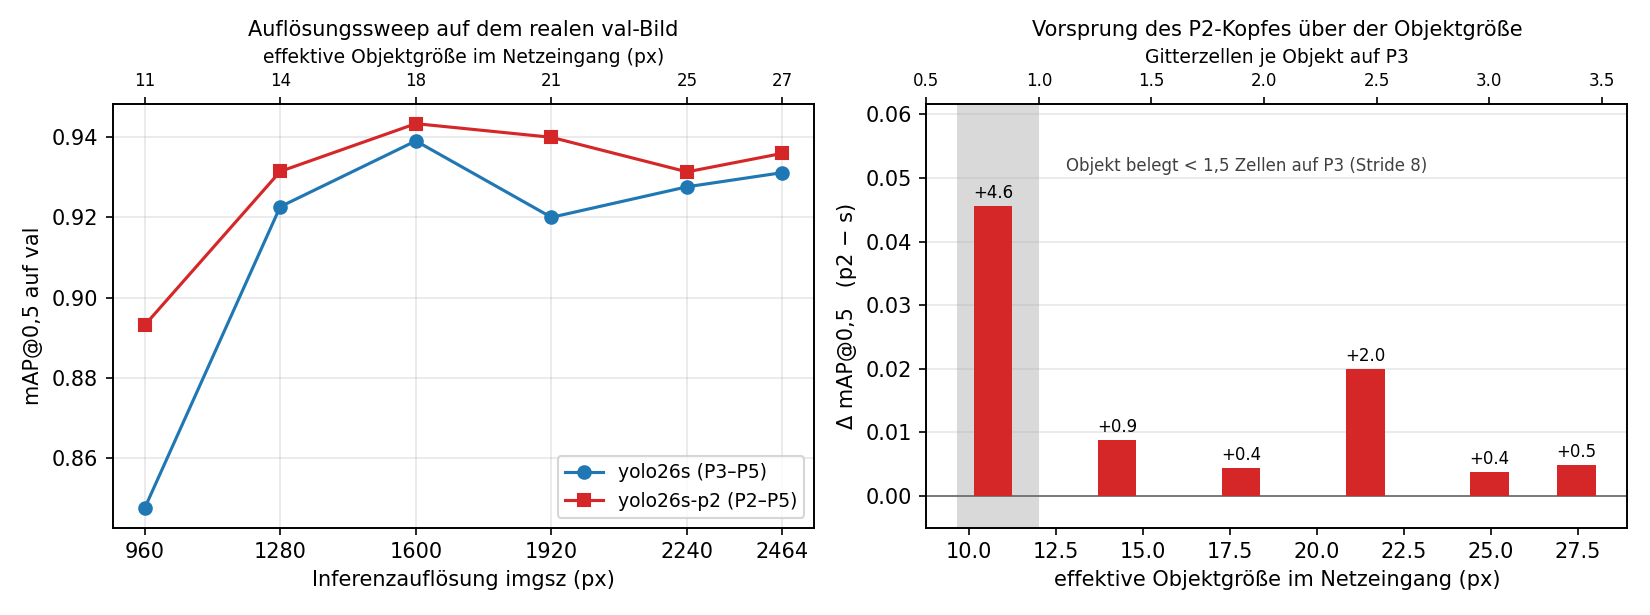
\includegraphics[width=\textwidth]{abbildungen/p2_sweep.png}
\caption[P2-Vorteil über der Auflösung]{Links: \mAPfifty{} auf dem realen
\code{val}-Bild über der Inferenzauflösung für beide Varianten; die obere Achse
nennt die zugehörige effektive Objektgröße im Netzeingang nach
Gleichung~\eqref{eq:deff}. Rechts: die Differenz beider Kurven. Der schattierte
Bereich markiert Objektgrößen unter $1{,}5$ Zellen auf P3, also den Bereich, in
dem die Rechnung aus Tabelle~\ref{tab:p2zellen} den größten Vorteil vorhersagt.}
\label{abb:p2sweep}
\end{figure}

Der Befund entspricht der Vorhersage: Bei \code{imgsz}=960 -- die Objekte
erreichen das Netz dann mit 10,7\px, also 1,3 Zellen auf P3 -- beträgt der
Vorsprung \textbf{4,6\PP}. Er ist damit rund zehnmal so groß wie bei den
Auflösungen, bei denen die Objekte über zwei Zellen belegen (0,4--0,9\PP{} bei
1600 und 1280). Anders formuliert: Der P2-Kopf leistet dasselbe wie eine
Verdopplung der Inferenzauflösung, solange die Objekte klein sind -- und wird
überflüssig, sobald sie groß genug sind. Das ist praktisch verwertbar: Wer die
Aufnahmeauflösung nicht frei wählen kann oder aus Laufzeitgründen bei kleiner
\code{imgsz} inferieren muss, gewinnt durch den P2-Kopf deutlich; wer ohnehin
hochskaliert, kaum. Der Punkt bei \code{imgsz}=1920 fällt mit $+2{,}0$\PP{} aus
diesem Muster; er verletzt die Monotonie und ist -- wie alle Differenzen dieser
Abbildung außer der bei 960 -- vom Konfidenzintervall
(Abschnitt~\ref{sec:bootstrap}) nicht zu unterscheiden.

\subsection{\mAPfifty{} und Zählfehler ordnen die Modelle gegenläufig}
\label{sec:p2zaehlung}

Der Vorteil des feineren Kopfes setzt sich \emph{nicht} in die Zielgröße der
Anwendung um. Am $F_1$-optimalen Betriebspunkt zählt \code{yolo26s-p2} auf
\code{test} 79 statt 86 Objekte -- ein Zählfehler von 8,1\,\% gegenüber 3,5\,\%
bei \code{yolo26s}, das dieselbe Aufnahme mit dem \emph{schlechteren}
\mAPfifty{} auswertet (0,905 gegen 0,941). Die Rangfolge kippt also, je nachdem
welche Größe man ansetzt.

Die Ursache ist die Schwellenwahl, nicht die Architektur: Das $F_1$-Optimum von
\code{yolo26s-p2} liegt bei $c^* = 0{,}379$ gegenüber $0{,}134$ und tauscht damit
Rückruf gegen Precision. Formal ist der Grund, dass $F_1$ beide Fehlerarten
\emph{gleich} gewichtet, der Zählfehler sich aber aus ihrer \emph{Differenz}
ergibt: Falsch-Positive und Falsch-Negative kompensieren sich in der Zählung
teilweise, im $F_1$ nie. Die beiden Optima müssen deshalb nicht zusammenfallen,
und hier tun sie es nicht.

Daraus folgt die praktisch wichtigste Aussage dieses Experiments: \textbf{Für
eine Zählanwendung ist mAP das falsche Auswahlkriterium, und der Betriebspunkt
wirkt stärker als die Architektur.} Der Betriebspunkt wäre direkt auf den
Zählfehler zu optimieren -- das wurde hier bewusst nicht getan, weil eine auf
\code{val} kalibrierte Zählschwelle die Aussagekraft der \code{test}-Zahlen
geschwächt hätte. Zu beachten ist der Umfang: Der Unterschied beruht auf
\emph{einem} Testbild mit 86 Objekten an je einem Betriebspunkt. Belastbar ist
der große Abstand von vier Objekten mit identifizierter Ursache, nicht eine
Rangfolge auf ein Objekt Genauigkeit.

\subsection{Einschränkungen und Konsequenz}

Drei Vorbehalte sind zu nennen. Erstens beruht der Vergleich auf \emph{je einem}
Trainingslauf pro Variante; die Streuung über Seeds ist unbekannt. Zweitens
liegen alle Differenzen außer der bei \code{imgsz}=960 innerhalb des
Bootstrap-Intervalls. Drittens ist der Vorteil bei \mAPall{} \emph{nicht}
konsistent: Über den Sweep hinweg ist \code{yolo26s-p2} bei drei von sechs
Auflösungen schlechter, was zur unveränderten Treffer-IoU passt -- P2 verbessert
das Finden, nicht das Lokalisieren.

Die Konsequenz für die Arbeit: Der P2-Kopf ist die wirksamste
\emph{architektonische} Maßnahme gegen das in
Abschnitt~\ref{sec:ioukleinobjekt} beschriebene Auflösungsproblem, und er ist
gegenüber der Alternative -- höhere Inferenzauflösung -- die
speichergünstigere Lösung, solange man die Trainingskosten einmalig aufbringen
kann. Für einen produktiven Einsatz wäre \code{yolo26s-p2} zu wählen; die in
dieser Arbeit dokumentierten Experimente~1 und~2 wurden auf der yolo11s-Baseline
gerechnet und bleiben davon unberührt, weil alle drei Modelle auf P3/P4/P5
dieselben Schrittweiten haben.

\section{Statistische Belastbarkeit und Fehleranalyse}
\label{sec:bootstrap}

Da je Split nur \emph{ein} Bild vorliegt, ist ein gewöhnlicher Bootstrap über
Bilder nicht möglich. Verwendet wird ein räumlicher Block-Bootstrap: Das Bild wird
in Kacheln zerlegt, über die mit Zurücklegen neu gezogen wird (400
Wiederholungen); die Blockbildung ist nötig, weil benachbarte Objekte nicht
unabhängig sind -- sie teilen Beleuchtung, Schärfe und Verdeckungssituation
\parencite{kuensch1989,efron1993}. Für \mAPfifty{} ergibt sich \code{val}
$0{,}892 \pm 0{,}051$ mit 95\,\%-Intervall $[0{,}766;\,0{,}965]$ (23 Kacheln) und
\code{test} $0{,}911 \pm 0{,}036$ mit $[0{,}844;\,0{,}974]$ (25 Kacheln). Alle in
diesem Kapitel berichteten Unterschiede unterhalb dieser Größenordnung sind als
Hinweis und nicht als Nachweis zu lesen; nicht betroffen ist der
Auflösungseffekt, dessen Größe von 47\PP{} das Intervall um ein Vielfaches
übersteigt.

\absatz{Falsch-Negative.} Sie treten fast ausschließlich bei sehr kleinen
Objekten am linken Bildrand von \code{test} (12--15\px), bei stark verdeckten
Enden tief im Stapel -- also dort, wo die Pipeline auch selbst kein Label mehr
vergäbe -- und bei Enden ohne sichtbaren hellen Kranz auf. Letzteres ist der
Fehlertyp, der auf die verbleibende Domänenlücke zurückgeht: Alle vier Clean
Plates sind bei diffusem Licht aufgenommen.

\absatz{Falsch-Positive.} Ihre Ursache unterscheidet sich zwischen den beiden
Bildern, und die Unterscheidung ist nicht kosmetisch. Auf \code{val} haben 9 der
11 Falsch-Positiven \emph{keinerlei} Überlappung mit einer Ground-Truth-Box; ein
Teil von ihnen sitzt auf erkennbaren Rohröffnungen, die in der Annotation fehlen.
Bei 88 handannotierten Objekten schlägt jede fehlende Annotation mit etwa
1,1\PP{} Precision zu Buche, die berichteten Precision-Werte sind also eine
\textbf{Untergrenze}. Die übrigen entstehen an dunklen Löchern im Maschendraht
und an Schattenspalten zwischen Rohren -- genau die Strukturen, gegen die die
Negativbilder gerichtet sind; dass sie dort noch auftreten, spricht dafür, dass
deren Anteil von 9,7\,\% eher an der Untergrenze des Sinnvollen liegt. Auf
\code{test} liegt der Fall völlig anders, und er ist Gegenstand des folgenden
Abschnitts.

\section{Ein systematischer Größenversatz der Boxen}
\label{sec:boxversatz}

Im Qualitativbild des Testbildes (Abbildung~\ref{abb:qualitativ} im Anhang)
liegen an mehreren Stellen eine rote und eine blaue Box nahezu deckungsgleich --
dieselbe Stirnfläche wird also gleichzeitig als Falsch-Positiv \emph{und} als
Falsch-Negativ gezählt. Das ist kein Darstellungsfehler, sondern die unmittelbare
Folge der Zuordnungsregel: Eine Detektion gilt nur als Treffer, wenn ihre IoU mit
der Ground-Truth-Box mindestens 0,5 beträgt. Liegt sie darunter, bleibt die
Detektion unzugeordnet (rot) und die Ground-Truth-Box unbedient (blau) -- ein und
dasselbe Objekt erzeugt zwei Fehler.

Auf \code{test} betrifft das \textbf{sechs der acht Falsch-Positiven}. Ihre IoU
liegt zwischen 0,401 und 0,497, in zwei Fällen wird die Schwelle um weniger als
0,005 verfehlt; alle sechs sitzen mit Konfidenzen zwischen 0,52 und 0,84 auf
annotierten Objekten. Senkt man allein die Zuordnungsschwelle von 0,50 auf 0,40,
so ergeben sich 81 Treffer, 2 Falsch-Positive und 5 Falsch-Negative statt
75/8/11 -- Abbildung~\ref{abb:qualitativ} im Anhang zeigt beide Fassungen
desselben Bildes mit identischer Detektionsmenge. Auf \code{val} tritt der
Effekt nicht auf; dort ändert dieselbe Absenkung nichts.

Die naheliegende Frage, ob damit nicht schon alles behoben sei, ist zu
verneinen. Eine niedrigere Schwelle verschiebt die \emph{Messkonvention}, nicht
die Ursache: Sie erklärt sechs Fehler weg, ohne dass die Boxen genauer würden,
und 0,50 ist der Bezugswert von PASCAL VOC und COCO
\parencite{everingham2010,lin2014coco}. Ein berichteter Wert bei 0,40 wäre nicht
mehr mit Literaturzahlen vergleichbar und stünde im Verdacht, die Metrik dem
Ergebnis angepasst zu haben. Die abgesenkte Schwelle ist deshalb ein
\emph{Diagnosewerkzeug} -- sie trennt Zuordnungsartefakte von echten Fehlern --,
und die Korrektur gehört an die Labelkonvention.

\absatz{Die Boxen sind systematisch zu klein.} Die Ursache lässt sich messen.
Tabelle~\ref{tab:boxversatz} vergleicht für jede Detektion, die eindeutig auf
einem annotierten Objekt sitzt ($\mathrm{IoU} > 0{,}3$), die vorhergesagte mit
der annotierten Boxgröße.

\begin{table}[htbp]
\centering
\caption[Größenversatz der Boxen]{Vergleich der vorhergesagten mit der
annotierten Boxgröße. Als Boxgröße dient $\sqrt{\text{Fläche}}$, der
Zentrumsversatz ist in Objektdurchmessern angegeben. \code{sval} ist der
synthetische Split, dessen Labels der Generator selbst erzeugt hat.}
\label{tab:boxversatz}
\footnotesize
\begin{tabular}{@{}lrrrrr@{}}
\toprule
\textbf{Split} & \textbf{Paare} & \textbf{Objekt-\Oe{} (Median)} &
\textbf{pred/GT} & \textbf{GT $-$ pred} & \textbf{Zentrumsversatz} \\
\midrule
\code{test} (real)        &   82 & 22,3\px & 0,884 & $+2{,}53$\px & 0,049\,\Oe \\
\code{val} (real)         &   75 & 27,5\px & 0,961 & $+1{,}16$\px & 0,054\,\Oe \\
\code{sval} (synthetisch) & 1064 & 22,0\px & \textbf{1,012} & $-0{,}29$\px & -- \\
\bottomrule
\end{tabular}
\end{table}

Der Befund ist eindeutig. Auf dem synthetischen Split trifft das Modell die
Boxgröße auf 1\,\% genau; auf den realen Bildern liegt sie 4\,\% (\code{val})
bzw.\ 12\,\% (\code{test}) darunter. Der Versatz ist dabei in \emph{absoluten}
Pixeln annähernd konstant und trifft deshalb die kleinsten Objekte am härtesten:
Bei Objekten unter 18\px{} beträgt das Verhältnis nur noch 0,830, bei über
26\px{} dagegen 0,894. Der Zentrumsversatz liegt mit rund 0,05
Objektdurchmessern (etwa 1\px) dagegen im Bereich der Annotationsgenauigkeit --
es handelt sich also um einen Größen-, nicht um einen Positionsfehler.

\begin{figure}[htbp]
\centering
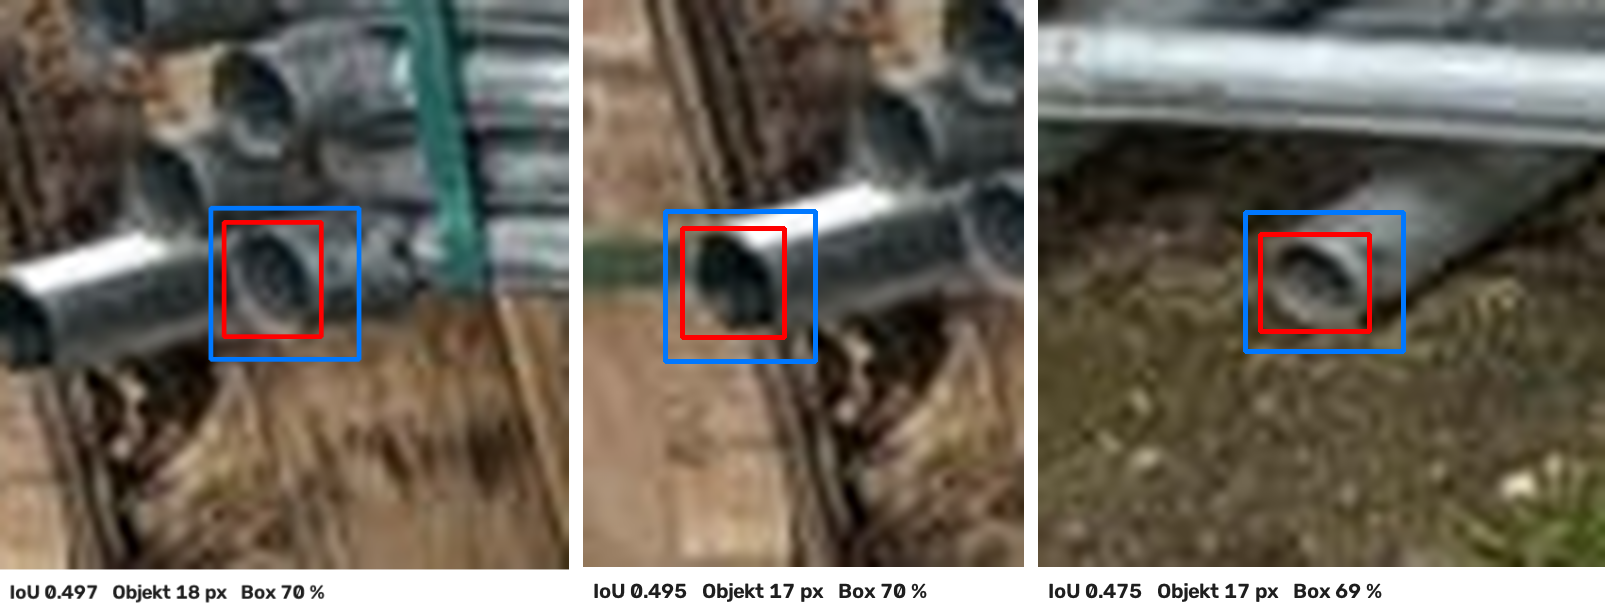
\includegraphics[width=\textwidth]{abbildungen/boxversatz.png}
\caption[Rote und blaue Box am selben Objekt]{Drei der sechs betroffenen Stellen
aus dem Testbild, neunfach vergrößert. Blau die Handannotation, rot die
Detektion. Alle drei Objekte sind gefunden, die vorhergesagte Box umfasst aber
nur etwa 70\,\% der annotierten Kantenlänge; die IoU bleibt damit knapp unter der
Zuordnungsschwelle 0,5, und dasselbe Objekt zählt als Falsch-Positiv \emph{und}
als Falsch-Negativ.}
\label{abb:boxversatz}
\end{figure}

\absatz{Modellfehler oder Labelkonvention?} Weil das Modell auf dem synthetischen
Split die Boxgröße nahezu exakt reproduziert, liegt die Ursache nicht in der
Boxregression, sondern in der \emph{Labelkonvention}: Die Generatorboxen folgen
der $\alpha > 0{,}5$-Kontur der Alphamaske
(Abschnitt~\ref{sec:sichtbarkeit}), die Handannotation umschließt das Objekt
großzügiger. Anforderung~A5 -- identische Labeldefinition in Quelle und Ziel --
ist damit nur \emph{annähernd} erfüllt; der Restversatz beträgt messbar 1,2 bis
2,5\px. Abbildung~\ref{abb:boxversatz} zeigt zugleich die Gegenprobe: Es sind die
kleinsten und kontrastärmsten Objekte, bei denen sich die Detektion auf die
dunkle Bohrung zusammenzieht, während die Annotation den hellen Kranz mit
einschließt. Ein Teil des Versatzes ist damit auch echte
Lokalisierungsschwierigkeit und nicht allein Konvention.

\absatz{Was der Versatz kostet.} Eine Sensitivitätsrechnung schätzt die
Größenordnung: Weitet man alle vorhergesagten Boxen um den gemessenen medianen
Fehlbetrag je Seite auf (1,27\px{} auf \code{test}, 0,58\px{} auf \code{val}) und
wertet neu aus, so ergibt sich Tabelle~\ref{tab:boxsens} im Anhang.

Auf \code{test} steigt \mAPseven{} von 0,320 auf 0,714 und \mAPall{} von 0,437
auf 0,604; auf \code{val}, wo der Versatz weniger als halb so groß ist, bewegt
sich entsprechend wenig. Damit ist auch der in
Abschnitt~\ref{sec:hauptergebnis} auffällige Unterschied zwischen den Splits
erklärt: Er geht nur zu einem Teil auf die kleinere Objektgröße in \code{test}
zurück, überwiegend aber auf die dort um 1,4\px{} großzügigere Annotation. Die
berichteten Werte für \mAPseven{} und \mAPall{} auf \code{test} sind folglich
\textbf{pessimistisch} -- sie messen zu einem erheblichen Teil eine
Konventionsdifferenz und nicht die Lokalisierungsgüte des Modells. Für
\mAPfifty{}, das $F_1$ und den Zählfehler -- die für die Anwendung maßgeblichen
Größen -- bleibt der Effekt klein.

\absatz{Konsequenz.} Die Korrektur ist einfach und sollte vor jeder weiteren
Optimierung erfolgen: Die Boxen des Generators sind an die Annotationskonvention
anzupassen, indem die Boxschwelle von $\alpha > 0{,}5$ herabgesetzt oder die
fertige Box um etwa 1\px{} je Seite aufgeweitet wird. Sauberer, aber teurer wäre
der umgekehrte Weg -- die 174 Handlabels nach derselben Regel neu zu ziehen, nach
der der Generator seine Boxen bildet. Solange beides nicht geschehen ist, sind
die Lokalisierungsmetriken dieser Arbeit untereinander vergleichbar, nicht aber
gegen Literaturwerte.

\chapter{Diskussion und Fazit}
\label{kap:diskussion}

\section{Was ist belegt, was ist nur begründet?}
\label{sec:tragend}

Kapitel~\ref{kap:pipeline} hat gezeigt, dass die Pipeline die Anforderungen
A1--A6 erfüllt. Das ist eine Aussage über den Entwurf, nicht über die Wirkung.
Für eine ehrliche Bilanz muss unterschieden werden zwischen Entscheidungen, deren
Nutzen \emph{gemessen} wurde, und Entscheidungen, die lediglich \emph{begründet}
sind:

\emph{Gemessen durch eigene Trainingsläufe} sind der Okklusionsanteil
(Abschnitt~\ref{sec:ablation}) und der P2-Detektionskopf
(Abschnitt~\ref{sec:p2}) -- in beiden Fällen liegt der Effekt jedoch weitgehend
innerhalb des Konfidenzintervalls, belastbar ist die Konsistenz, nicht die
Einzeldifferenz. \emph{Gemessen ohne Neutraining} sind Inferenzauflösung,
NMS-Schwelle, \code{max\_det} und Test-Time-Augmentation; nur der
Auflösungseffekt übersteigt das Konfidenzintervall deutlich. \emph{Kalibriert an
der erzeugten Verteilung} sind Objektgrößenbereich, Ovalisierungsanteil,
Gitterabstände, eine Basisgröße pro Cluster, Tiefenmodell 75/25 und Randregel --
hier trifft die erzeugte Statistik die reale (Tabelle~\ref{tab:kalibrierung}),
ohne dass der Nutzen für die Detektionsgüte separat gemessen wurde.
\emph{Indirekt gestützt} ist das Bündel der Anti-Abkürzungs-Maßnahmen S1--S6: Der
Sim-to-Real-Abstand von 9,6\PP{} ist -- statt eines Vielfachen, wie bei einer
durchlässigen Signatur zu erwarten -- ein Indiz, aber kein Nachweis für einzelne
Maßnahmen. \emph{Begründet, aber nicht belegt} bleiben Matting-Schwelle, Farb-,
Unschärfe- und Rauschangleich, JPEG-Requantisierung, Schlagschatten, Gamma, HSV,
Mulde, globale Bildstufe, Negativbildanteil sowie die Dellen- und
Perspektivanteile.

Von den 36 dokumentierten Transformationen ist damit der Trainingsnutzen von
dreien durch eine Ablation gemessen, sechs weitere sind an einer Realmessung
kalibriert, und die übrigen 27 sind begründet, aber nicht einzeln belegt.

\absatz{Die unbequeme Bilanz.} Der größte gemessene Einzeleffekt ist \emph{keine}
Augmentierungsentscheidung, sondern die Inferenzauflösung: 47\PP{} \mAPfifty{}
zwischen \code{imgsz}~640 und 1600. Alle Augmentierungsentscheidungen zusammen
bewegen sich in der Größenordnung weniger Prozentpunkte. Das relativiert den
Aufwand der Pipeline nicht -- ohne sie gäbe es überhaupt keinen
Trainingsdatensatz --, verschiebt aber die Priorität: Wer eine solche Anwendung
baut, sollte die Auflösungsfrage \emph{zuerst} klären und erst danach die
Feinheiten der Synthese optimieren.

\absatz{Was die beiden Experimente nicht beantworten.} Die Okklusionsablation
zeigt, \emph{dass} mehr Verdeckung hilft, aber nicht, ob deren
\emph{physikalische Plausibilität} nötig ist -- ein Arm mit gleich starker, aber
generischer Verdeckung (etwa Cutout) hätte das entschieden und fehlt. Damit
bleibt die aufwendigste Begründung der Pipeline, echte Rohrschäfte statt gemalter
Balken, unbelegt. Und der P2-Vergleich beruht auf je einem Trainingslauf pro
Variante, sodass die Streuung über Seeds unbekannt bleibt.

\section{Grenzen und nächste Schritte}
\label{sec:grenzen}

\absatz{Grenzen der Pipeline.} \emph{(1)} Nur neun Quellobjekte -- jedes
erscheint rund 15\,100-mal als gelabeltes Objekt. Die photometrische und
geometrische Streuung mildert das, hebt es aber nicht auf; Augmentierung erzeugt
keine neue Information über die Objektklasse. Das ist der Hauptgrund für die
Wahl eines kleinen Modells und der plausibelste Grund dafür, dass 6000 Bilder
gegenüber 3000 keinen Vorteil brachten. \emph{(2)} Nur diffuses Licht im
Quellmaterial: Harte Schlagschatten, Gegenlicht, Nässe und Schnee fehlen
vollständig und werden nur approximativ über die globale photometrische Stufe
angenähert -- die größte verbleibende Domänenlücke, von der Fehleranalyse
bestätigt. \emph{(3)} Reflect-Padding erzeugt Spiegelsymmetrie, wenn ein
Hintergrund für den gewünschten Zoom zu klein ist; eine spiegelsymmetrische
Bildhälfte ist selbst ein erkennbares Merkmal, die Maßnahme gegen Signatur~S1
erzeugt damit eine schwächere neue Auffälligkeit. \emph{(4)} Sieben Werte sind
Annahmen (Dellen, Perspektive, Schlagschatten, vertikale Spiegelung, globale
Farbtemperatur, Bewegungsunschärfe und die Clustergröße des Layoutmodells). \emph{(5)} Die synthetischen Cluster sind
dichter als real -- bewusst als Robustheitsreserve belassen; die umgekehrte
Abweichung wäre gefährlich gewesen. \emph{(6)} Die Schaftrichtung ist an der
gemessenen Säulenrichtung des Clusters kalibriert, nicht an der Rohrrichtung des
Hintergrunds: Sie entsteht als Senkrechte zur Säulenrichtung mit einer Streuung
von $55^\circ$ bis $125^\circ$, während die vier Clean Plates ihre Rohre
zwischen $-1{,}6^\circ$ und $+6{,}6^\circ$ zur Waagerechten haben
(Struktur-Tensor, \code{src/occluders.py}). In 19,1\,\% der Cluster kreuzt der
Schaft die Hintergrundrohre deshalb unter mehr als $60^\circ$; betroffen sind
21,6\,\% aller erzeugten Bilder. Weil alle Rohre eines Stapels parallel liegen,
ist das dieselbe Unstimmigkeit, gegen die die enge Streuung von $\pm11^\circ$
\emph{innerhalb} eines Clusters gesetzt ist -- zwischen Cluster und Hintergrund
wird sie nicht erzwungen. Auch hier geht die Abweichung in Richtung mehr
Variation, ihr Nutzen ist aber nicht geprüft; ein Angleich wäre billig, weil die
dominante Hintergrundrichtung gemessen vorliegt.

\absatz{Grenzen der Bewertung.} Die schwerwiegendste methodische Schwäche liegt
nicht in der Pipeline, sondern in der Bewertung: \emph{je ein Bild} pro Split.
Daraus folgen breite Konfidenzintervalle ($\pm 0{,}04$ bis $\pm 0{,}05$
\mAPfifty{}), sodass Unterschiede unterhalb dieser Größe nicht entscheidbar sind;
beide Bilder zeigen dieselbe Objektart bei ähnlichem Wetter, die Ergebnisse sagen
also nichts über andere Zaunhersteller, Rohrdurchmesser oder Lichtsituationen;
und die Ground Truth selbst ist unvollständig, weshalb die Precision-Werte eine
Untergrenze sind. Hinzu kommt der in Abschnitt~\ref{sec:boxversatz} gemessene
Größenversatz zwischen Generatorlabel und Handannotation von 1,2 bis 2,5\px:
Er macht \mAPseven{} und \mAPall{} auf \code{test} zu einem erheblichen Teil zu
einem Maß für die Labelkonvention statt für die Lokalisierungsgüte -- eine
Sensitivitätsrechnung hebt \mAPseven{} von 0,320 auf 0,714. Hinzu kommt, dass \code{val} doppelt verwendet wird -- für die
Modellauswahl \emph{und} für die Wahl der Inferenzauflösung. \code{test} ist
damit ein sauberer Endtest, \code{val} aber kein unabhängiger Bewertungssplit
mehr; die belastbaren Zahlen sind die \code{test}-Zahlen.

\absatz{Nächste Schritte.} Jede der genannten Grenzen hat eine Gegenmaßnahme;
nach erwartetem Nutzen geordnet: \emph{(0)} \textbf{Labelkonvention angleichen.}
Eine geänderte Boxschwelle im Generator genügt, und die Sensitivitätsrechnung
lässt auf \code{test} rund 39 Punkte \mAPseven{} erwarten -- der billigste große
Gewinn der Liste, zu erledigen vor jeder weiteren Optimierung.
\emph{(1)} \textbf{Mehr Bewertungsdaten.} Zehn
bis zwanzig annotierte Realbilder würden die Konfidenzintervalle auf ein Maß
bringen, bei dem beide Experimente entscheidbar wären -- mit Abstand der
wirksamste nächste Schritt. \emph{(2)}
\textbf{Leave-one-out-Ablation der Anti-Abkürzungs-Maßnahmen.} Je ein Lauf mit
abgeschaltetem Farb-, Rausch- und Unschärfeangleich sowie ohne JPEG-Durchlauf
würde erstmals belegen, welche Signatur tatsächlich ausgenutzt würde; Zielgröße
wäre der Sim-to-Real-Abstand, denn eine durchlässige Signatur müsste \code{sval}
nach oben und die realen Splits nach unten bewegen. \emph{(3)} \textbf{Ergänzende
Kontrollarme} -- eine labelzahl-kontrollierte Okklusionsablation mit einem
zusätzlichen Arm für generische statt physikalischer Verdeckung, und der direkte
Vergleich von P2-Kopf und kachelweiser Inferenz \parencite{akyon2022sahi} bei
gleichem Speicherbudget. \emph{(4)} \textbf{Breiteres Quellmaterial} -- zusätzliche
Clean Plates bei harter Sonne, Gegenlicht und Nässe gegen die Lücke aus
Punkt~\emph{(2)} der Pipelinegrenzen; die über 150 weiteren Objektausschnitte,
die aus den vorhandenen Realbildern zu gewinnen wären, stehen dagegen im
Zielkonflikt mit Punkt~\emph{(1)} dieser Liste.

\section{Fazit}

Ein ausschließlich auf synthetischen Bildern trainierter Detektor zählt auf zwei
echten, nie im Training gesehenen Aufnahmen mit einem \textbf{Fehler von
2,3\,\%} -- 86 statt 88 und 84 statt 86 Objekte. Für eine Anwendung, für die kein
einziges handannotiertes Trainingsbild existiert, ist das ein brauchbares
Ergebnis. Die zugehörigen Detektionsgüten sind \mAPfifty{} 0,886 und 0,888, bei
geeigneter Inferenzauflösung 0,928 und mit einem feineren Detektionskopf 0,947 --
letzterer allerdings bei \emph{schlechterem} Zählfehler
(Abschnitt~\ref{sec:p2zaehlung}).

Methodisch tragen fünf Einsichten:

\begin{enumerate}[itemsep=2pt]
  \item \textbf{Bei rein synthetischen Trainingsdaten ist die Pipeline die
  Hypothese.} Jede Entscheidung über eine Transformation ist eine Aussage
  darüber, welche Invarianzen in der Zieldomäne gelten. Die Begründungspflicht --
  Messung, physikalische Randbedingung oder ausgewiesene Annahme -- ist deshalb
  keine Formalität, sondern das eigentliche Handwerk.
  \item \textbf{Die dominante Fehlerquelle sind systematische Versätze, nicht
  fehlende Variation.} Farb-, Schärfe-, Rausch- und Kompressionsversatz zwischen
  eingefügten und originalen Pixeln lassen sich nicht durch mehr Zufall beheben;
  sie müssen einzeln geschlossen werden. Der gemessene Sim-to-Real-Abstand von
  9,6\PP{} -- klein genug zum Funktionieren, groß genug als Beleg gegen reines
  Artefaktlernen -- ist das beste verfügbare Indiz, dass dies gelungen ist.
  \item \textbf{Verdeckung ist bei dicht gepackten Kleinobjekten kein Beiwerk.}
  Stärkere physikalisch plausible Verdeckung verbessert das Ergebnis monoton --
  und zwar gegen einen Verlust von einem Drittel der Labels.
  \item \textbf{Auflösung ist die dominierende Größe, auf drei Ebenen:}
  Objektgrößenbereich des Generators, Inferenzauflösung (Faktor zwei in der
  Detektionsgüte) und Wahl des Detektionskopfes. Die Rechnung
  $\mathbb{E}[N_{\text{Zellen}}] = \pi d^2/(4S^2)$ verbindet alle drei -- sie sagt
  vorher, dass ein zusätzlicher Kopf auf Schrittweite~4 genau dort wirkt, wo die
  Objekte kleiner als etwa zwei Gitterzellen sind, und die Messung bestätigt das
  mit 4,6 gegenüber 0,4\PP{} Vorsprung.
  \item \textbf{Die Labelkonvention ist Teil des Messinstruments.} Ein
  systematischer Größenversatz von zwei Pixeln zwischen Generatorlabel und
  Handannotation kostet auf dem Testbild 39 Punkte \mAPseven{} -- mehr als jede
  Augmentierungsentscheidung einbringt. Wer Lokalisierungsmetriken bei
  20\px-Objekten berichtet, muss die Konvention beider Seiten zuerst
  gegeneinander prüfen.
\end{enumerate}


% ------------------------------- Verzeichnisse ----------------------------
\printbibliography[heading=bibintoc,title={Literaturverzeichnis}]

\appendix
\chapter{Anhang}
\label{kap:anhang}

\section{Reproduktion}

\begin{footnotesize}
\begin{verbatim}
# 0  Sichtung (erzeugt alle Messwerte aus Kapitel 4)
python src/analyze_data.py
# 1  Objektausschnitte freistellen  -> assets/masks/
python src/matting.py
# 2  Okkluder-Bibliothek            -> assets/bars/
python src/occluders.py
# 3  Trainingsdaten                 -> synth/train/ + generation_report.json
python src/generate.py --out synth/train --n 6000 --seed 1 --preview 8
python src/generate.py --out synth/sval  --n  400 --seed 99
# 4  Training
python src/train.py --name baseline
# 5  Auswertung (eigene Metriken + Kreuzvergleich)
python src/evaluate.py --weights runs/baseline/weights/best.pt \
    --splits val,test --crosscheck --out docs/experiments/final_eval.json
# 6  Experimente
python src/experiment.py infer          # Experiment 1 (Abschnitt 7.4)
python src/experiment.py ablation-data  # Experiment 2 (Abschnitt 7.5)
python src/experiment.py ablation-train
python src/experiment.py ablation-eval
python src/train.py --name yolo26s    --model yolo26s.pt
python src/train.py --name yolo26s_p2 --model yolo26s-p2.yaml \
    --pretrained yolo26s.pt
python src/experiment.py models         # Experiment 3 (Abschnitt 7.6)
# 7  Diagramme und Tabellen
python src/report.py
python paper/tools/fig_p2.py
python paper/tools/fig_boxversatz.py
python paper/tools/fig_qual_iou.py
python paper/tools/fig_stufen.py
python paper/tools/abbildungen_vorbereiten.py
\end{verbatim}
\end{footnotesize}

Eine Einschränkung der Ausführungsumgebung erzwingt einen Trainingsparameter: In
der verwendeten Kombination aus \code{opencv-python}~5.0.0.93 und
\code{torch}~2.13 verklemmt sich der fork-basierte DataLoader reproduzierbar beim
ersten Batch, sobald \code{workers > 0} gesetzt ist -- unabhängig von
\code{cv2.setNumThreads(0)}, deaktiviertem OpenCL, gesetzten Thread-Limits oder
der Startmethode \code{spawn}. Das Training läuft deshalb mit \code{workers=0}
und hält stattdessen alle dekodierten Bilder im Arbeitsspeicher
(\code{cache='ram'}, etwa 18\,GB); der Cache wird von einem Thread-Pool gefüllt
und ist vom Deadlock nicht betroffen.

\section{Gemessene Anteile aus dem Erzeugungsbericht}

Die folgenden Werte stammen unverändert aus
\code{synth/train/generation\_report.json} und sind die Belegquelle für alle
Ist-Anteile in Tabelle~\ref{tab:parameter}.

\begin{footnotesize}
\begin{verbatim}
n_images                      6000        instances_rendered      173100
canvas                        1024        instances_labeled       136384
boxes_per_image_mean          22.73       dropped_occluded         30801
mean_visibility_all_rendered   0.7569     dropped_offscreen         3846
mean_visibility_labeled        0.9002     dropped_tiny               228

inst_rotation      (je Instanz)  1.0000    negative_image  (je Bild)  0.0973
inst_oval          (je Instanz)  0.5707    img_has_bars    (je Bild)  0.5835
inst_dent          (je Instanz)  0.1814    img_clutter     (je Bild)  0.3157
inst_perspective   (je Instanz)  0.3020    recess          (je Bild)  0.8738
inst_photometric   (je Instanz)  0.9976    bg_fliplr       (je Bild)  0.5047
inst_gamma         (je Instanz)  0.7969    bg_flipud       (je Bild)  0.1487
inst_hsv           (je Instanz)  0.6973    bg_rot          (je Bild)  0.3428
inst_harmonize     (je Instanz)  0.8482    glob_bc         (je Bild)  0.8958
inst_blur          (je Instanz)  0.5983    glob_hsv        (je Bild)  0.6897
inst_noise         (je Instanz)  0.6988    glob_blur       (je Bild)  0.3435
inst_shadow        (je Instanz)  0.4931    glob_motion     (je Bild)  0.0988
inst_stub          (je Instanz)  0.8801    glob_noise      (je Bild)  0.8015
inst_occluded (je Label)         0.3009    glob_vignette   (je Bild)  0.2502
\end{verbatim}
\end{footnotesize}

Ein Wert ist nicht als Anteil lesbar: \code{recess} zählt die \emph{Anzahl} der
abgedunkelten Mulden je Bild. Der Sollwert ist 0,55 je Cluster, die erwartete
Clusterzahl beträgt
$0{,}45 \cdot 1 + 0{,}35 \cdot 2 + 0{,}20 \cdot 3 = 1{,}75$, und unter
Berücksichtigung der 9,7\,\% Negativbilder ergibt sich
$0{,}55 \cdot 1{,}75 \cdot 0{,}903 = 0{,}869$ -- was den gemessenen Wert 0,8738
erklärt. \code{img\_has\_bars} ist dagegen ein echter Anteil; der Sollwert 0,65
reduziert sich durch die Negativbilder auf $0{,}65 \cdot 0{,}903 = 0{,}587$ und
trifft den gemessenen Wert 0,5835.

\section{Vollständiger Sweep der Inferenzauflösung}

Tabelle~\ref{tab:imgszvoll} ergänzt den Auszug aus
Abschnitt~\ref{sec:imgsz} um die fehlenden Stufen.

\begin{table}[htbp]
\centering
\caption[Vollständiger Auflösungssweep]{Vollständiger Sweep der
Inferenzauflösung für die yolo11s-Baseline.}
\label{tab:imgszvoll}
\footnotesize
\begin{tabular}{@{}lrrrrrr@{}}
\toprule
\code{imgsz} & \multicolumn{3}{c}{\code{val}} & \multicolumn{3}{c}{\code{test}} \\
 & \mAPfifty{} & \mAPall{} & $F_1$ & \mAPfifty{} & \mAPall{} & $F_1$ \\
\midrule
640  & 0,435 & 0,201 & 0,507 & 0,524 & 0,335 & 0,620 \\
800  & 0,793 & 0,428 & 0,768 & 0,665 & 0,363 & 0,699 \\
960  & 0,852 & 0,498 & 0,840 & 0,889 & 0,430 & 0,855 \\
1024 & 0,868 & 0,546 & 0,876 & 0,882 & 0,459 & 0,841 \\
1280 & 0,887 & 0,577 & 0,861 & 0,900 & 0,449 & 0,907 \\
1600 & 0,904 & 0,606 & 0,850 & 0,888 & 0,437 & 0,894 \\
1920 & 0,893 & 0,613 & 0,851 & 0,928 & 0,448 & 0,917 \\
2240 & 0,880 & 0,588 & 0,843 & 0,928 & 0,457 & 0,920 \\
2464 & 0,886 & 0,597 & 0,862 & 0,927 & 0,454 & 0,928 \\
\bottomrule
\end{tabular}
\end{table}

\section{Sensitivität gegenüber dem Größenversatz}

Die Rechnung zu Abschnitt~\ref{sec:boxversatz}: Alle vorhergesagten Boxen werden
um den gemessenen medianen Fehlbetrag je Seite aufgeweitet (1,27\px{} auf
\code{test}, 0,58\px{} auf \code{val}) und neu ausgewertet.

\begin{table}[htbp]
\centering
\caption[Sensitivität gegenüber dem Größenversatz]{Sensitivitätsrechnung: alle
vorhergesagten Boxen um den medianen Fehlbetrag je Seite aufgeweitet. Das ist
\emph{kein} Ergebnis eines neuen Trainings, sondern eine Obergrenzenschätzung für
den Effekt einer angeglichenen Labelkonvention.}
\label{tab:boxsens}
\footnotesize
\begin{tabular}{@{}llrrrrr@{}}
\toprule
\textbf{Split} & & \mAPfifty{} & \mAPseven{} & \mAPall{} &
\textbf{bestes $F_1$} & \textbf{mittl.\ IoU} \\
\midrule
\code{test} & unverändert       & 0,887 & 0,320 & 0,437 & 0,894 & 0,748 \\
\code{test} & Boxen aufgeweitet & \textbf{0,951} & \textbf{0,714} &
\textbf{0,604} & \textbf{0,959} & \textbf{0,805} \\
\addlinespace
\code{val}  & unverändert       & 0,886 & 0,793 & 0,597 & 0,862 & 0,824 \\
\code{val}  & Boxen aufgeweitet & 0,886 & 0,812 & 0,622 & 0,862 & 0,835 \\
\bottomrule
\end{tabular}
\end{table}

\section{Verfahrensklassen der Bildaugmentierung}

\begin{table}[htbp]
\centering
\caption[Verfahrensklassen der Bildaugmentierung]{Verfahrensklassen der
Bildaugmentierung und ihr Einsatz im vorliegenden Fall.}
\label{tab:taxonomie}
\footnotesize
\begin{tabularx}{\textwidth}{@{}L{0.19\textwidth}X@{}}
\toprule
\textbf{Klasse} & \textbf{Einsatz hier} \\
\midrule
geometrisch, bildweit \newline
\scriptsize\cite{krizhevsky2012}; \cite{simard2003} &
Spiegelung, Skalierung, Translation: ja. Rotation, Scherung und Perspektive
bildweit: nein -- Labelrauschen (Abschnitt~\ref{sec:boxrotation}) \\
\addlinespace
geometrisch, pro Instanz \newline
\scriptsize\cite{dwibedi2017}; \cite{ghiasi2021} &
ja, im Generator mit exakter Neuberechnung der Box aus der Alphamaske \\
\addlinespace
photometrisch \newline
\scriptsize\cite{krizhevsky2012}; \cite{grossberg2003} &
ja, zweistufig -- pro Instanz und global \\
\addlinespace
Degradation \newline
\scriptsize\cite{hendrycks2019} &
ja (Unschärfe, Rauschen, JPEG, Vignettierung); hier zusätzlich als Mittel gegen
Einfügeartefakte (Abschnitt~\ref{sec:shortcut}) \\
\addlinespace
Informationsentzug \newline
\scriptsize\cite{devries2017cutout}; \cite{zhong2020erasing};
\cite{singh2017hideseek} &
nicht in generischer Form; ersetzt durch physikalisch motivierte Verdeckung mit
berechneter Sichtbarkeit (Tabelle~\ref{tab:parameter}, T6) \\
\addlinespace
Mehrbild-Mischung \newline
\scriptsize\cite{zhang2018mixup}; \cite{yun2019cutmix}; \cite{bochkovskiy2020} &
nur Mosaic; mixup und CutMix aus \\
\addlinespace
Synthese \newline
\scriptsize\cite{dvornik2018}; \cite{tobin2017}; \cite{tremblay2018} &
ja -- Kern des Verfahrens (Abschnitt~\ref{sec:augsynthese}) \\
\bottomrule
\end{tabularx}
\end{table}

\section{Alle Transformationen der Synthese-Pipeline}

{\footnotesize
\begin{longtable}{@{}L{0.195\textwidth}L{0.065\textwidth}L{0.55\textwidth}L{0.022\textwidth}@{}}
\caption[Alle Transformationen der Pipeline]{Alle 36 Transformationen der
Pipeline mit Parameterbereich, gemessenem Ist-Anteil und Begründung. \emph{S}
verweist auf die geschlossene Abkürzung aus Abschnitt~\ref{sec:shortcut},
\emph{Art} auf die Belegart (M/P/L/A) wie in Tabelle~\ref{tab:befunde}.}
\label{tab:parameter}\\
\toprule
\textbf{Transformation} & \textbf{Ist} & \textbf{Begründung} & \textbf{Art} \\
\midrule
\endfirsthead
\multicolumn{4}{@{}l}{\itshape Fortsetzung von Tabelle~\ref{tab:parameter}}\\
\toprule
\textbf{Transformation} & \textbf{Ist} & \textbf{Begründung} & \textbf{Art} \\
\midrule
\endhead
\bottomrule
\endfoot
\multicolumn{4}{@{}l}{\textbf{T1 -- Hintergrund} \hfill\emph{Anteile je Bild}}\\
Clean Plate statt Fremdszene & 80\,\%$^\ast$ & Die vier Clean Plates sind exakt die Zieldomäne (sechsfaches Ziehgewicht); die Fremdszenen liefern Kontextvielfalt und harte Negative. & M \\
Zoom an Rohr-\Oe{} gekoppelt, Gl.~\eqref{eq:zoom} & 100\,\% & Eine Stirnfläche hat zwangsläufig den Durchmesser des Schafts daneben; ein Missverhältnis trainierte eine falsche Kontext-Größen-Relation an. & P \\
Zufallsausschnitt (Translation) & 100\,\% & Bei nur sieben Quellbildern die wichtigste Quelle von Hintergrundvielfalt. & L \\
Reflect-Padding, max.\ $1{,}35\times$ kürzeste Kante & bei Bedarf & Kachelung erzeugte harte achsparallele Nähte; gespiegeltes Padding hat keine Kante. & L \\
horizontale Spiegelung & 50,5\,\% & Label-exakt und physikalisch korrekt: Ein Stapel wird von beiden Enden fotografiert. & P \\
vertikale Spiegelung & 14,9\,\% & Ebenfalls label-exakt, bewusst seltener -- die Schwerkraft erzeugt eine schwache Vorzugsrichtung. & A \\
Kleinrotation $\pm6^\circ$ (Zoom 1,06) & 34,3\,\% & Die Rohrlinien sind nie exakt achsparallel; wirkt vor dem Einfügen, betrifft also keine Boxen. & M \\
\addlinespace
\multicolumn{4}{@{}l}{\textbf{T2 -- Instanzgeometrie} \hfill\emph{Anteile je gerenderter Instanz}}\\
Rotation $0$--$360^\circ$ & 100\,\% & Rohrenden haben keine kanonische Orientierung -- die einzige Orientierungsinformation ist das Glanzlicht, und dessen Richtung hängt vom Sonnenstand ab. Volle Rotationsinvarianz ist korrekt \emph{und} kostenlos, daher 100\,\% statt eines Bruchteils. & P \\
Skalierung auf 12--44\px, Gl.~\eqref{eq:oval} & 100\,\% & Realmessung 12,2--35,8\px{} plus 25\,\% Reserve; Ist-Verteilung p05/Median/p95 = 11,6/22,5/39,9\px. Verkleinerung flächentreu, weil bilineare Interpolation Aliasing im Objekt zurückließe. & M (S3) \\
Ovalisierung 0,66--0,97 bzw.\ 1,03--1,30 & 57,1\,\% & Gemessenes Seitenverhältnis p10--p90 = 0,85--1,31; über die Hälfte der echten Boxen weicht um $\geq5\,\%$ vom Quadrat ab. Oblat dominiert (45:12), weil Schrägansicht die Höhe verkürzt. & M \\
Delle, 1--2 Sektoren, Tiefe 10--30\,\% & 18,1\,\% & Mechanisch beschädigte Enden. \textbf{Anteil ist Annahme} -- Dellen sind nicht annotiert. 18\,\% lässt das Modell die Verformung regelmäßig sehen, ohne die Rundheit als Merkmal zu verwässern. & A \\
Perspektive, Homographie $\pm9\,\%$ & 30,2\,\% & Bei Schrägblick wird der Kranz einseitig \emph{breiter} (sichtbare Rohrinnenwand); anisotrope Skalierung kann das nicht abbilden. Anteil ist Annahme. & A \\
\addlinespace
\multicolumn{4}{@{}l}{\textbf{T3 -- Photometrie und Einbettungsrealismus} \hfill\emph{je Instanz}}\\
Helligkeit $\times0{,}70$--$1{,}35$ & 99,8\,\% & Stirnflächen liegen in praller Sonne oder tiefem Schatten; Spannweite aus den Ausschnitten ablesbar (Kranzhelligkeit 88--156 Grauwerte). & M \\
Gamma $0{,}75$--$1{,}35$ & 79,7\,\% & Gamma statt Kontrast, weil es die nichtlineare Tonwertkurve verschiedener Kameras abbildet \parencite{grossberg2003} und das Verhältnis Bohrung $\leftrightarrow$ Kranz verändert. & L \\
HSV: Ton $\pm8^\circ$, Sättigung $\times0{,}45$--$1{,}60$ & 69,7\,\% & Verzinkter Stahl ist neutralgrau, nimmt aber Farbstiche an (Flugrost, Moos, Himmelsreflex); Farbtonhub klein, da große Sprünge unphysikalisch wären. & M \\
Farbangleich an den lokalen Hintergrund, Gl.~\eqref{eq:harmonize} & 84,8\,\% & \textbf{Wichtigste Anti-Abkürzungs-Maßnahme:} Ohne Angleich bleibt ein konstanter Farb- und Helligkeitsversatz, den ein CNN trivial als Einfügemarke lernt. Bewusst nur partiell. & L (S2) \\
Unschärfeangleich $\sigma$ 0,25--1,10\px & 59,8\,\% & Das skalierte Objekt ist glatter oder schärfer als das Zielbild, und reale Objekte liegen je nach Stapeltiefe außerhalb der Schärfeebene \parencite{popescu2005}. & L (S3) \\
Rauschangleich, Gl.~\eqref{eq:noise} & 69,9\,\% & Beim Verkleinern sinkt das Rauschen, der eingeklebte Bereich wäre messbar sauberer. Niveau \emph{pro Einfügestelle} geschätzt (Hintergründe: 6,8--15,2 Grauwerte Hochpassstreuung). & L (S4) \\
Alphakante weichzeichnen $\sigma$ 0,4--1,0\px & 100\,\% & Immer -- eine pixelharte Silhouette gibt es bei 25\px-Objekten in echten Aufnahmen nicht. & P (S1) \\
Schlagschatten, $\kappa$ 0,18--0,45 & 49,3\,\% & Ohne Kontaktschatten \enquote{schwebt} ein eingeklebtes Objekt sichtbar; rund 50\,\%, weil bei diffusem Licht etwa die Hälfte der realen Objekte keinen sichtbaren Schatten wirft (Annahme). & A (S6) \\
\addlinespace
\multicolumn{4}{@{}l}{\textbf{T4 -- Layout}}\\
gescherte Gitterpackung, 1--3 Cluster, Gl.~\eqref{eq:layout} & 100\,\% & Kalibriert am gemessenen NN-Abstand und an der Nachbarzahl (Tabelle~\ref{tab:kalibrierung}); eine Basisgröße pro Cluster nach Befund~7. & M \\
\quad Gitterabstände $s_1$, $s_2$ & -- & $s_1 \in [0{,}98;\,1{,}60]\,d_0$ und $s_2 \in [0{,}98;\,1{,}85]\,d_0$. Untergrenze physikalisch: Rohrzentren liegen mindestens einen Durchmesser auseinander. Die Obergrenzen sind an Median und p90 des NN-Abstands eingestellt. & P/M \\
\quad Gitterrauschen $\sigma$ & -- & $\sigma = 0{,}17\,d_0$. Setzt p10 und Berührungsquote; ohne diesen Term entstünden sichtbar künstliche Reihen. & M \\
\quad Winkel zwischen $\mathbf{e}_1$ und $\mathbf{e}_2$: $55^\circ$--$125^\circ$ & 100\,\% & Scherung des Gitters, abgeleitet aus dem Histogramm der Nachbarrichtungen (quasi isotrop, Häufung $90$--$150^\circ$). & M \\
\quad Clustergröße $n_1 \le 13$, $n_2 \le 6$ & -- & Steuert Nachbarzahl und Objektzahl je Bild (erzeugt: 22,7 Objekte je Bild), ist aber nicht einzeln kalibriert -- die Realbilder geben keine Clusterausdehnung her (Annahme). & A \\
abgedunkelte Mulde je Cluster & 0,87 je Bild & Die Stirnflächen liegen vor dem verschatteten Stapelinneren; ohne Abdunklung stünden die dunklen Bohrungen kontrastmäßig zu isoliert da. & M \\
\addlinespace
\multicolumn{4}{@{}l}{\textbf{T5 -- Rohrschaft} \hfill\emph{je Instanz}}\\
echter Rohrschaft dahinter, Länge 2--24\,\Oe & 88,0\,\% & \textbf{Wichtigste Einzelentscheidung} (Befund~8): Ein dunkler Kreis mitten auf einem durchgehenden Rohr ist physikalisch unmöglich. Lange Schäfte, weil real jedes Rohr aus dem Ausschnitt herausläuft; kurze Stummel wären ein verräterisches Muster. & P \\
Schaftrichtung je Cluster parallel, $\pm11^\circ$ & 100\,\% & Alle Rohre eines Stapels liegen parallel; $\pm18^\circ$ erzeugte einen sternförmigen Fächer, den es real nicht gibt. Die Bedingung gilt \emph{innerhalb} eines Clusters; gegen die
Rohrrichtung des Hintergrunds ist sie nicht erzwungen
(Abschnitt~\ref{sec:grenzen}). & P \\
Helligkeitsangleich des Schafts, $\kappa$ 0,35--0,75 & 100\,\% & Die Bibliothek stammt aus vier Aufnahmen mit Hintergrundmittel 70--102 Grauwerten; ohne Angleich klebten sichtbar zu dunkle Rohre im Bild. & M \\
Tiefenmodell: 75\,\% ganz hinten, 25\,\% eingereiht & -- & An der erzeugten Statistik kalibriert: Mit zufälliger Tiefenordnung stieg der synthetische NN-Abstand auf $1{,}55\,\Oe$, rund 40\,\% über dem realen Wert; mit 75/25 liegt er bei $1{,}17\,\Oe$. & M \\
\addlinespace
\multicolumn{4}{@{}l}{\textbf{T6 -- Okklusion} \hfill\emph{Anteile je Bild}}\\
quer liegende echte Rohrstangen, 1--6 Stück & 58,4\,\% & Rohre vor dem Stapel, Breite $0{,}55$--$1{,}35\,\Oe$; zu 80\,\% durch ein Cluster gelegt statt ins Leere, weil eine Verdeckung ohne getroffenes Objekt keinen Trainingsnutzen hat. & M \\
Fremdkörper (Laub, Draht, Schnee), 1--4 Stück & 31,6\,\% & Aus den Hintergründen selbst geschnitten, mit weicher Maske aus geglättetem Rauschen -- gleiches Quellmaterial, also gleiche Sensorsignatur. & M \\
\addlinespace
\multicolumn{4}{@{}l}{\textbf{T8 -- Globale Bildstufe} \hfill\emph{Anteile je Bild}}\\
Helligkeit/Kontrast $\times0{,}80$--$1{,}22$, Offset $\pm18$ & 89,6\,\% & Wetter- und Belichtungsvariation. & M \\
HSV / Farbtemperatur & 69,0\,\% & Bewölkt bis Abendsonne; da alle Clean Plates bei diffusem Licht entstanden, ist diese Stufe der einzige -- approximative -- Ersatz für die fehlende Beleuchtungsvielfalt. & A \\
Defokus $\sigma$ 0,3--1,0\px & 34,4\,\% & Der Autofokus trifft bei Stapelaufnahmen oft die falsche Ebene. & L \\
Bewegungsunschärfe, Kern 3--8\px & 9,9\,\% & Verwacklung aus der Hand; niedriger Anteil, weil moderne Mobiltelefone kurz belichten (Annahme). & A \\
Sensorrauschen $\sigma$ 1,0--5,0 & 80,1\,\% & Vereinheitlicht das Rauschniveau über das ganze Bild. & L \\
Vignettierung 10--35\,\% & 25,0\,\% & Weitwinkelobjektive; erzwingt zusätzlich Positionsinvarianz der Helligkeit. & L \\
JPEG-Requantisierung $q \in [55, 95]$ & 85\,\%$^\ast$ & \textbf{Wichtigste unsichtbare Transformation:} Eingeklebte Pixel behalten sonst eine andere DCT-Blockstatistik als der bereits einmal komprimierte Hintergrund \parencite{wallace1992jpeg}; ein erneuter Durchlauf über das \emph{Gesamtbild} vereinheitlicht sie. Forensisch die belastbarste Einfügemarke \parencite{farid2009}. & L (S5) \\
\addlinespace
\multicolumn{4}{@{}l}{\textbf{T9 -- Negativbilder}}\\
Bilder ohne jedes Objekt & 9,7\,\% & Bestraft die dominanten Falschpositiv-Quellen (Rohrschäfte, Gitterknoten, Löcher im Maschendraht) direkt; statisches Gegenstück zum Hard-Example-Mining \parencite{shrivastava2016}. Rund 10\,\% entspricht der Empfehlung der Werkzeugkette \parencite{ultralyticsdocs}. & M/L \\
\addlinespace
\multicolumn{4}{@{}l}{\footnotesize $^\ast$ konfigurierter Sollwert; im Bericht nicht separat gezählt.}\\
\end{longtable}
}

\section{Augmentierungsparameter zur Trainingszeit}

\begin{table}[htbp]
\centering
\caption[Augmentierungsparameter zur Trainingszeit]{Augmentierungsparameter des
Trainings; Standardwerte der Werkzeugkette nach \textcite{ultralyticsdocs}.}
\label{tab:trainaug}
\footnotesize
\begin{tabularx}{\textwidth}{@{}L{0.155\textwidth}L{0.05\textwidth}X@{}}
\toprule
\textbf{Parameter} & \textbf{Wert} & \textbf{Begründung} \\
\midrule
\code{mosaic} & 1,0 &
Immer aktiv \parencite{bochkovskiy2020}: erhöht die Objektzahl pro Iteration,
bringt Objekte an Kachelränder (in \code{test} sind 5,8\,\% der Labels
angeschnitten) und kombiniert Hintergründe. Boxen bleiben exakt. \\
\code{close\_mosaic} & 10 &
Abschalten in den letzten zehn Epochen: Vierfachkacheln sind eine Bildstatistik,
die es zur Inferenzzeit nie gibt. \\
\code{scale} & 0,4 &
Skalierung $0{,}6$--$1{,}4$. Der Standardwert 0,5 wurde reduziert, weil er die
kleinsten Objekte auf 6\px{} schrumpfen lässt -- unter der Auflösung von
Stride~8 und damit reines Labelrauschen. \\
\code{translate} & 0,1 &
Standard; verhindert eine Positionsverzerrung zur Bildmitte. \\
\code{fliplr} & 0,5 &
Label-exakt und physikalisch korrekt. \\
\code{flipud} & 0,5 &
Ebenfalls label-exakt. Für Naturbilder unüblich, hier richtig: Ein Rohrende hat
kein \enquote{oben}. \\
\code{hsv\_h/s/v} & 0,015 / 0,7 / 0,4 &
Kleiner Farbtonversatz (verzinkter Stahl ist neutral), kräftige
Sättigungsvariation (neutralgrau bis rostbraun), Helligkeitsvariation für
Sonne und Schatten. \\
\midrule
\code{degrees} \code{shear} \code{perspective} & 0,0 &
\textbf{Bewusst aus.} Bildrotation bläht achsparallele Boxen auf -- bei
$10^\circ$ um 15,8\,\% der Kantenlänge, was die Überlappung mit der korrekten Box
auf 0,745 senkt (Abschnitt~\ref{sec:boxrotation}). Die nötige Rotations- und
Perspektivinvarianz liefert der Generator label-exakt. \\
\code{mixup} \code{cutmix} & 0,0 &
\textbf{Aus.} Beide überlagern Bildinhalte bei erhaltenen Labels
\parencite{zhang2018mixup,yun2019cutmix} und erzeugen damit Geisterobjekte mit
vollem Boxlabel; bei dicht gepackten 20\px-Objekten überwiegt der
Labelkonflikt. Verdeckung entsteht stattdessen im Generator physikalisch korrekt. \\
\code{erasing} & 0,0 &
\textbf{Aus.} Random Erasing \parencite{zhong2020erasing} wirkt in der
Werkzeugkette nur bei der Klassifikation; die Funktion übernimmt die
Okklusionsstufe des Generators. \\
\code{copy\_paste} & 0,0 &
\textbf{Aus} -- benötigt Segmentierungsmasken. Copy-Paste
\parencite{ghiasi2021} ist genau das, was der Generator offline und mit
korrekter Sichtbarkeitsrechnung leistet. \\
\bottomrule
\end{tabularx}
\end{table}


\section{Beispielbilder und Qualitativergebnis}

\begin{figure}[htbp]
\centering
\begin{subfigure}{0.245\textwidth}
  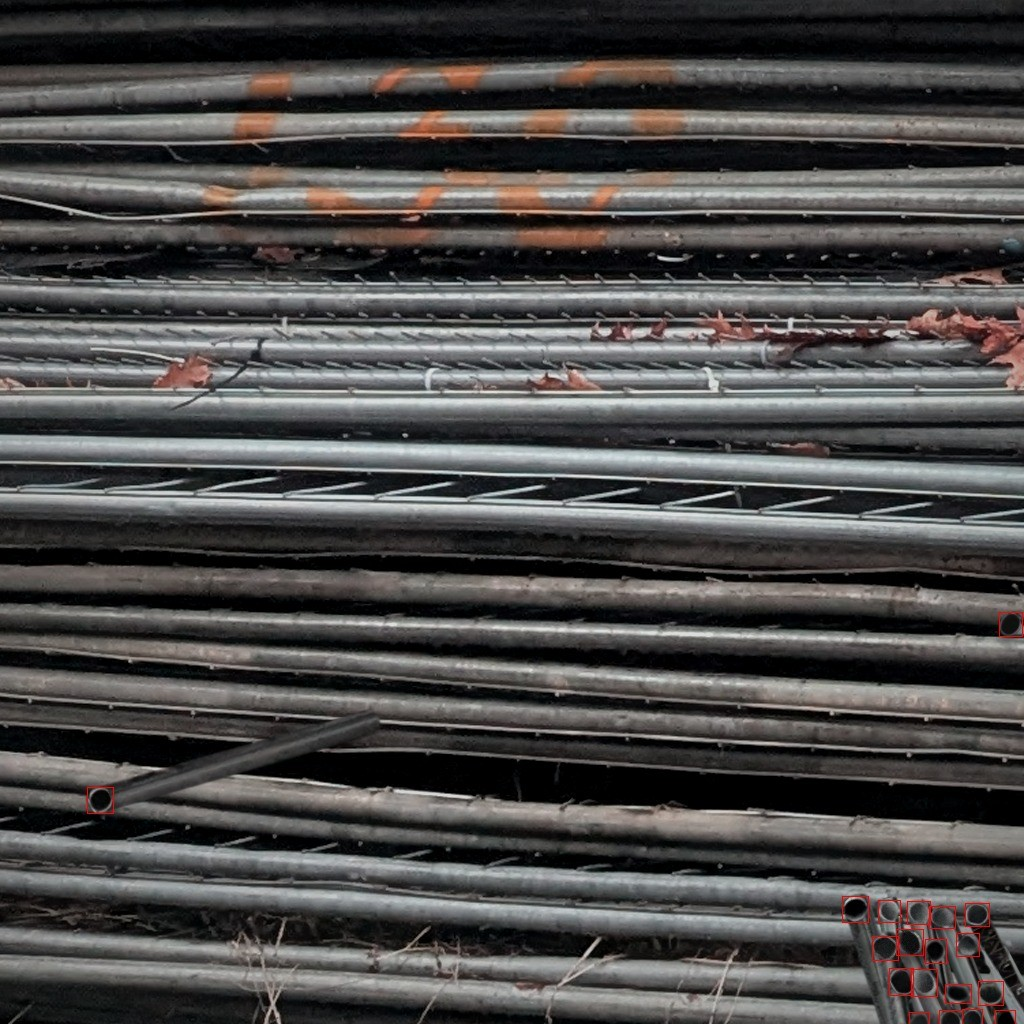
\includegraphics[width=\textwidth]{abbildungen/synth_000.jpg}
\end{subfigure}\hfill
\begin{subfigure}{0.245\textwidth}
  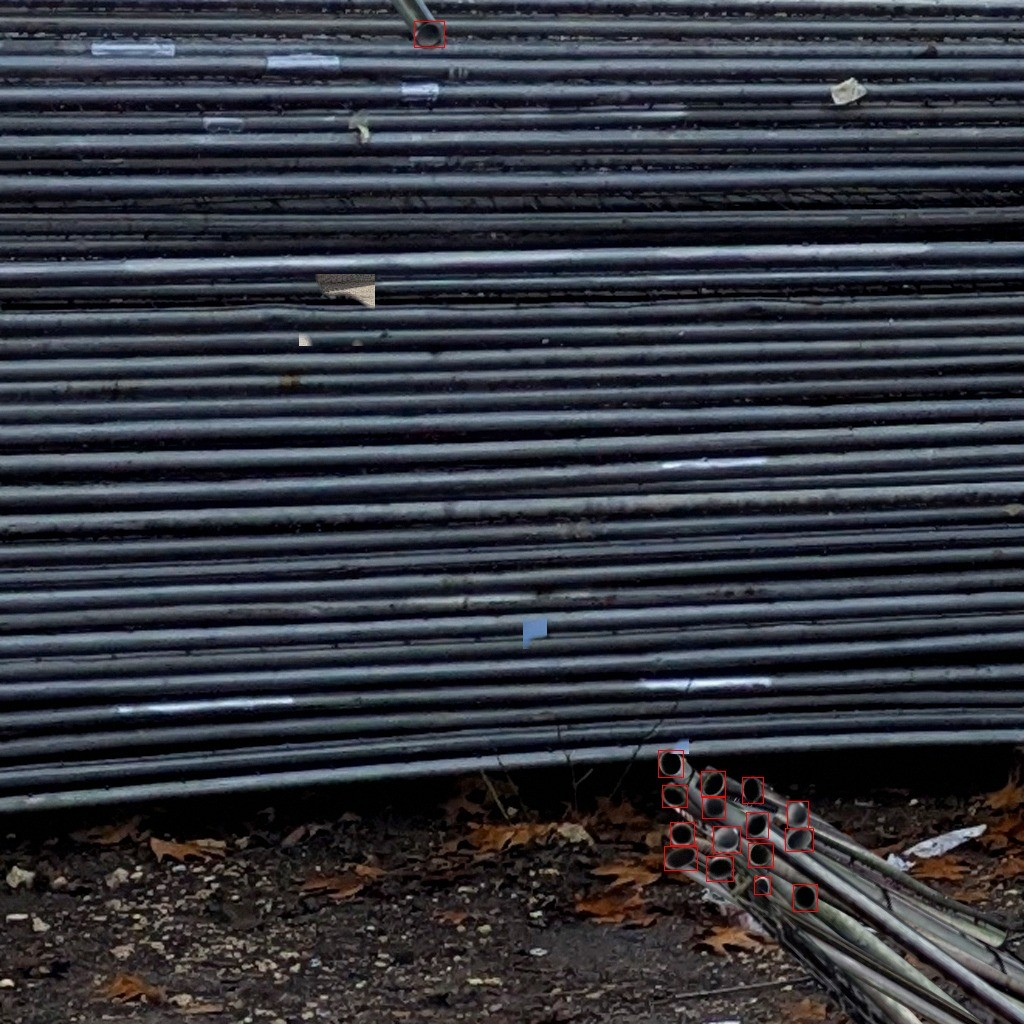
\includegraphics[width=\textwidth]{abbildungen/synth_001.jpg}
\end{subfigure}\hfill
\begin{subfigure}{0.245\textwidth}
  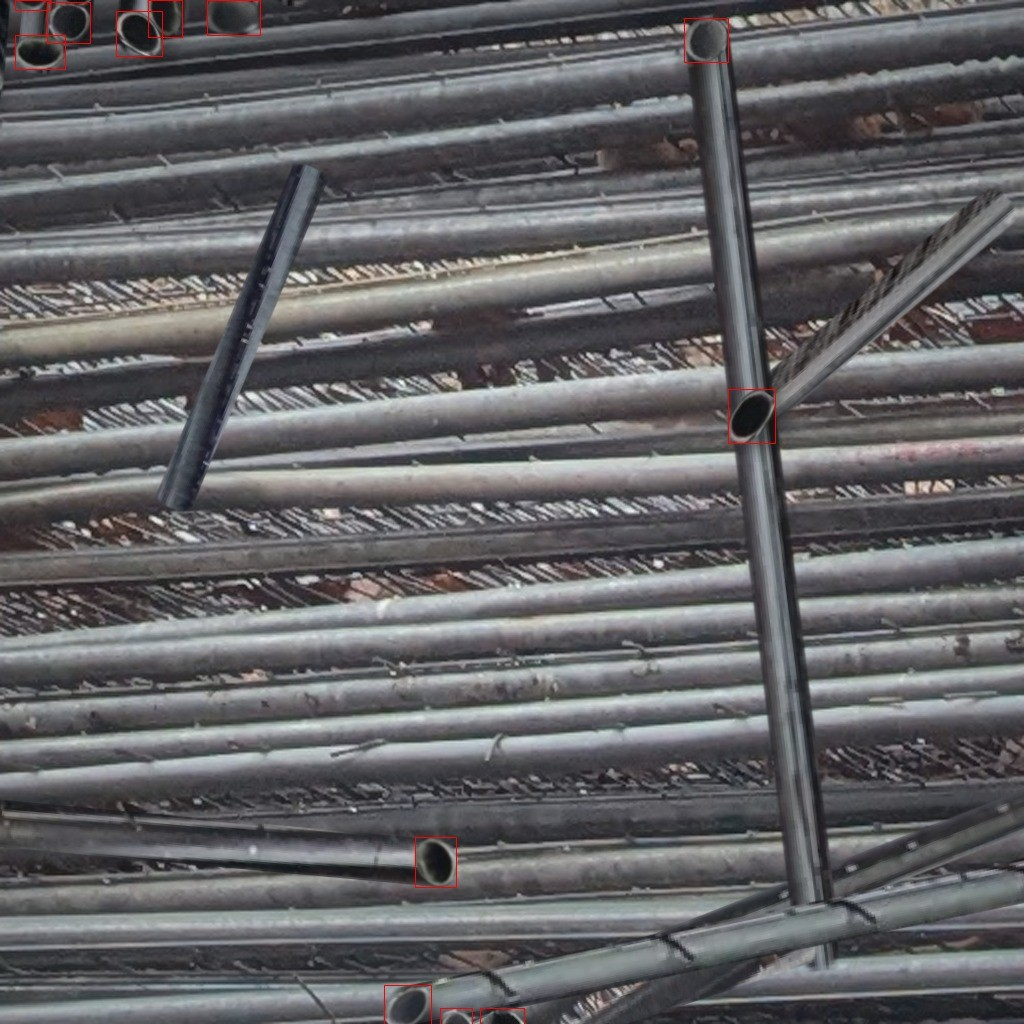
\includegraphics[width=\textwidth]{abbildungen/synth_003.jpg}
\end{subfigure}\hfill
\begin{subfigure}{0.245\textwidth}
  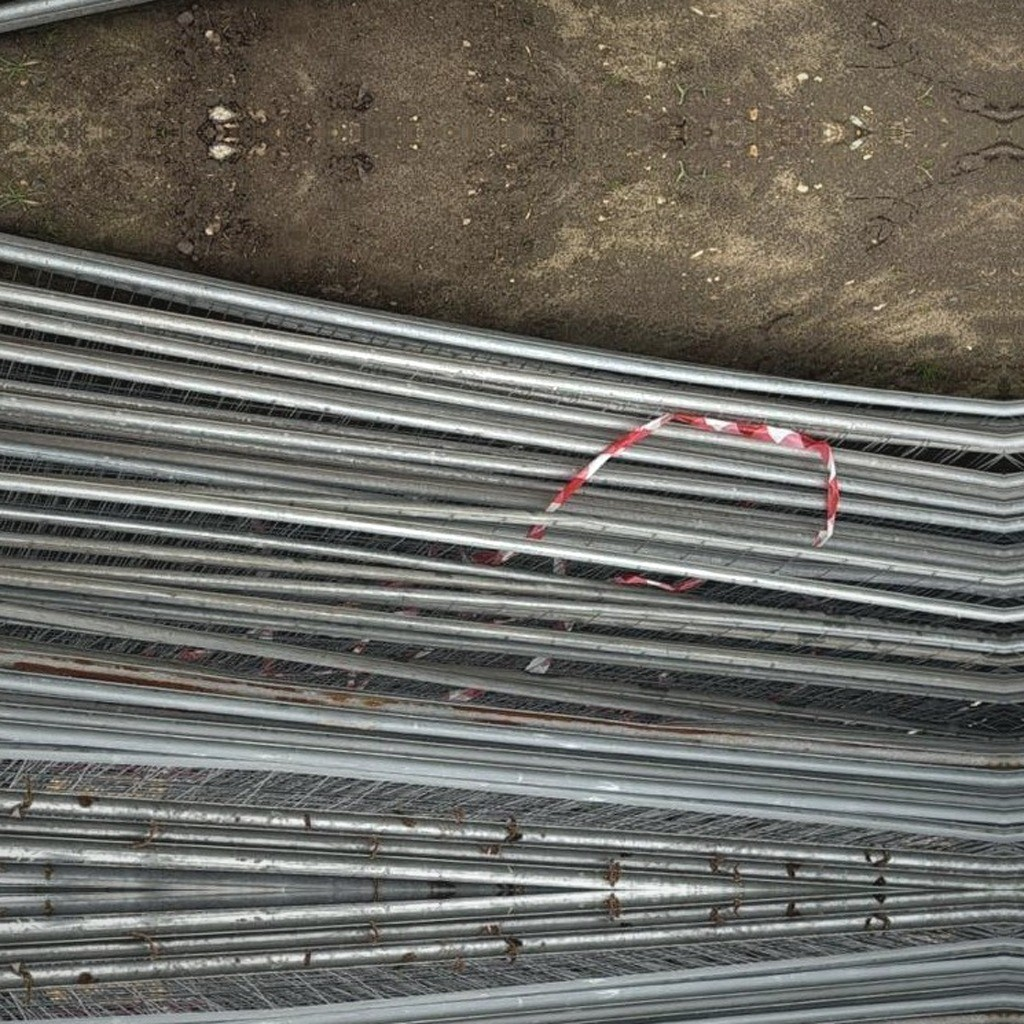
\includegraphics[width=\textwidth]{abbildungen/synth_004.jpg}
\end{subfigure}
\caption[Beispiele synthetischer Trainingsbilder]{Vier synthetische
Trainingsbilder mit den erzeugten Labels. Erkennbar sind die Clusterstruktur des
Layoutmodells, die Rohrschäfte hinter den Stirnflächen, die quer liegenden
Okkluder und die abgedunkelten Mulden.}
\label{abb:synthbeispiele}
\end{figure}

\begin{figure}[htbp]
\centering
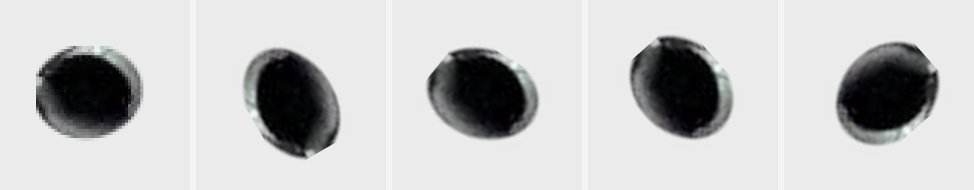
\includegraphics[width=\textwidth]{abbildungen/stufe_T2_geometrie.png}

\vspace{6pt}
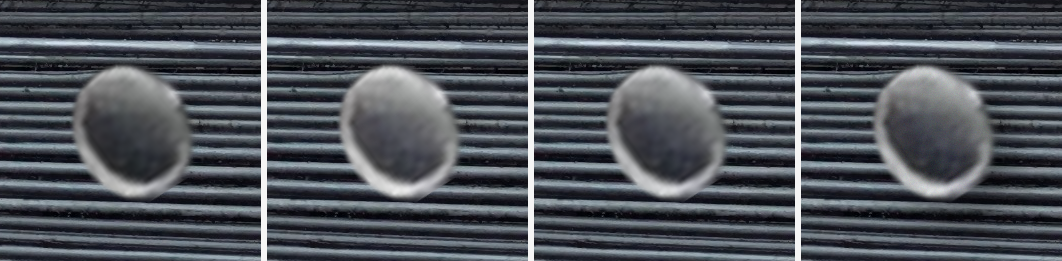
\includegraphics[width=\textwidth]{abbildungen/stufe_T3_photometrie.png}
\caption[Instanzgeometrie und Photometrie im Detail]{Die Stufen T2 und T3,
vergrößert. \emph{Oben (T2 Instanzgeometrie),
von links nach rechts:} der Quellausschnitt und vier Ziehungen aus $p(t)$ --
Rotation über den vollen Kreis, Skalierung, Ovalisierung, Delle, Perspektive.
Alle fünf Kacheln zeigen dasselbe Objekt bei gleichem Durchmesser.
\emph{Unten (T3 Photometrie), von links nach rechts:} dieselbe Instanz auf
demselben Hintergrund -- roh eingefügt, dann mit Photometrie, dann mit
Farbangleich, dann mit Einbettung und Schlagschatten. Der Farbangleich nach
Gleichung~\eqref{eq:harmonize} verschiebt die Verteilung nur teilweise; die
Einbettung ergänzt Kantenweichzeichnung, Rauschangleich nach
Gleichung~\eqref{eq:noise} und Schlagschatten. Für die Darstellung ist der
Zieldurchmesser auf 100\px{} gesetzt; im Datensatz liegt er bei 12--44\px.
Erzeugt mit \code{paper/tools/fig\_stufen.py}.}
\label{abb:stufendetail}
\end{figure}

\begin{figure}[htbp]
\centering
\begin{subfigure}{0.62\textwidth}
  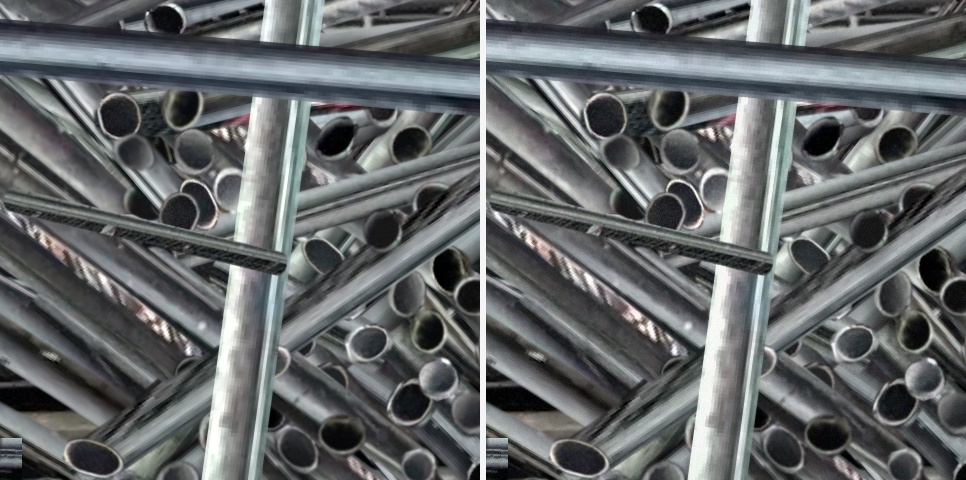
\includegraphics[width=\textwidth]{abbildungen/stufe_T8_global.jpg}
  \caption{T8 globale Bildstufe}
\end{subfigure}\hfill
\begin{subfigure}{0.35\textwidth}
  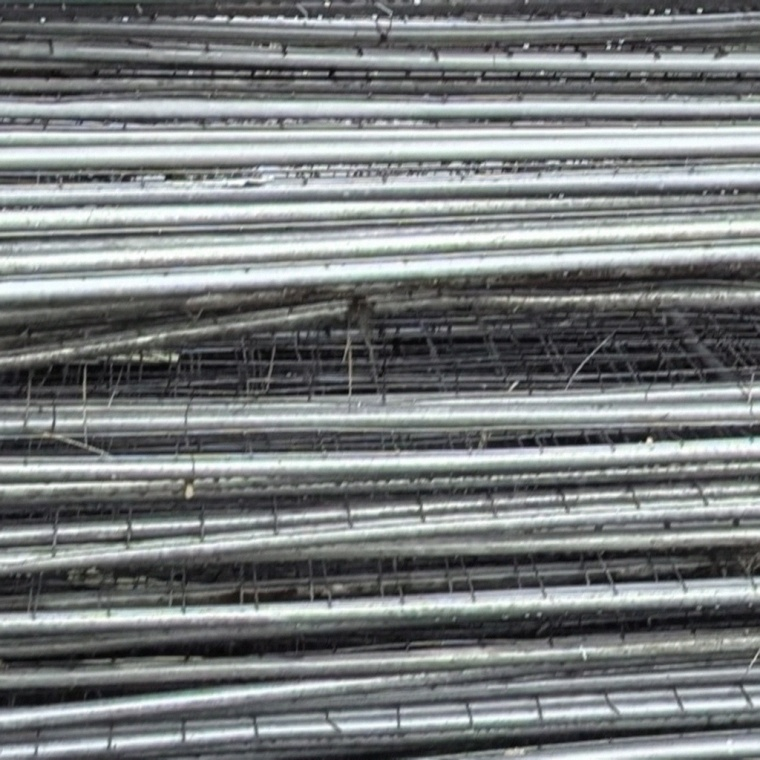
\includegraphics[width=\textwidth]{abbildungen/stufe_T9_negativ.jpg}
  \caption{T9 Negativbild}
\end{subfigure}
\caption[Globale Bildstufe und Negativbild]{Die Stufen T8 und T9.
(a)~Derselbe Bildausschnitt links ohne, rechts mit der globalen Stufe:
Helligkeit und
Kontrast, HSV, Defokus, Bewegungsunschärfe, Rauschen, Vignettierung und
JPEG-Requantisierung wirken auf das \emph{fertige} Bild und damit auf
eingefügte und originale Pixel gleichermaßen -- das ist ihr Zweck, denn ein
Unterschied in genau diesen Größen wäre eine Abkürzung im Sinne von
Tabelle~\ref{tab:signaturen}. (b)~Ein Negativbild: 9,7\,\% der Bilder enthalten
kein einziges Objekt. Gezeigt ist der schwierige Fall -- ein Rohrstapel
\emph{ohne} sichtbare Stirnflächen, also genau der Kontext, in dem Fehlalarme
entstehen. Erzeugt mit \code{paper/tools/fig\_stufen.py}.}
\label{abb:stufenglobal}
\end{figure}

\begin{figure}[htbp]
\centering
\begin{subfigure}{\textwidth}
  \centering
  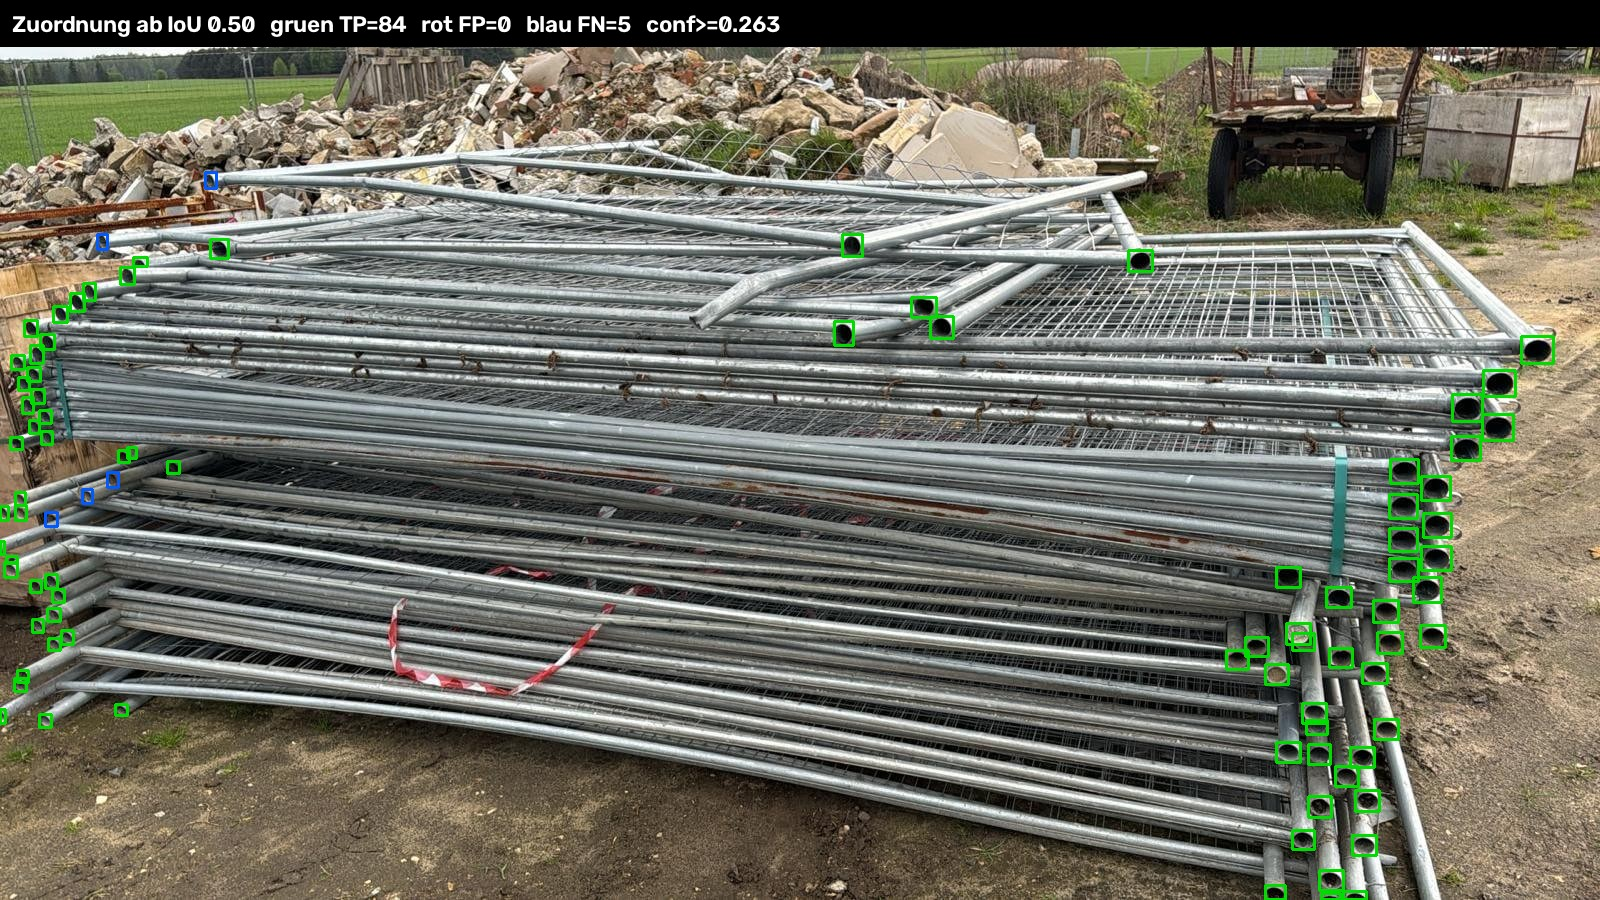
\includegraphics[width=0.93\textwidth]{abbildungen/qual_test_iou050.jpg}
  \caption{Zuordnung ab IoU 0,50 -- die berichtete Konvention.}
  \label{abb:qualitativ050}
\end{subfigure}

\vspace{3mm}
\begin{subfigure}{\textwidth}
  \centering
  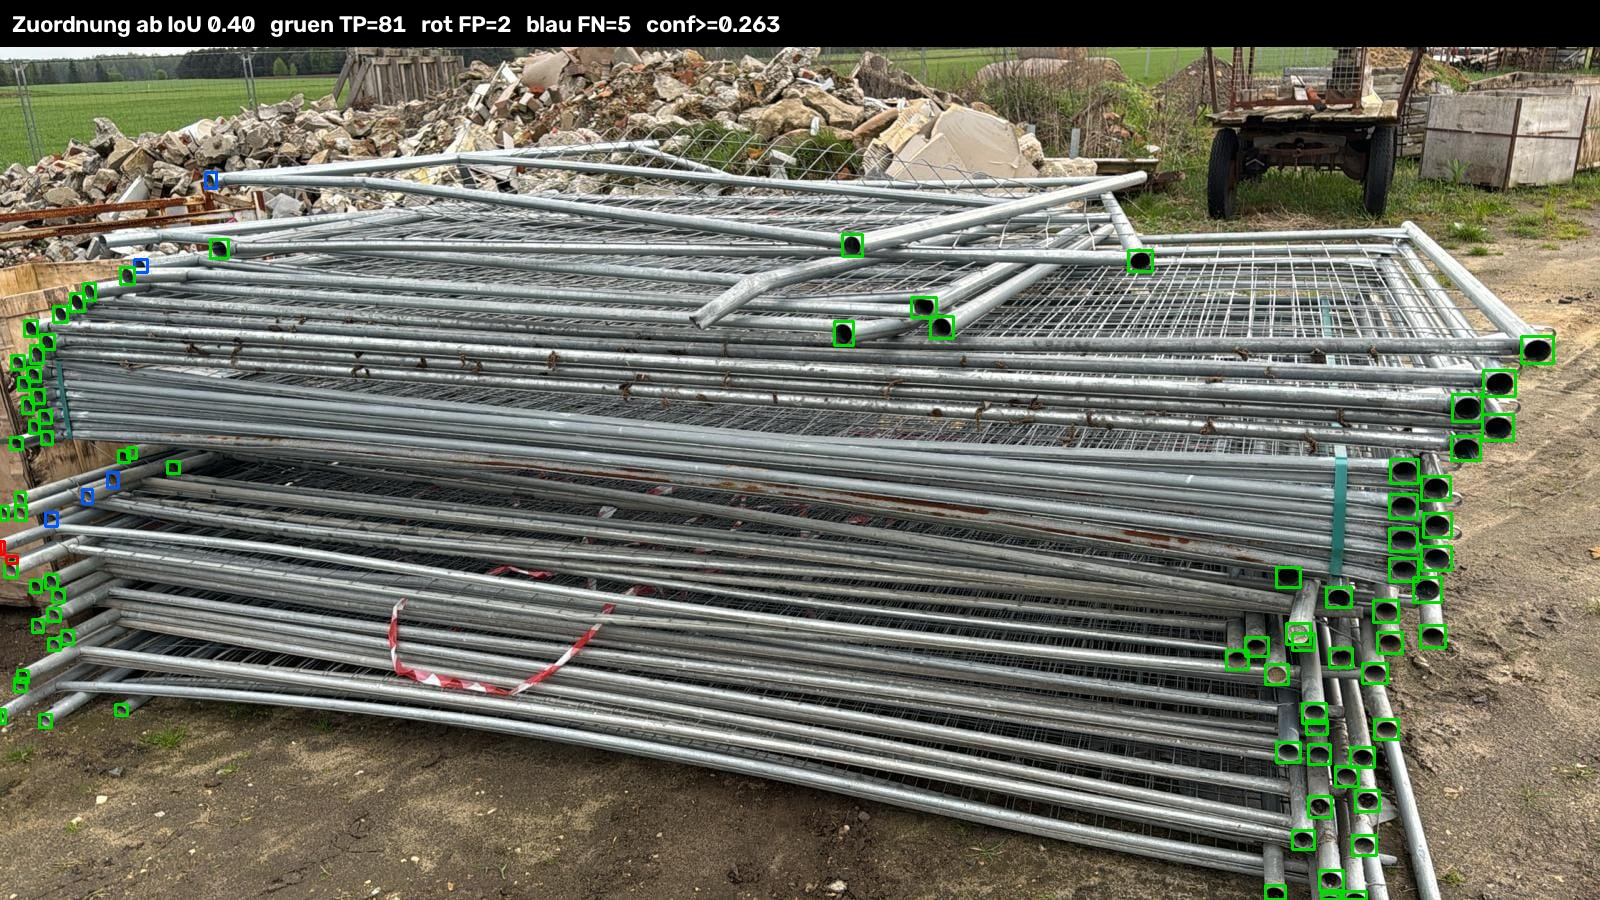
\includegraphics[width=0.93\textwidth]{abbildungen/qual_test_iou040.jpg}
  \caption{Zuordnung ab IoU 0,40 -- nur zur Diagnose.}
  \label{abb:qualitativ040}
\end{subfigure}
\caption[Qualitatives Ergebnis bei zwei Zuordnungsschwellen]{Qualitatives
Ergebnis auf \code{test}. Grün = Treffer, rot = Falsch-Positiv, blau =
Falsch-Negativ. \textbf{Beide Bilder zeigen dieselben 83 Detektionen} bei
derselben Konfidenzschwelle; verändert wurde ausschließlich die IoU-Schwelle der
Zuordnung. Von 0,50 auf 0,40 verschwinden sechs der acht Falsch-Positiven
\emph{und} sechs der elf Falsch-Negativen -- es sind dieselben sechs Objekte,
die bei 0,50 doppelt als Fehler gezählt werden
(Abschnitt~\ref{sec:boxversatz}). Die untere Darstellung belegt damit, dass es
sich um Zuordnungsartefakte handelt; sie ist \emph{kein} Ersatz für die
berichteten Metriken, denn 0,50 ist die Konvention von PASCAL VOC und COCO
\parencite{everingham2010,lin2014coco}. Behoben wird die Ursache nicht durch
eine andere Schwelle, sondern durch die Angleichung der Labelkonvention.}
\label{abb:qualitativ}
\end{figure}



\end{document}
